\documentclass[journal]{vgtc}                % final (journal style)
%\documentclass[review,journal]{vgtc}         % review (journal style)
%\documentclass[widereview]{vgtc}             % wide-spaced review
%\documentclass[preprint,journal]{vgtc}       % preprint (journal style)
%\documentclass[electronic,journal]{vgtc}     % electronic version, journal

%% Uncomment one of the lines above depending on where your paper is
%% in the conference process. ``review'' and ``widereview'' are for review
%% submission, ``preprint'' is for pre-publication, and the final version
%% doesn't use a specific qualifier. Further, ``electronic'' includes
%% hyperreferences for more convenient online viewing.

%% Please use one of the ``review'' options in combination with the
%% assigned online id (see below) ONLY if your paper uses a double blind
%% review process. Some conferences, like IEEE Vis and InfoVis, have NOT
%% in the past.

%% Please note that the use of figures other than the optional teaser is not permitted on the first page
%% of the journal version.  Figures should begin on the second page and be
%% in CMYK or Grey scale format, otherwise, colour shifting may occur
%% during the printing process.  Papers submitted with figures other than the optional teaser on the
%% first page will be refused.

%% These three lines bring in essential packages: ``mathptmx'' for Type 1
%% typefaces, ``graphicx'' for inclusion of EPS figures. and ``times''
%% for proper handling of the times font family.

\usepackage{mathptmx}
\usepackage{graphicx}
\usepackage{times}
\usepackage{subcaption}
\usepackage{amsmath}

%MC Stuff
\newcommand{\todo}[1]{\textbf{\textcolor{red}{TODO: #1}}\\}

%% We encourage the use of mathptmx for consistent usage of times font
%% throughout the proceedings. However, if you encounter conflicts
%% with other math-related packages, you may want to disable it.

%% This turns references into clickable hyperlinks.
\usepackage[bookmarks,backref=true,linkcolor=black]{hyperref} %,colorlinks
\hypersetup{
  pdfauthor = {},
  pdftitle = {},
  pdfsubject = {},
  pdfkeywords = {},
  colorlinks=true,
  linkcolor= black,
  citecolor= black,
  pageanchor=true,
  urlcolor = black,
  plainpages = false,
  linktocpage
}

%% If you are submitting a paper to a conference for review with a double
%% blind reviewing process, please replace the value ``0'' below with your
%% OnlineID. Otherwise, you may safely leave it at ``0''.
\onlineid{0}

%% declare the category of your paper, only shown in review mode
\vgtccategory{Research}

%% allow for this line if you want the electronic option to work properly
\vgtcinsertpkg

%% In preprint mode you may define your own headline.
%\preprinttext{To appear in an IEEE VGTC sponsored conference.}

%% Paper title.

\title{Surprise! Bayesian Weighting for De-Biasing Thematic Maps}

%% This is how authors are specified in the journal style

%% indicate IEEE Member or Student Member in form indicated below
\author{Michael Correll and Jeffrey Heer}
\authorfooter{
%% insert punctuation at end of each item
\item
 Michael Correll is with the University of Washington. E-mail: correll@uw.edu.
\item
 Jeffrey Heer is with the University of Washington. E-mail: jheer@uw.edu.
}

%other entries to be set up for journal
\shortauthortitle{Correll and Heer: Surpise! Bayesian Weighting of Thematic Maps}
%\shortauthortitle{Firstauthor \MakeLowercase{\textit{et al.}}: Paper Title}

%% Abstract section.
\abstract{Thematic maps are commonly used for visualizing the density of events in spatial data. However, these maps can mislead by giving visual prominence to known base rates (such as population densities) or to artifacts of sample size and normalization (such as outliers arising from smaller, and thus more variable, samples). In this work, we adapt Bayesian surprise to generate maps that counter these biases. Bayesian surprise, which has shown promise for modeling human visual attention, weights information with respect to how it updates beliefs over a space of models. We introduce Surprise Maps, a visualization technique that weights event data relative to a set of spatio-temporal models. Unexpected events (those that induce large changes in belief over the model space) are visualized more prominently than those that follow expected patterns. Using both synthetic and real-world datasets, we demonstrate how Surprise Maps overcome some limitations of traditional event maps.
} % end of abstract

%% Keywords that describe your work. Will show as 'Index Terms' in journal
%% please capitalize first letter and insert punctuation after last keyword
\keywords{Thematic Maps, Bayesian Surprise, Event Visualization, Spatio-temporal data}

%% ACM Computing Classification System (CCS).
%% See <http://www.acm.org/class/1998/> for details.
%% The ``\CCScat'' command takes four arguments.

%\CCScatlist{ % not used in journal version
% \CCScat{K.6.1}{Management of Computing and Information Systems}%
%{Project and People Management}{Life Cycle};
% \CCScat{K.7.m}{The Computing Profession}{Miscellaneous}{Ethics}
%}

\newcommand{\teaserFig}{
  \teaser{
		\centering
		\begin{subfigure}[t]{.3\textwidth}
			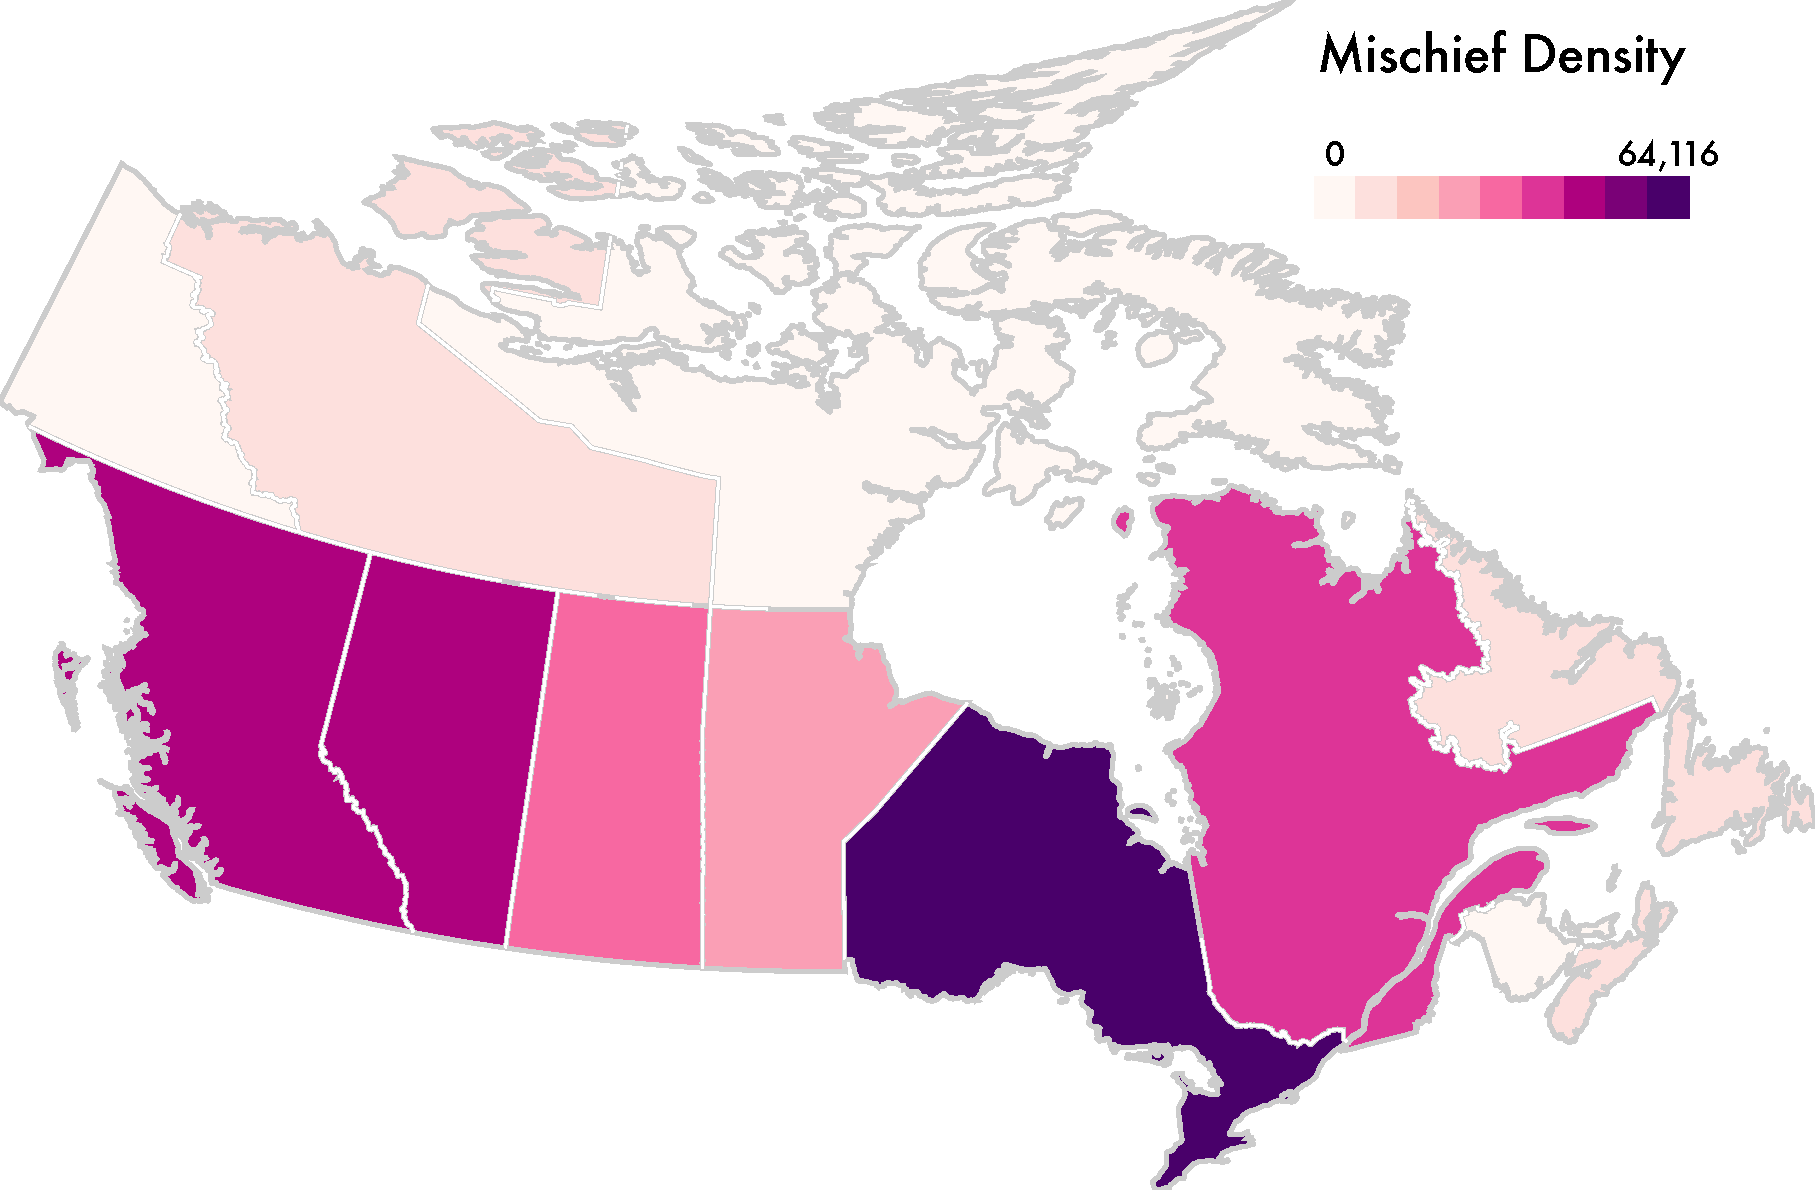
\includegraphics[width=\textwidth]{figures/canada-density}
			\caption{The \textbf{Event Density} of ``mischief'' in Canada.}
			\label{fig:canadadensity}
		\end{subfigure}
		~
		\begin{subfigure}[t]{.3\textwidth}
			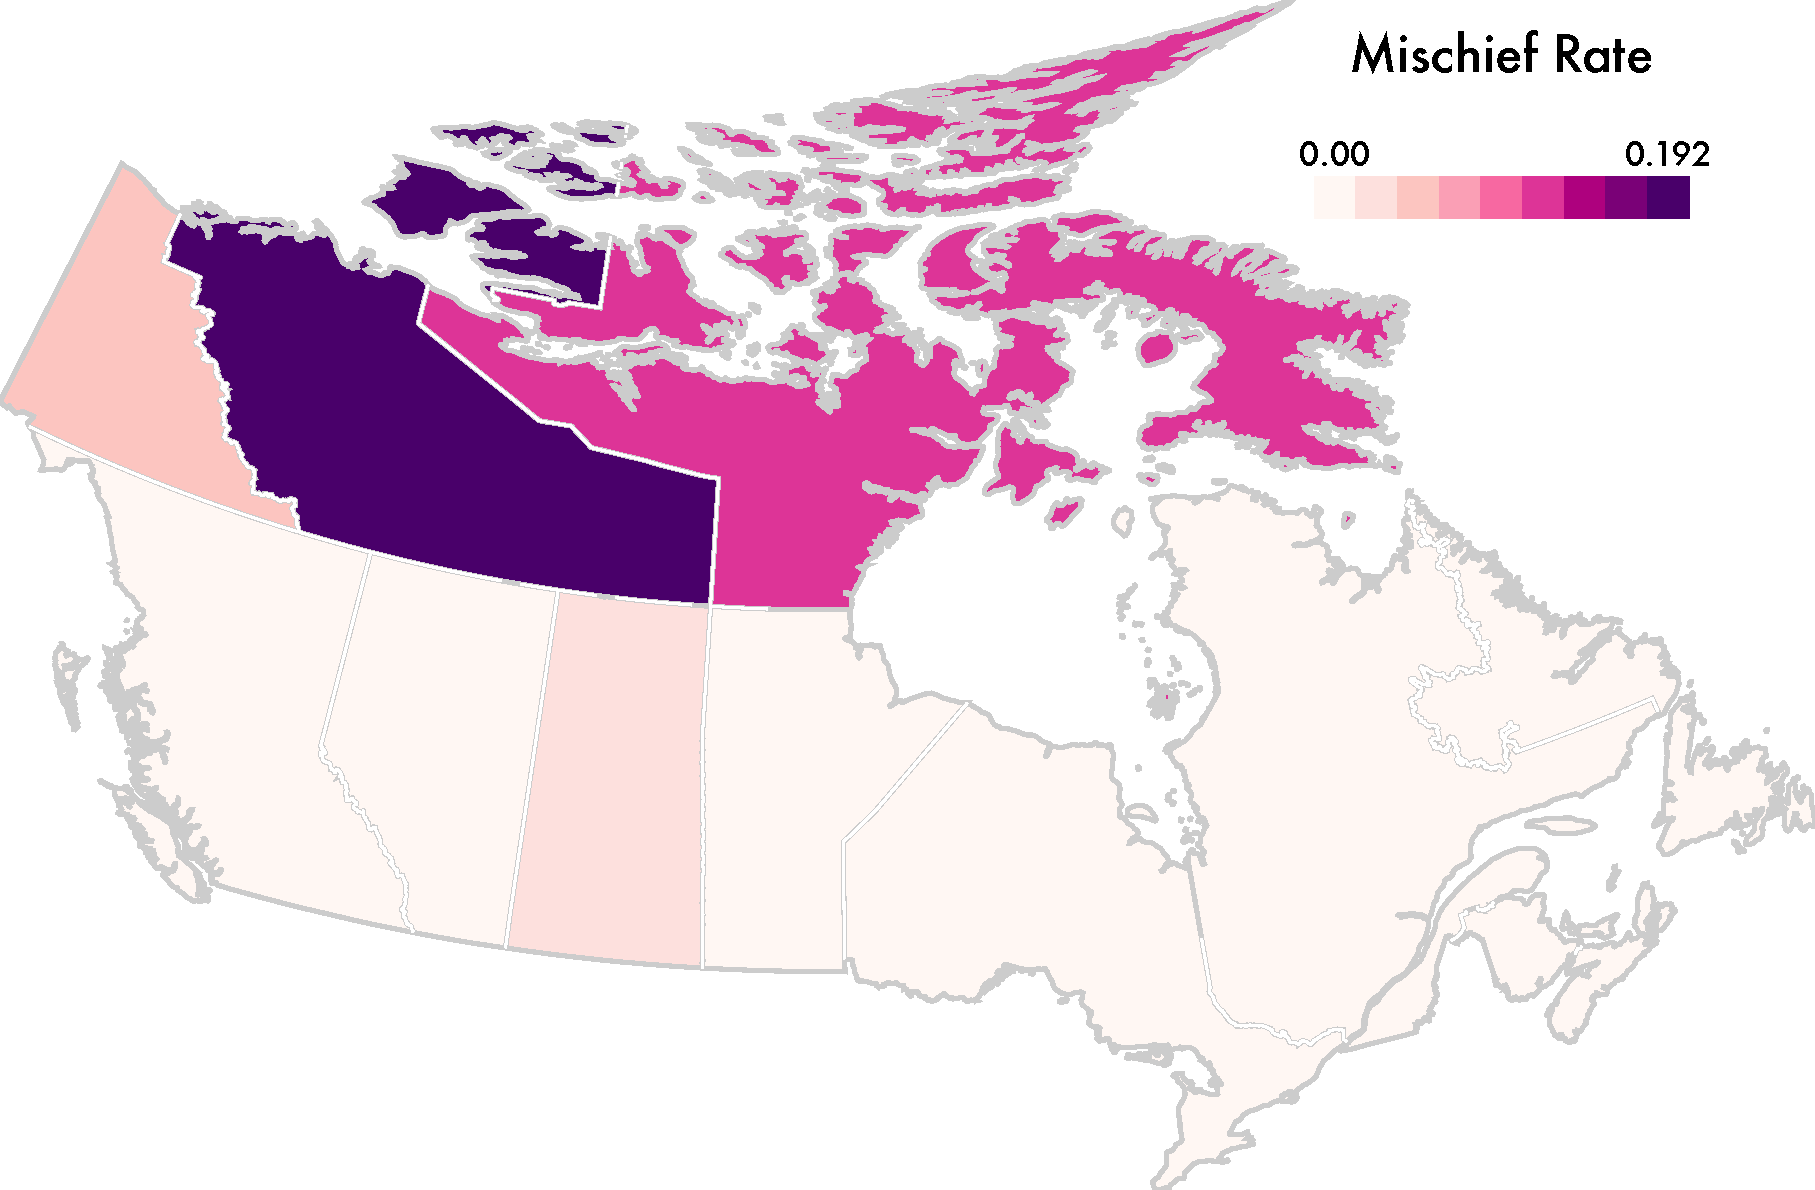
\includegraphics[width=\textwidth]{figures/canada-rate}
			\caption{The per-capita \textbf{Event Rate} of mischief.}
			\label{fig:canadarate}
		\end{subfigure}
		~
		\begin{subfigure}[t]{.3\textwidth}
			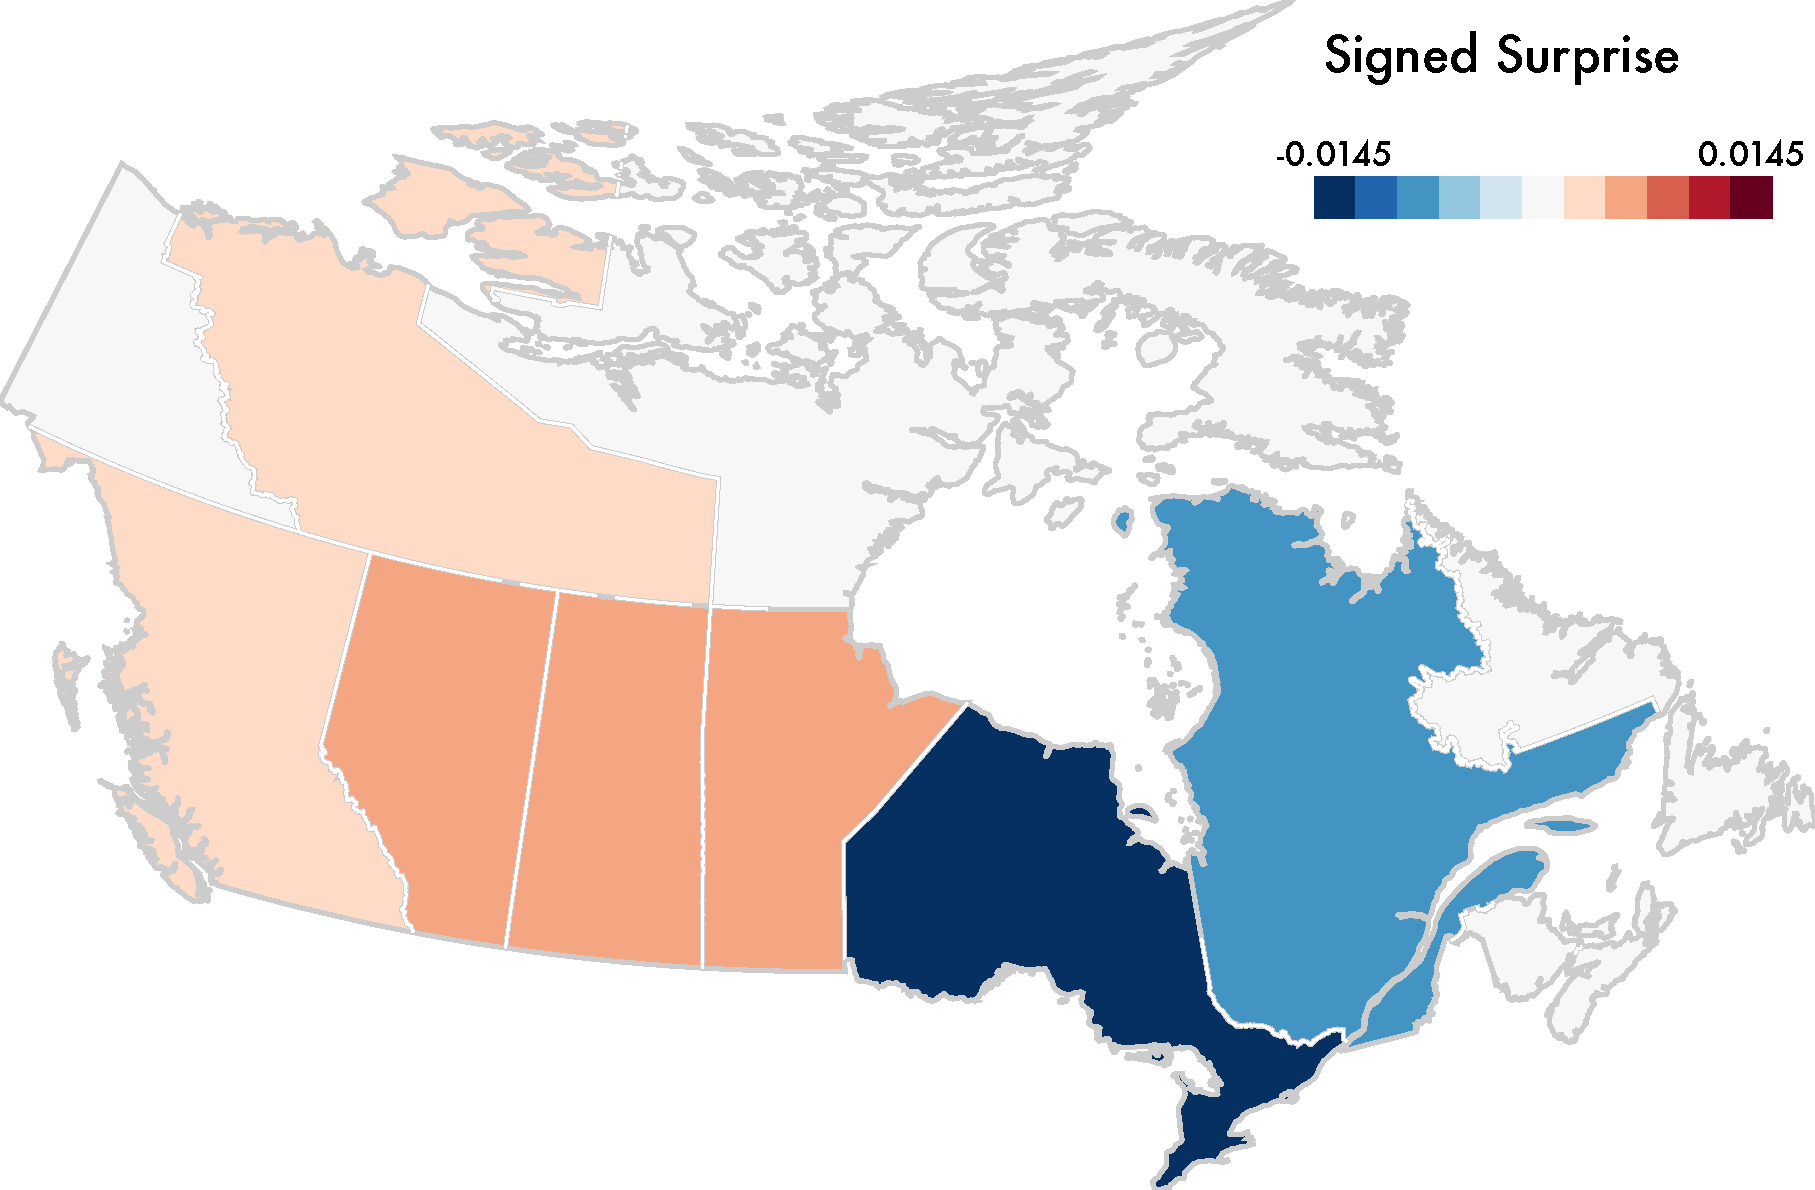
\includegraphics[width=\textwidth]{figures/canada-surprise2}
			\caption{The \textbf{Surprise Map} of mischief. }
			\label{fig:canadasurprise}
		\end{subfigure}
		\caption{ Choropleth maps of (a) event density, (b) per-capita event rates, and (c) Bayesian surprise for ``mischief'' (a class of property crime) in Canada. Which province or territory is safest? The density of crimes (Fig. \ref{fig:canadadensity}) in the southern provinces suggest that they are less safe; however, this is due to the much larger populations in those provinces. Normalizing to a per-capita rate (Fig. \ref{fig:canadarate}) gives the opposite impression. A Surprise Map (Fig. \ref{fig:canadasurprise}), using both population density and a de Moivre funnel as models, finds the provinces that stick out: Ontario and Quebec have crime rates lower than expected given their population. The seemingly high per-capita rates in Nunavut accord with the higher variability that can arise from a smaller population. }
	\label{fig:canada}
  }

}

\newcommand{\gaussFig}{
 \begin{figure*}
 \centering
 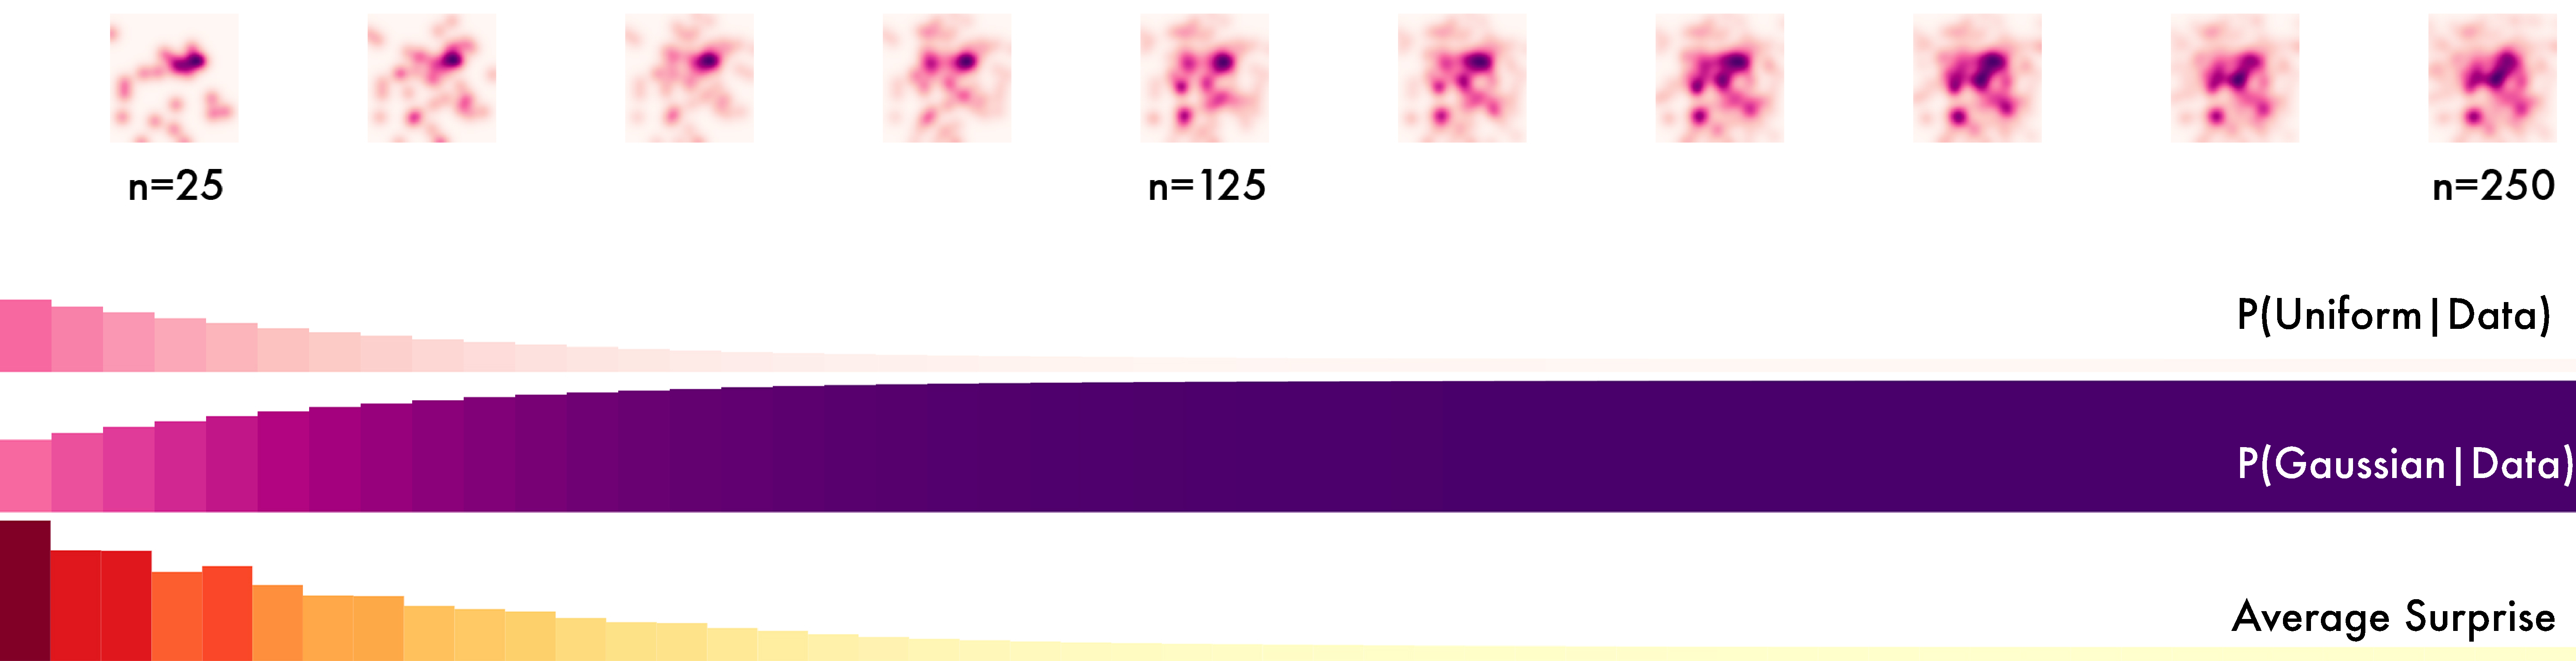
\includegraphics[width=.9\textwidth]{figures/gauss-2}
 \caption{
 	Changes in beliefs about spatial models leading to surprise. Here the events are sampled from a Gaussian distribution, and there are two proposed spatial models of events: a Gaussian (in this case, the correct model), and a uniform model. Initially, both models are equiprobable. However, as more events are processed, modes that are in keeping with a Gaussian model (but would be unlikely in a uniform model), adjust the modal beliefs in favor of the Gaussian model (causing surprise). Once the Gaussian model is established as the clear favorite, the surprise of events tapers off, asymptotically approaching 0. Probability histograms range from $[0,1]$, average surprise ranges from $[0,0.01]$ bits.
 }
 \label{fig:gauss}
 \end{figure*}
}

\newcommand{\funnelFig}{
	\begin{figure}
		\centering
		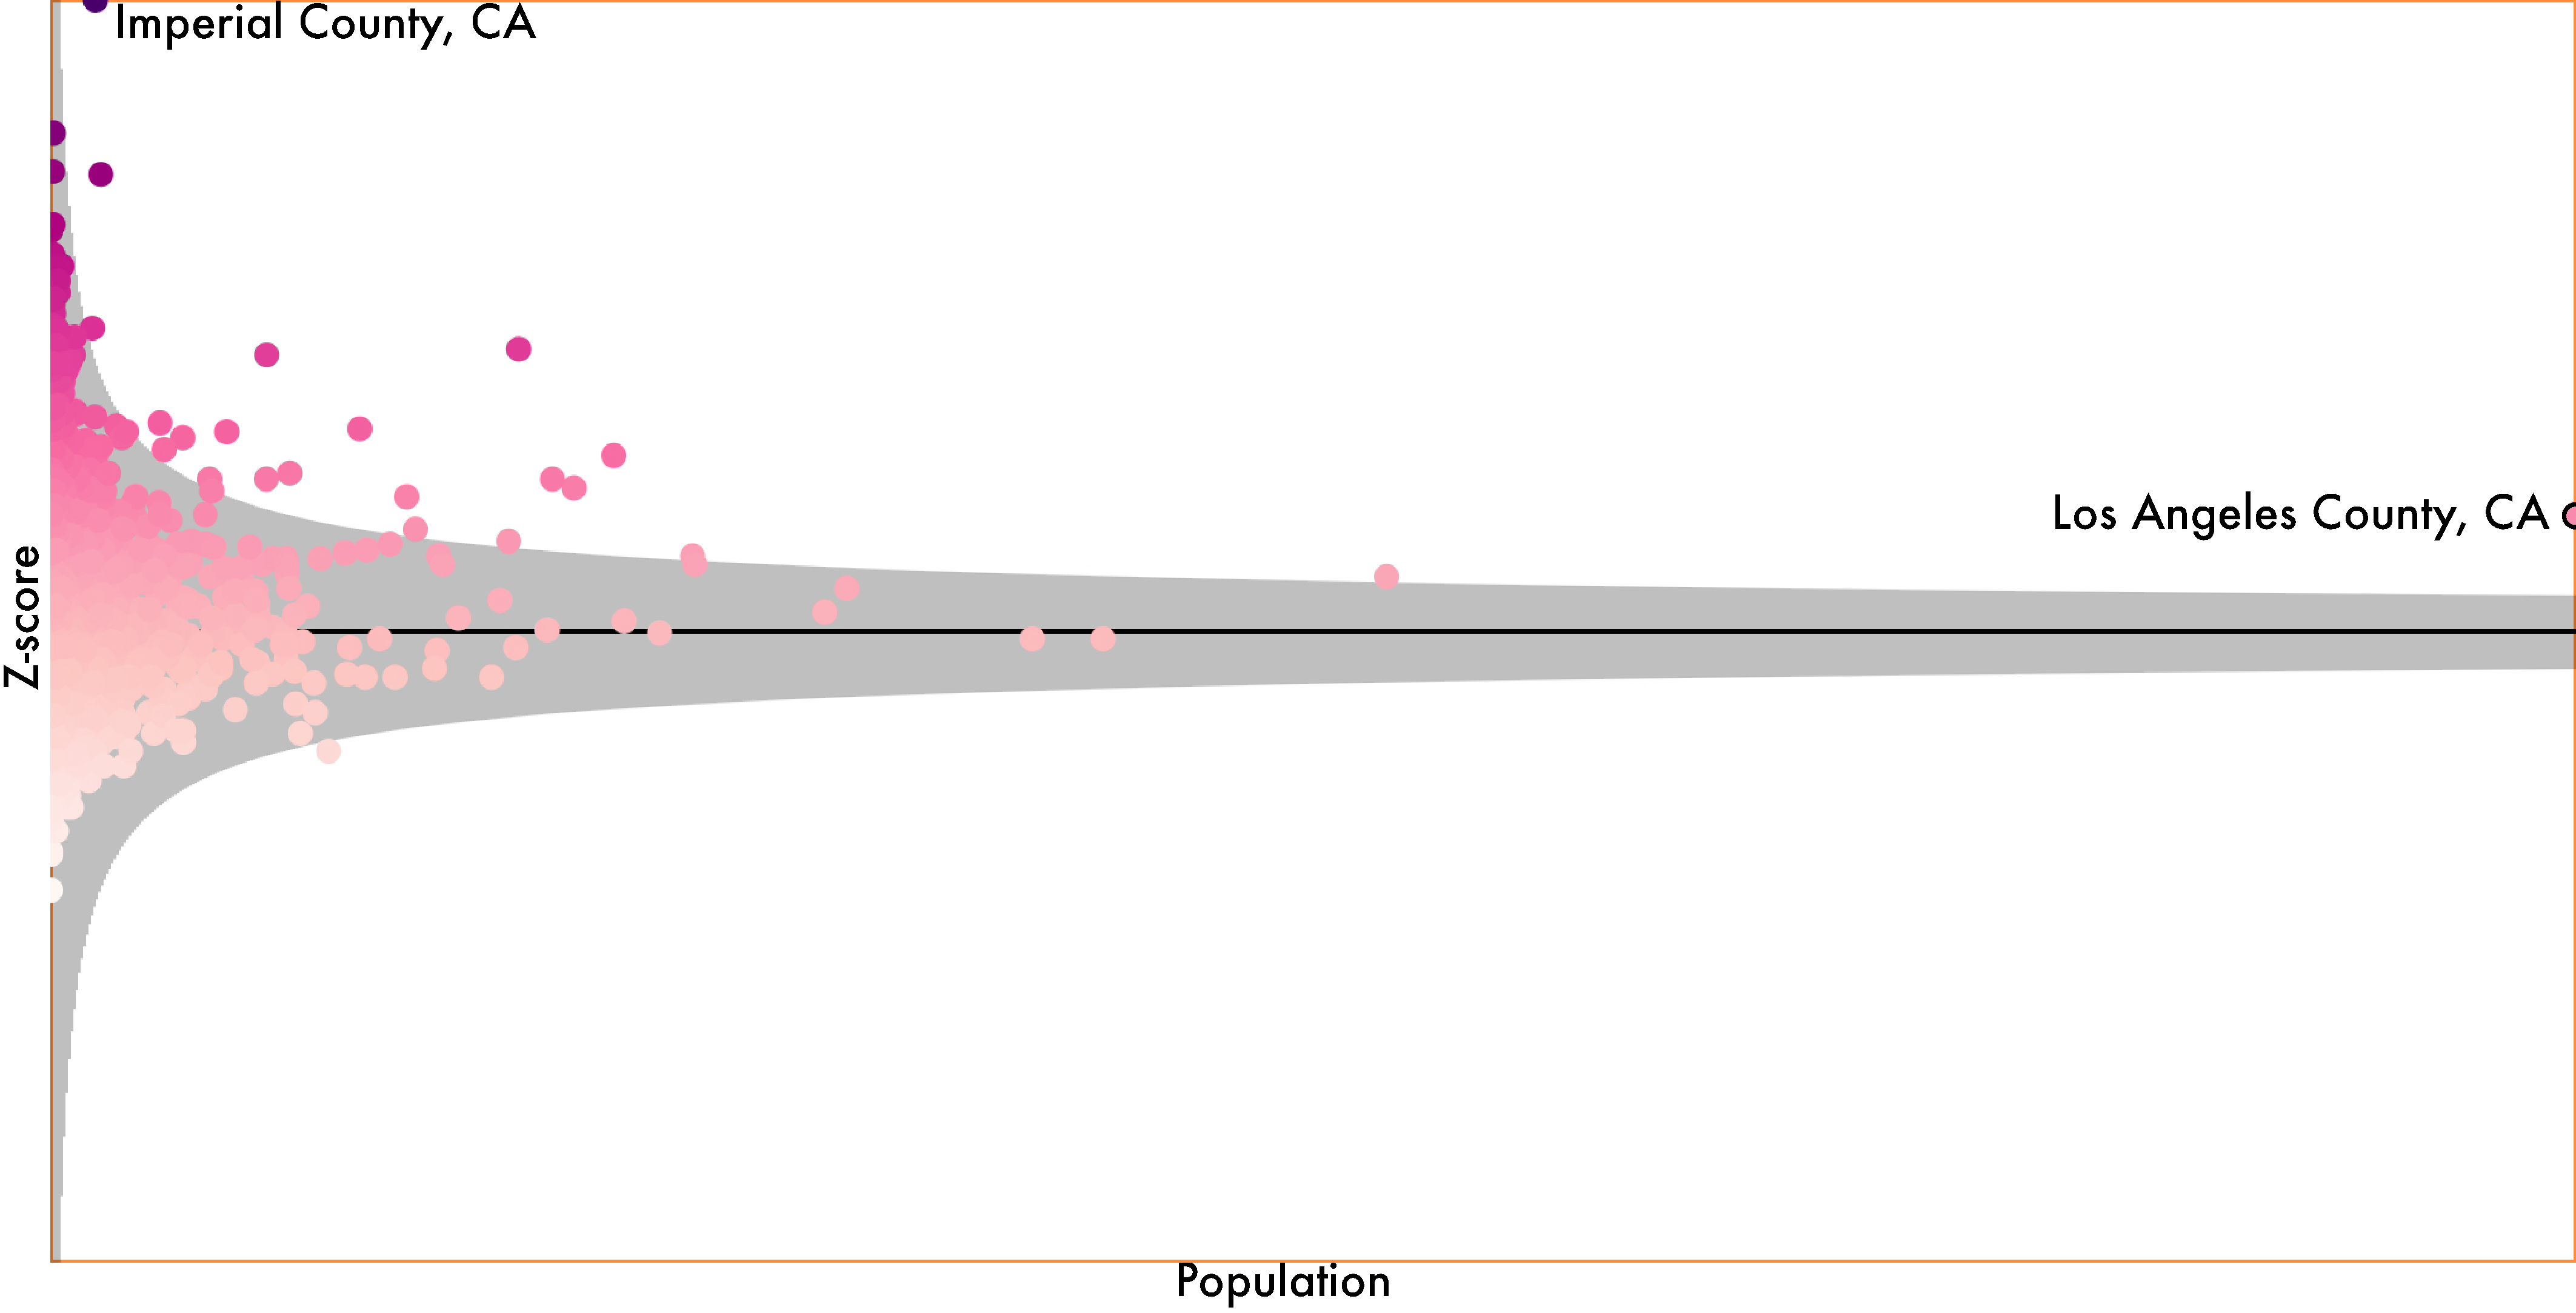
\includegraphics[width=.9\columnwidth]{figures/funnel}
		\caption{
			A funnel plot of the 2008 U.S. unemployment rate by county. The gray region depicts a 95\% confidence interval of the sample mean, using standard error. As sample size increases, variability decreases. Large differences in event rates may be an artifact of sample size. Conversely, small changes in event rate can be unexpected in high population regions. Some interesting counties (where $P(D|M)$ are low) are Imperial County, CA, which has a somewhat low population, but a high unemployment rate (30\%), and LA County, CA, which has an unemployment rate that is not much higher than the national average (12.7\%, versus an 8.7\% average), but is so populous that its higher rate is notable. Color encodes the unemployment rate, $[0,30\%]$.
		}
		\label{fig:funnel}
	\end{figure}
}


\newcommand{\gaussMaps}{
  \begin{figure}
  	\centering
    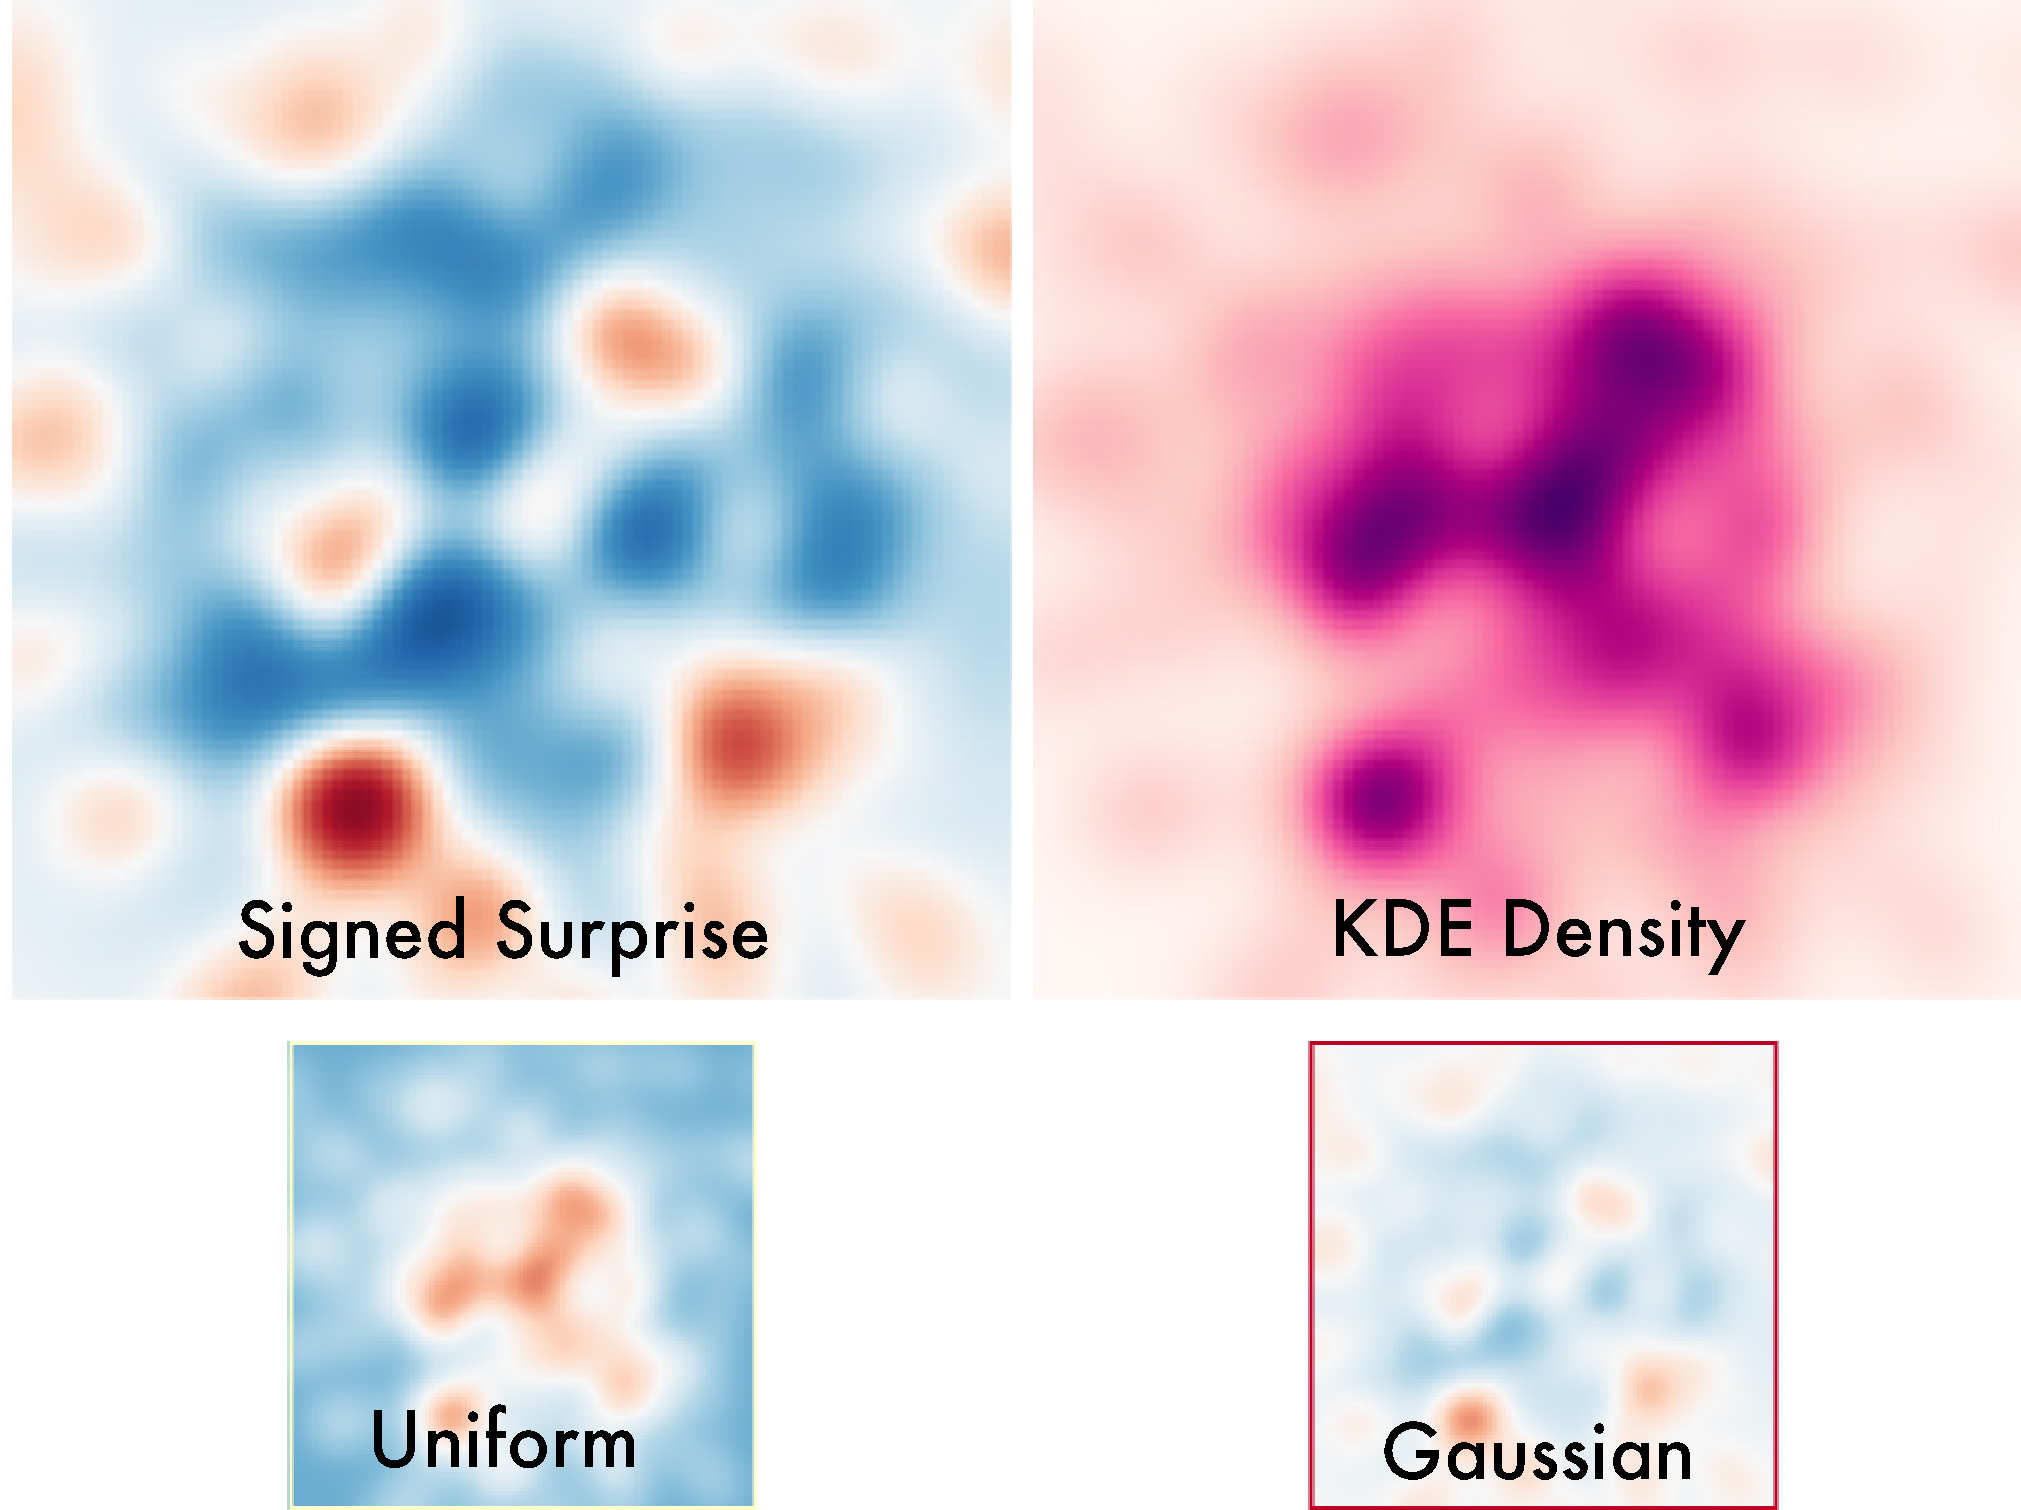
\includegraphics[width=.9\columnwidth]{figures/gauss2-2}
  	\caption{A Surprise Map from our synthetic dataset presented in \protect\S\ref{sec:synthetic}. The large heatmaps (top) show the signed surprise (left, from [-0.53,0.53]) and the KDE event density (right). The small heatmaps (bottom) show differences between observed data and the expectations provided by our spatial models. Blue regions are where we have seen fewer events than we expect, and red regions have more density than expected. After 250 events, belief in the Gaussian model is very close to 1. As such, the Surprise Map highlights deviations from the Gaussian model, in this case the red spatial outliers. Different model beliefs would produce a different weighting of events.
  	}
  	\label{fig:gaussMap}
  \end{figure}
}

\newcommand{\popFig}{
\begin{figure*}
	\centering
	\begin{subfigure}[tb]{0.3\textwidth}
		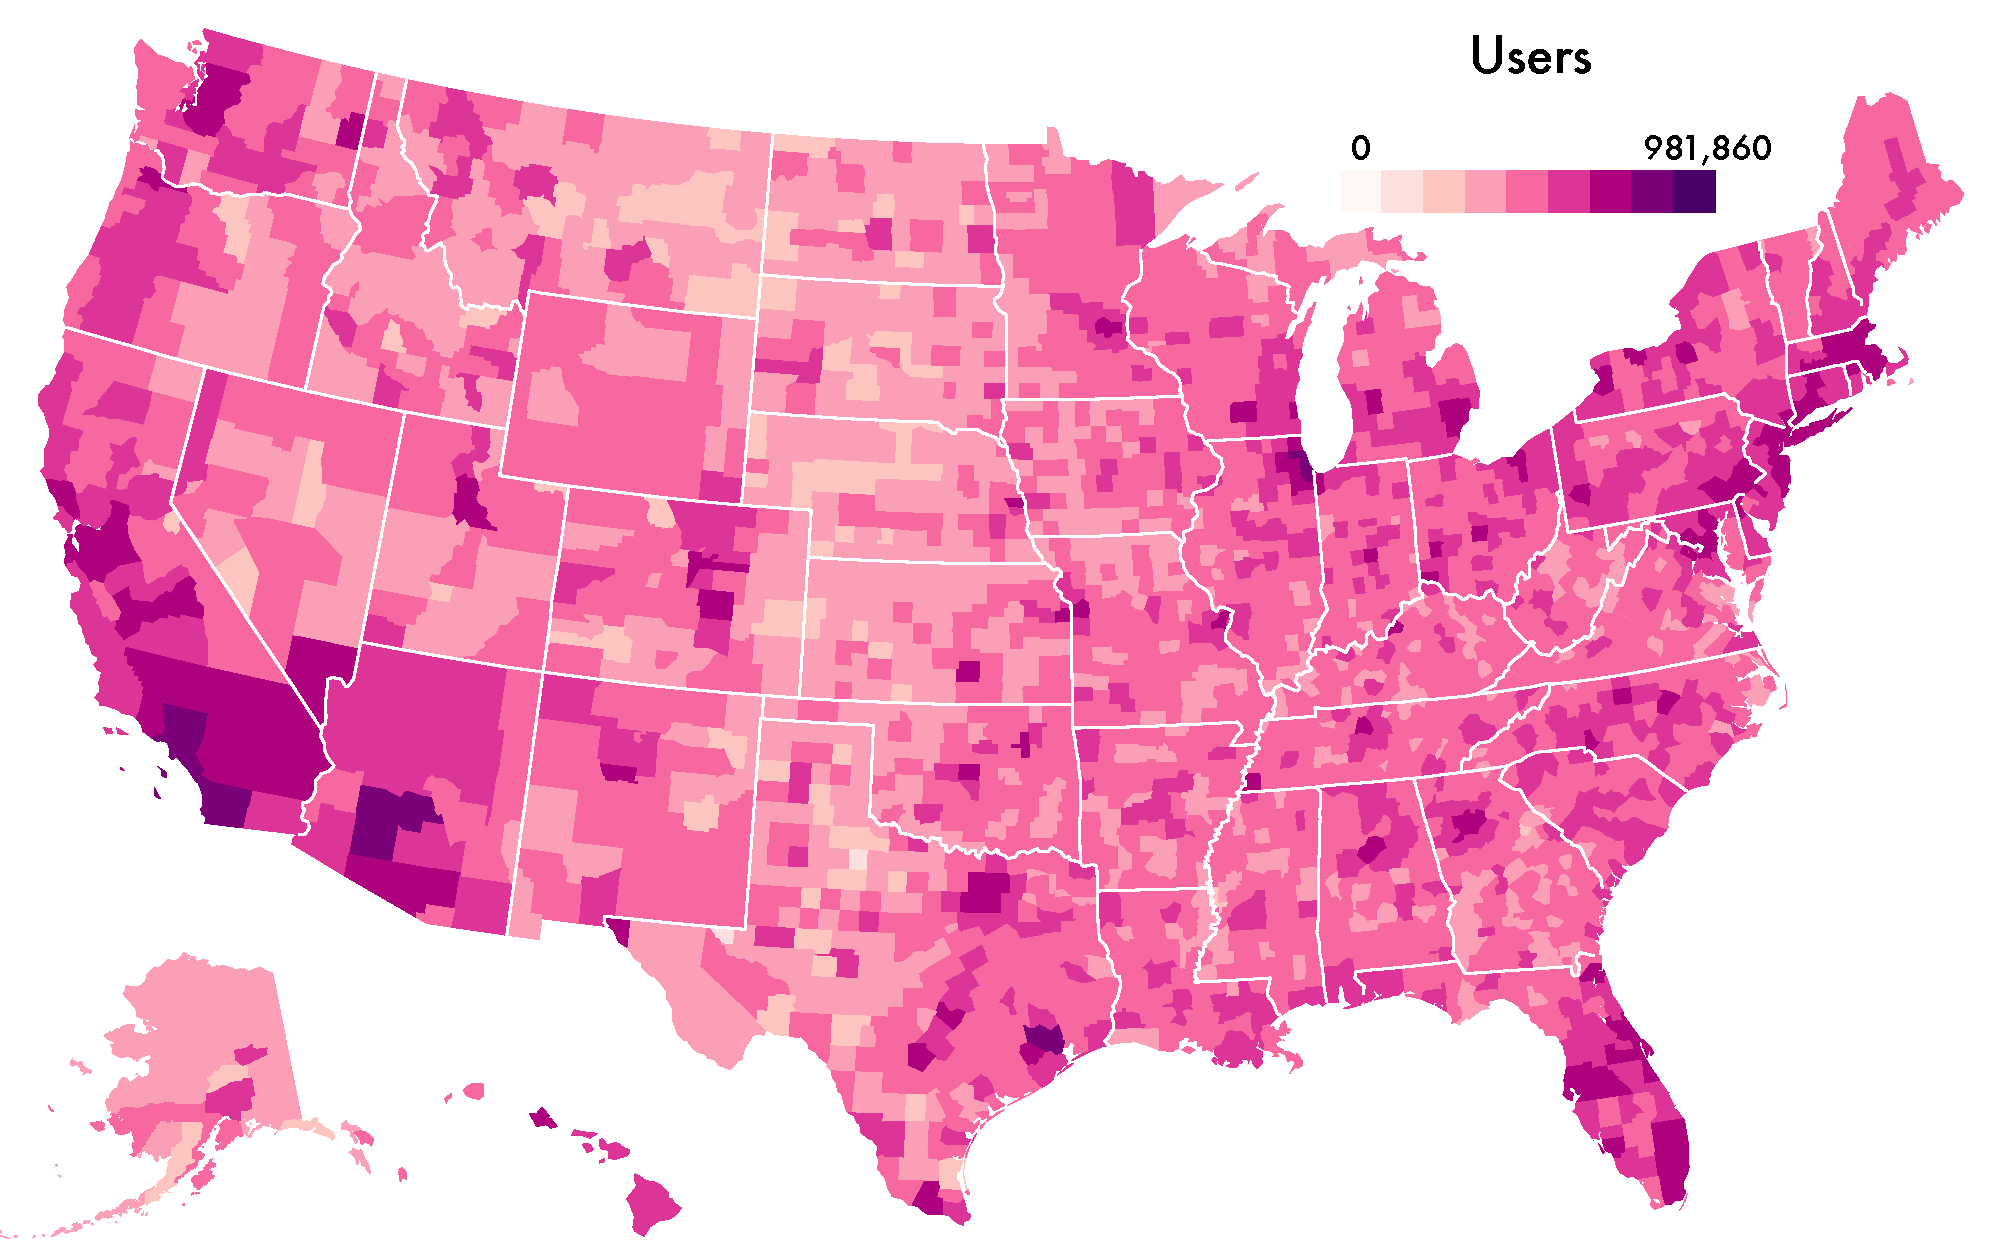
\includegraphics[width=\textwidth]{./figures/population1}
		\caption{Users of Application A}
		\label{fig:pop1}
	\end{subfigure}
	~
	\begin{subfigure}[tb]{0.3\textwidth}
		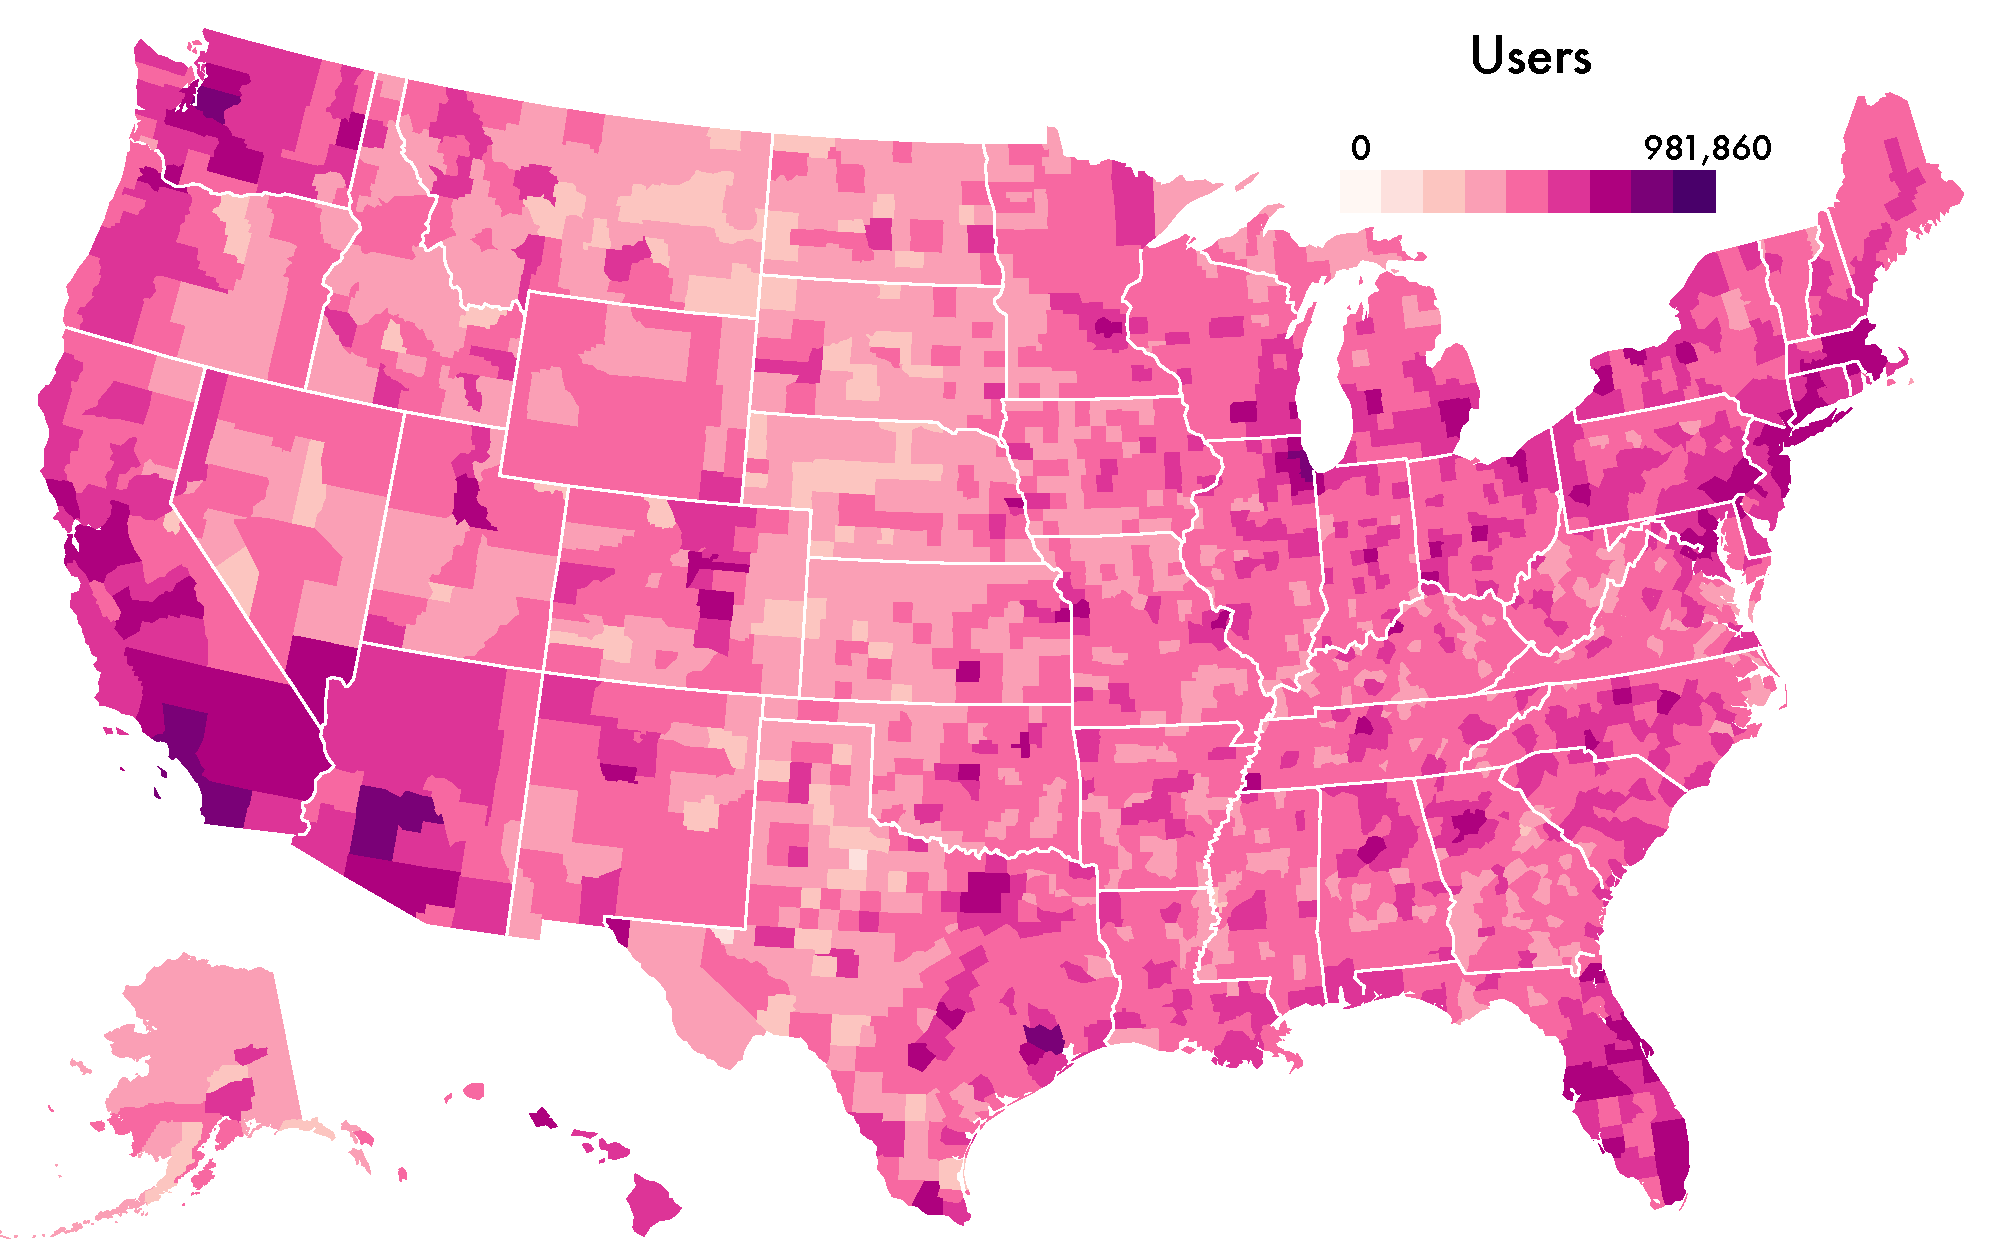
\includegraphics[width=\textwidth]{./figures/population2}
		\caption{Users of Application B}
		\label{fig:pop2}
	\end{subfigure}
	~
	\begin{subfigure}[tb]{0.3\textwidth}
		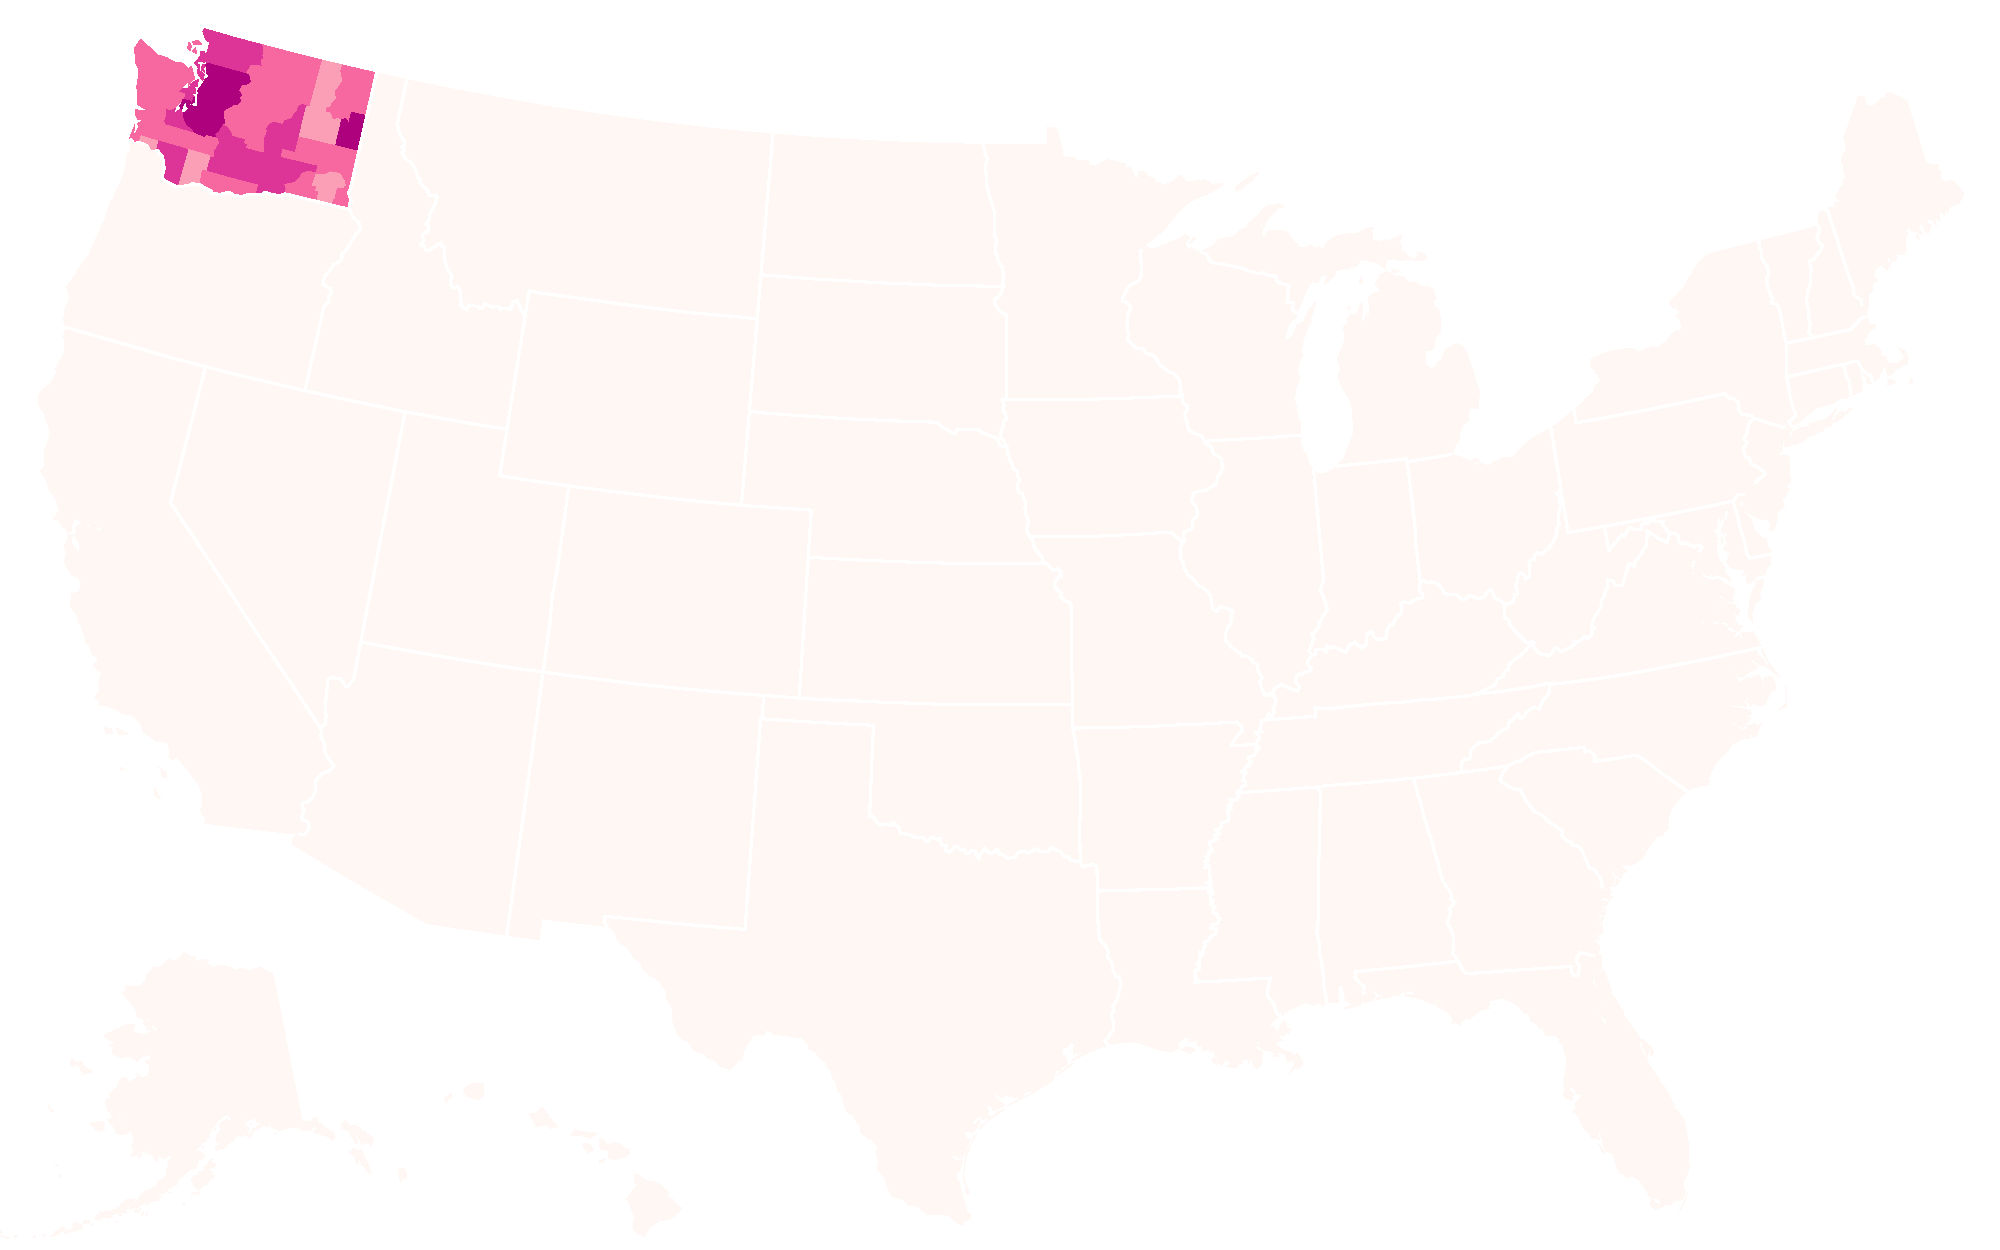
\includegraphics[width=\textwidth]{./figures/population}
		\caption{B-A}
		\label{fig:popdiff}
	\end{subfigure}
	\caption{Choropleth maps illustrating the base rate bias. By encoding only the unweighted density of events, the base rate or population rate of event occurrence is the dominant visual signal, making spatial comparisons difficult. These choropleth maps visualize the location of users of two fictional software applications, A and B. The usage patterns look very similar at a glance, but that is because usage largely follows population (a U.S. citizen is 10\% likely to use either application). An interesting spatial pattern\,---\,B has twice as many users in Washington state as A\,---\,is all but drowned out by the spatially complex, but largely task-irrelevant, signal of U.S. population density.}
	\label{fig:pop}
\end{figure*}
}

\newcommand{\poissonFig}{
\begin{figure*}
	\centering
	\begin{subfigure}[tb]{0.3\textwidth}
		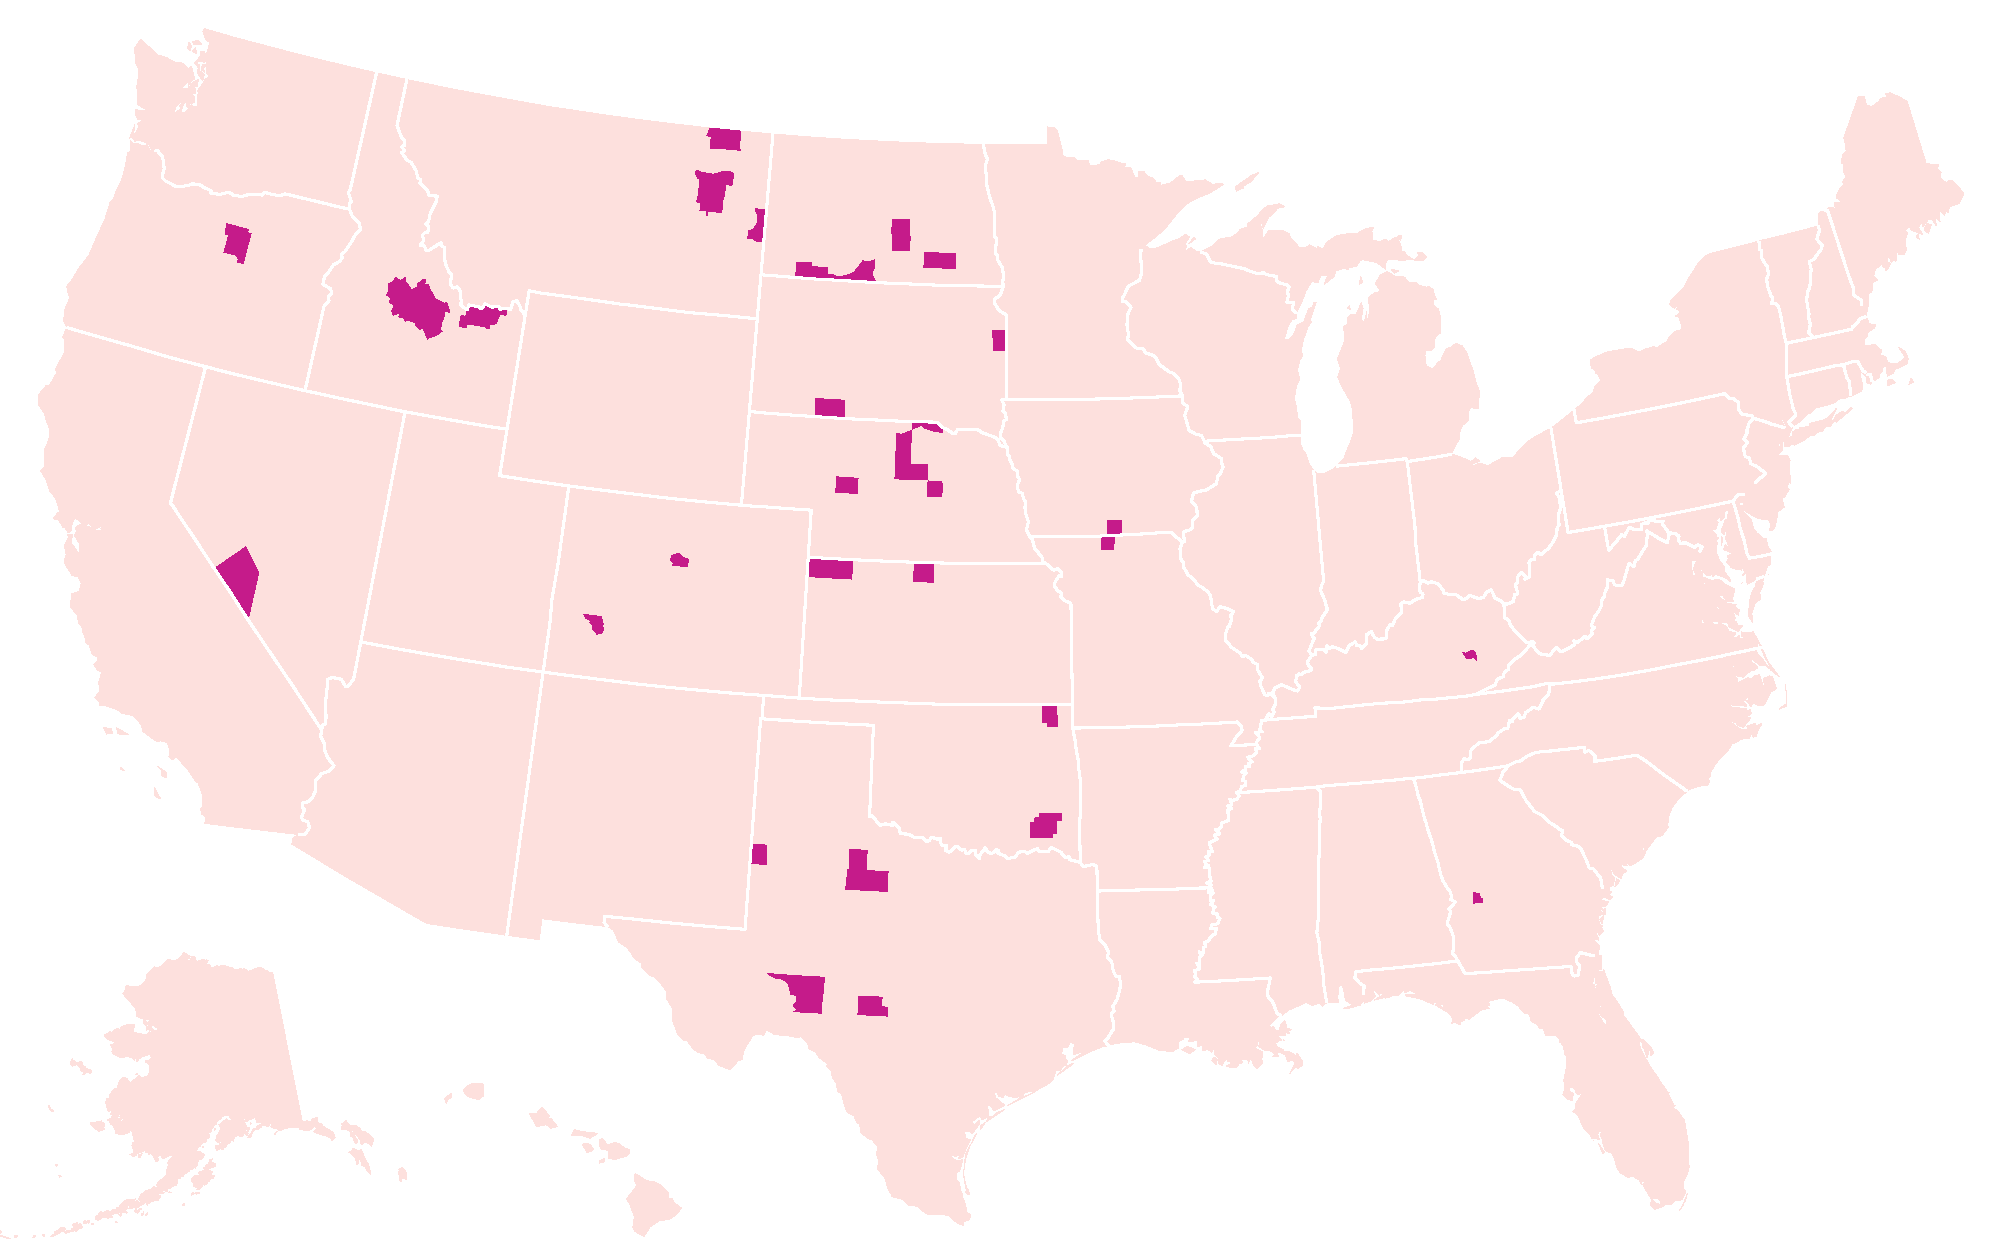
\includegraphics[width=\textwidth]{./figures/poisson-highs}
		\caption{Purple: Bottom 10\% ``Dangerous'' counties.}
		\label{fig:poisson1}
	\end{subfigure}
	~
	\begin{subfigure}[tb]{0.3\textwidth}
		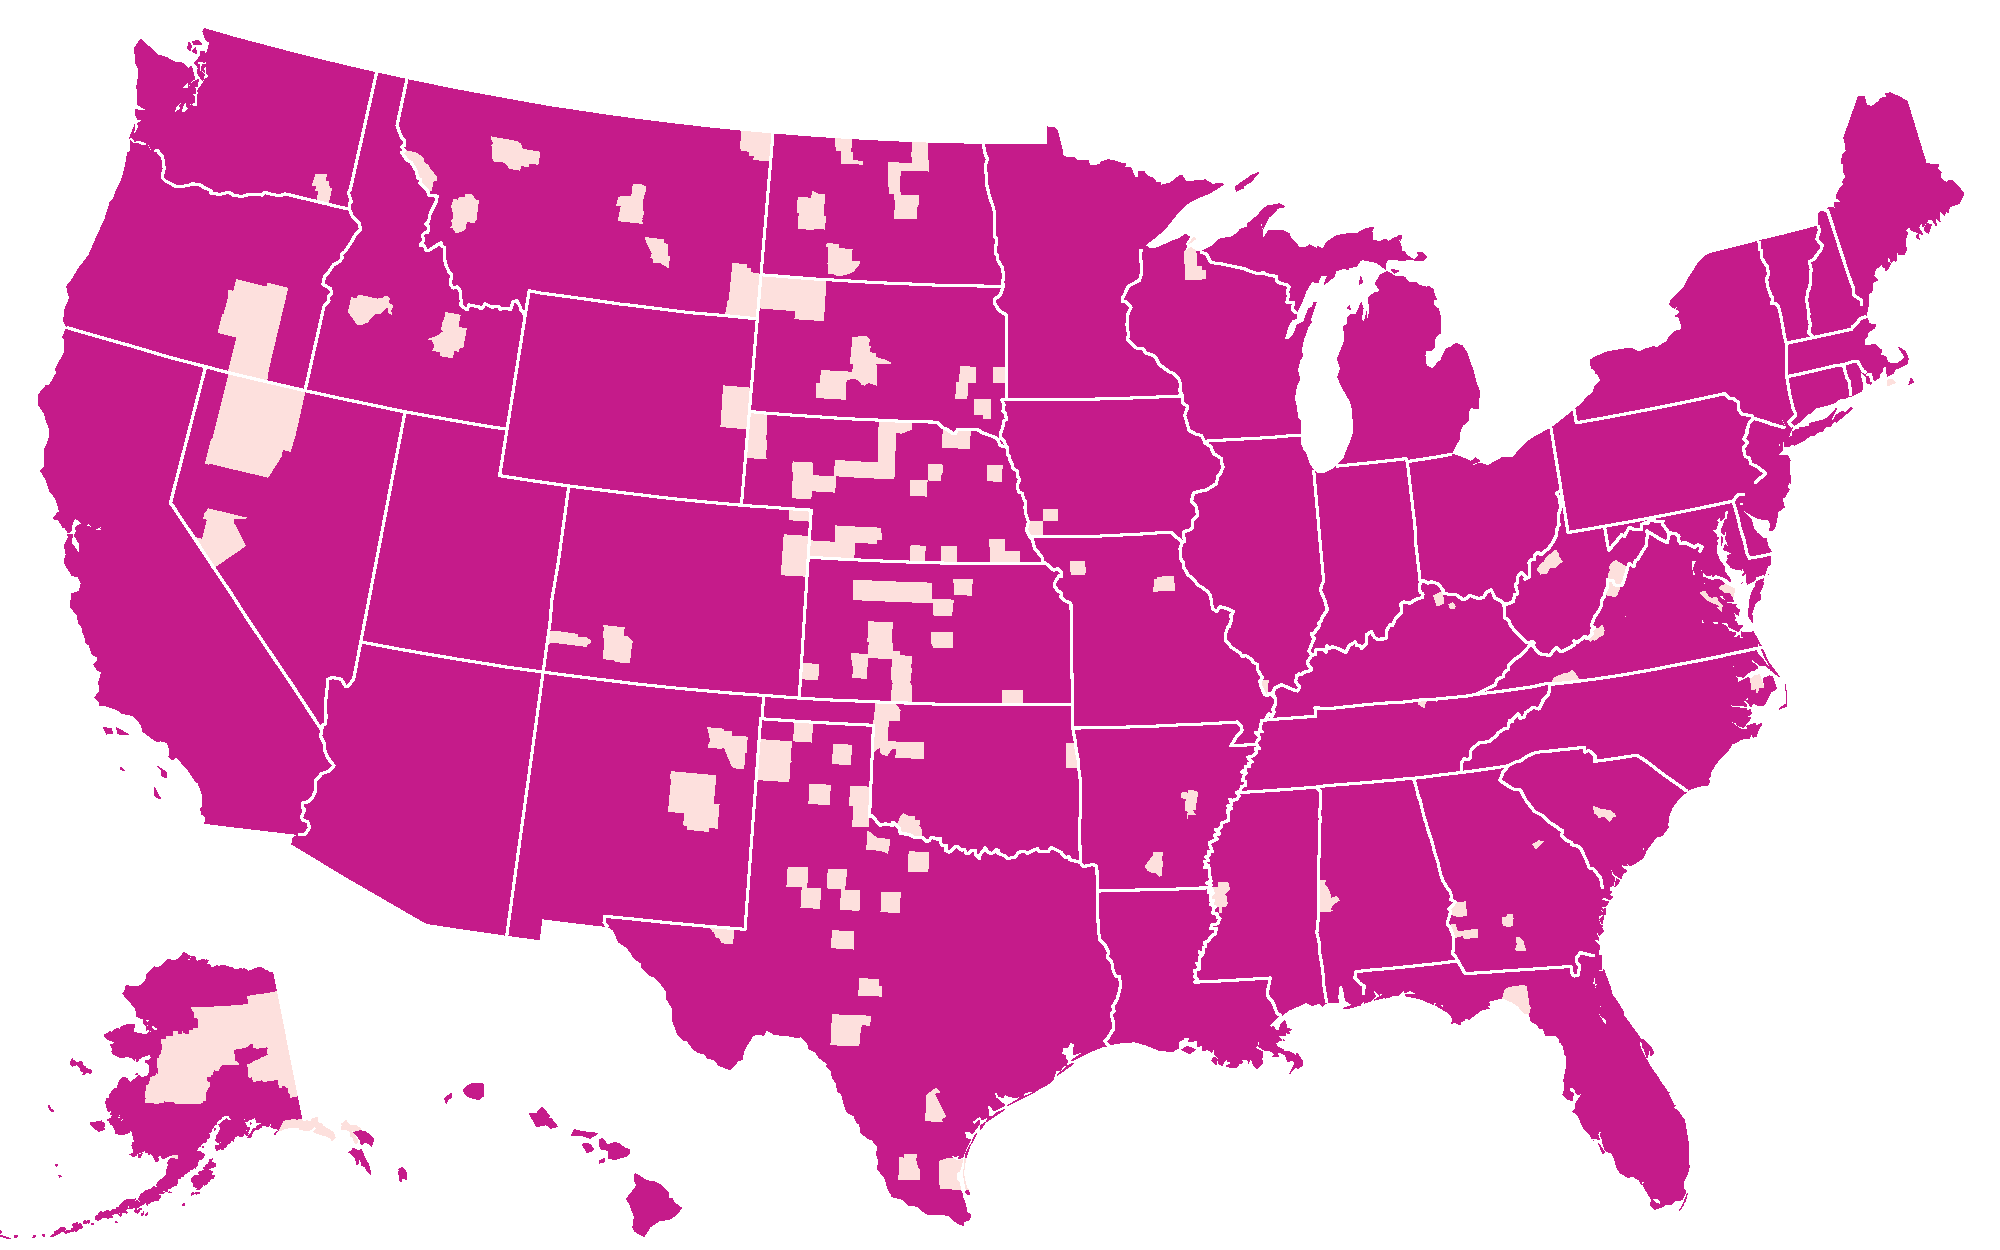
\includegraphics[width=\textwidth]{./figures/poisson-lows}
		\caption{Pink: Top 10\% ``Safe'' counties.}
		\label{fig:poisson2}
	\end{subfigure}
	~
	\begin{subfigure}[tb]{0.3\textwidth}
		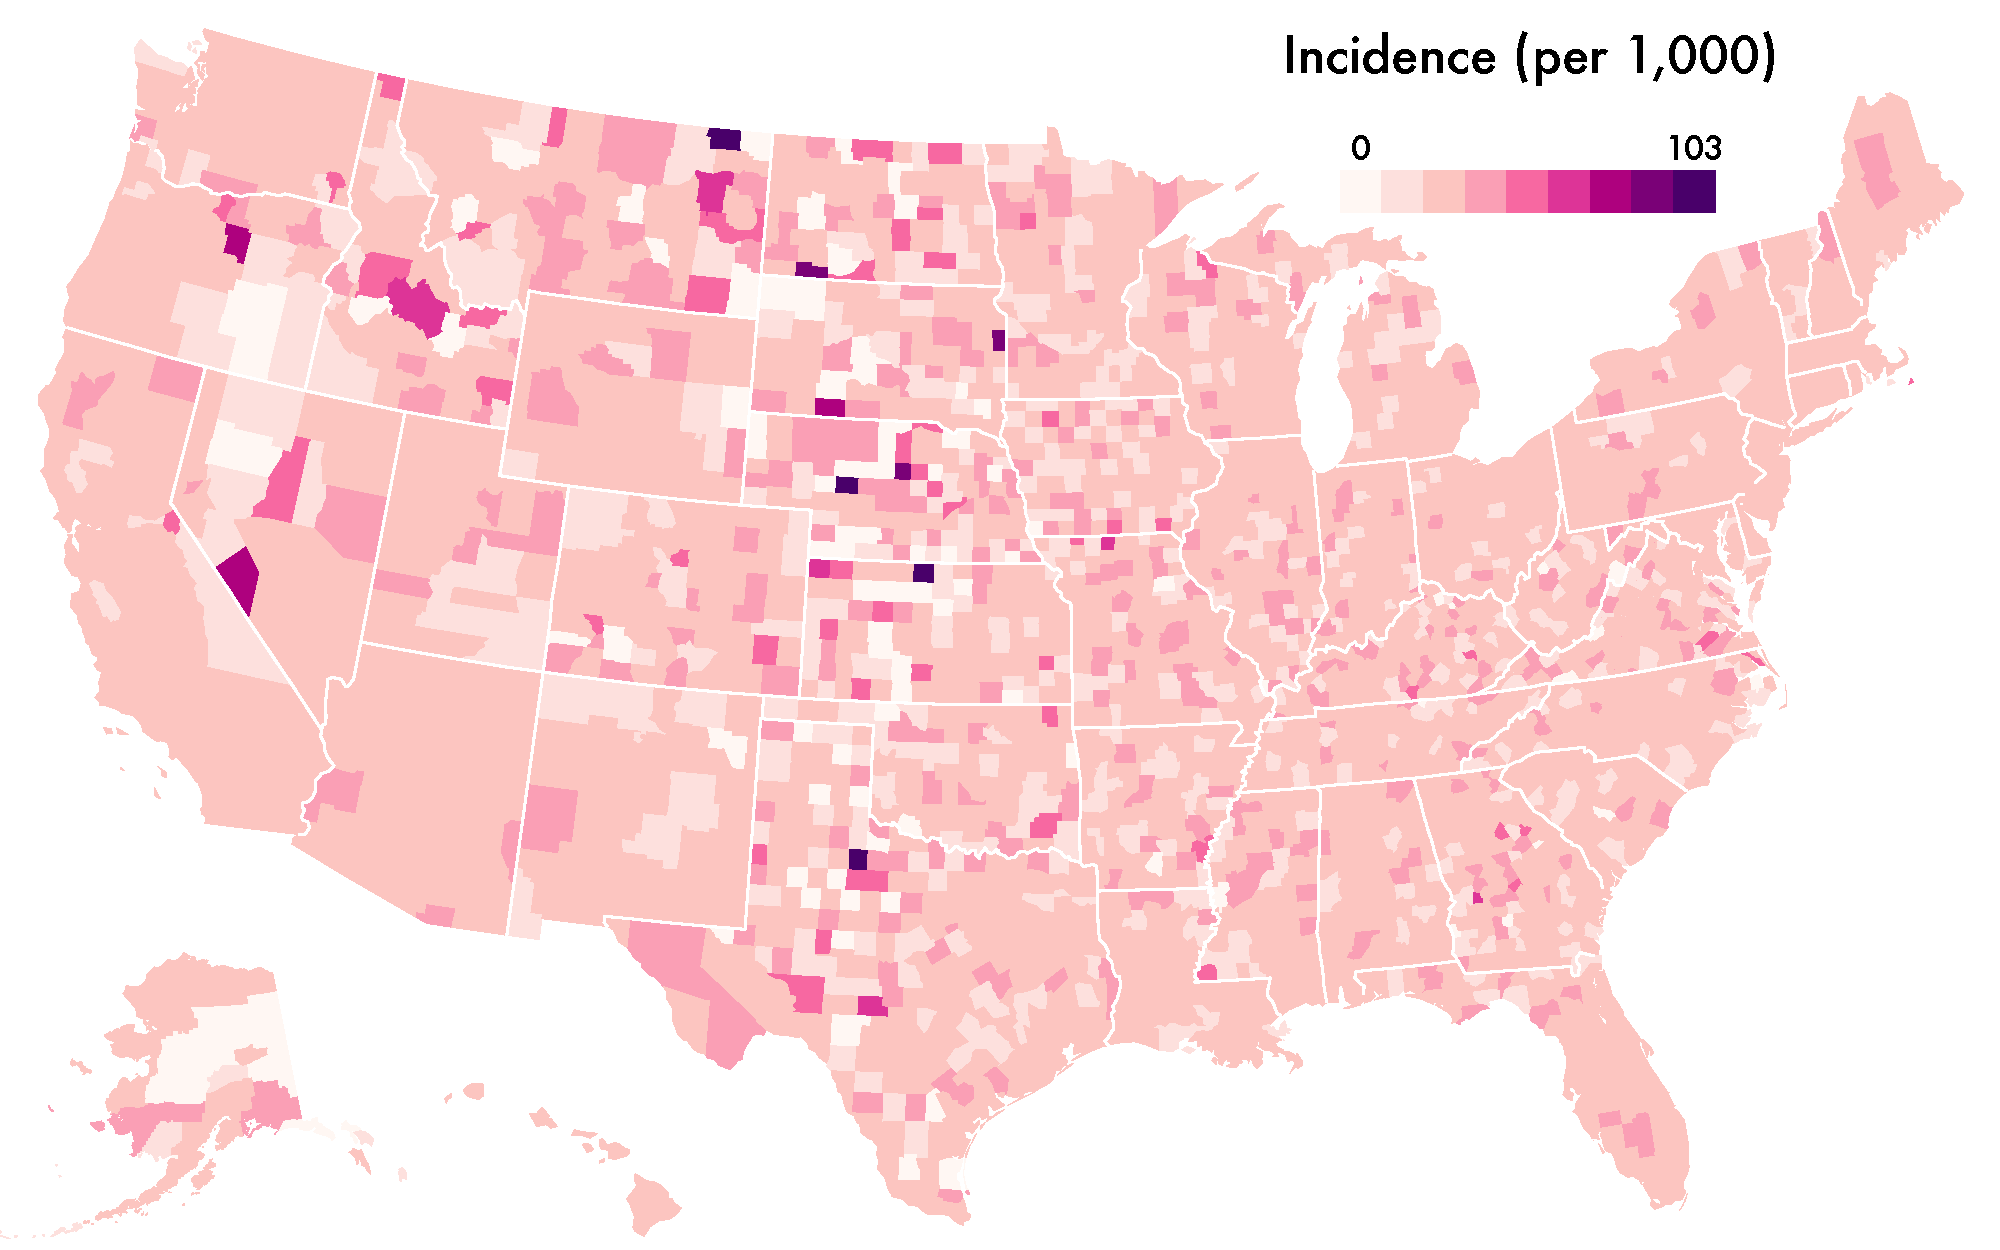
\includegraphics[width=\textwidth]{./figures/poisson}
		\caption{Rates across all counties.}
		\label{fig:poisson3}
	\end{subfigure}
	\caption{Choropleth maps illustrating the sampling error bias. By na\"ively normalizing event density (for instance visualizing per-capita, rather than raw density), latent variables can create erroneous geographic patterns. As an example, low population regions have higher variance than high population regions. These maps encode the per-capita incidence of a fictional disease. (a) The counties with high rates of disease appear localized in the great plains region. However, we also see that (b) the counties with the lowest rates are also mostly located in this region. In fact, the data were generated from a Poisson process with a .1\% chance of infection for each citizen, regardless of location. The apparent geographic patterns are an artifact of (c) the high variance in counties with low population.
	}
	\label{fig:poisson}
\end{figure*}
}

\newcommand{\renormFig}{
\begin{figure*}
	\centering
	\begin{subfigure}[tb]{0.3\textwidth}
		
\includegraphics[width=\textwidth]{./figures/renormc}
		\caption{Initial density map.}
		\label{fig:renorm1}
	\end{subfigure}
	~
	\begin{subfigure}[tb]{0.3\textwidth}
		
\includegraphics[width=\textwidth]{./figures/renorm-modec}
		\caption{Adding to the mode.}
		\label{fig:renorm2}
	\end{subfigure}
	~
	\begin{subfigure}[tb]{0.3\textwidth}
		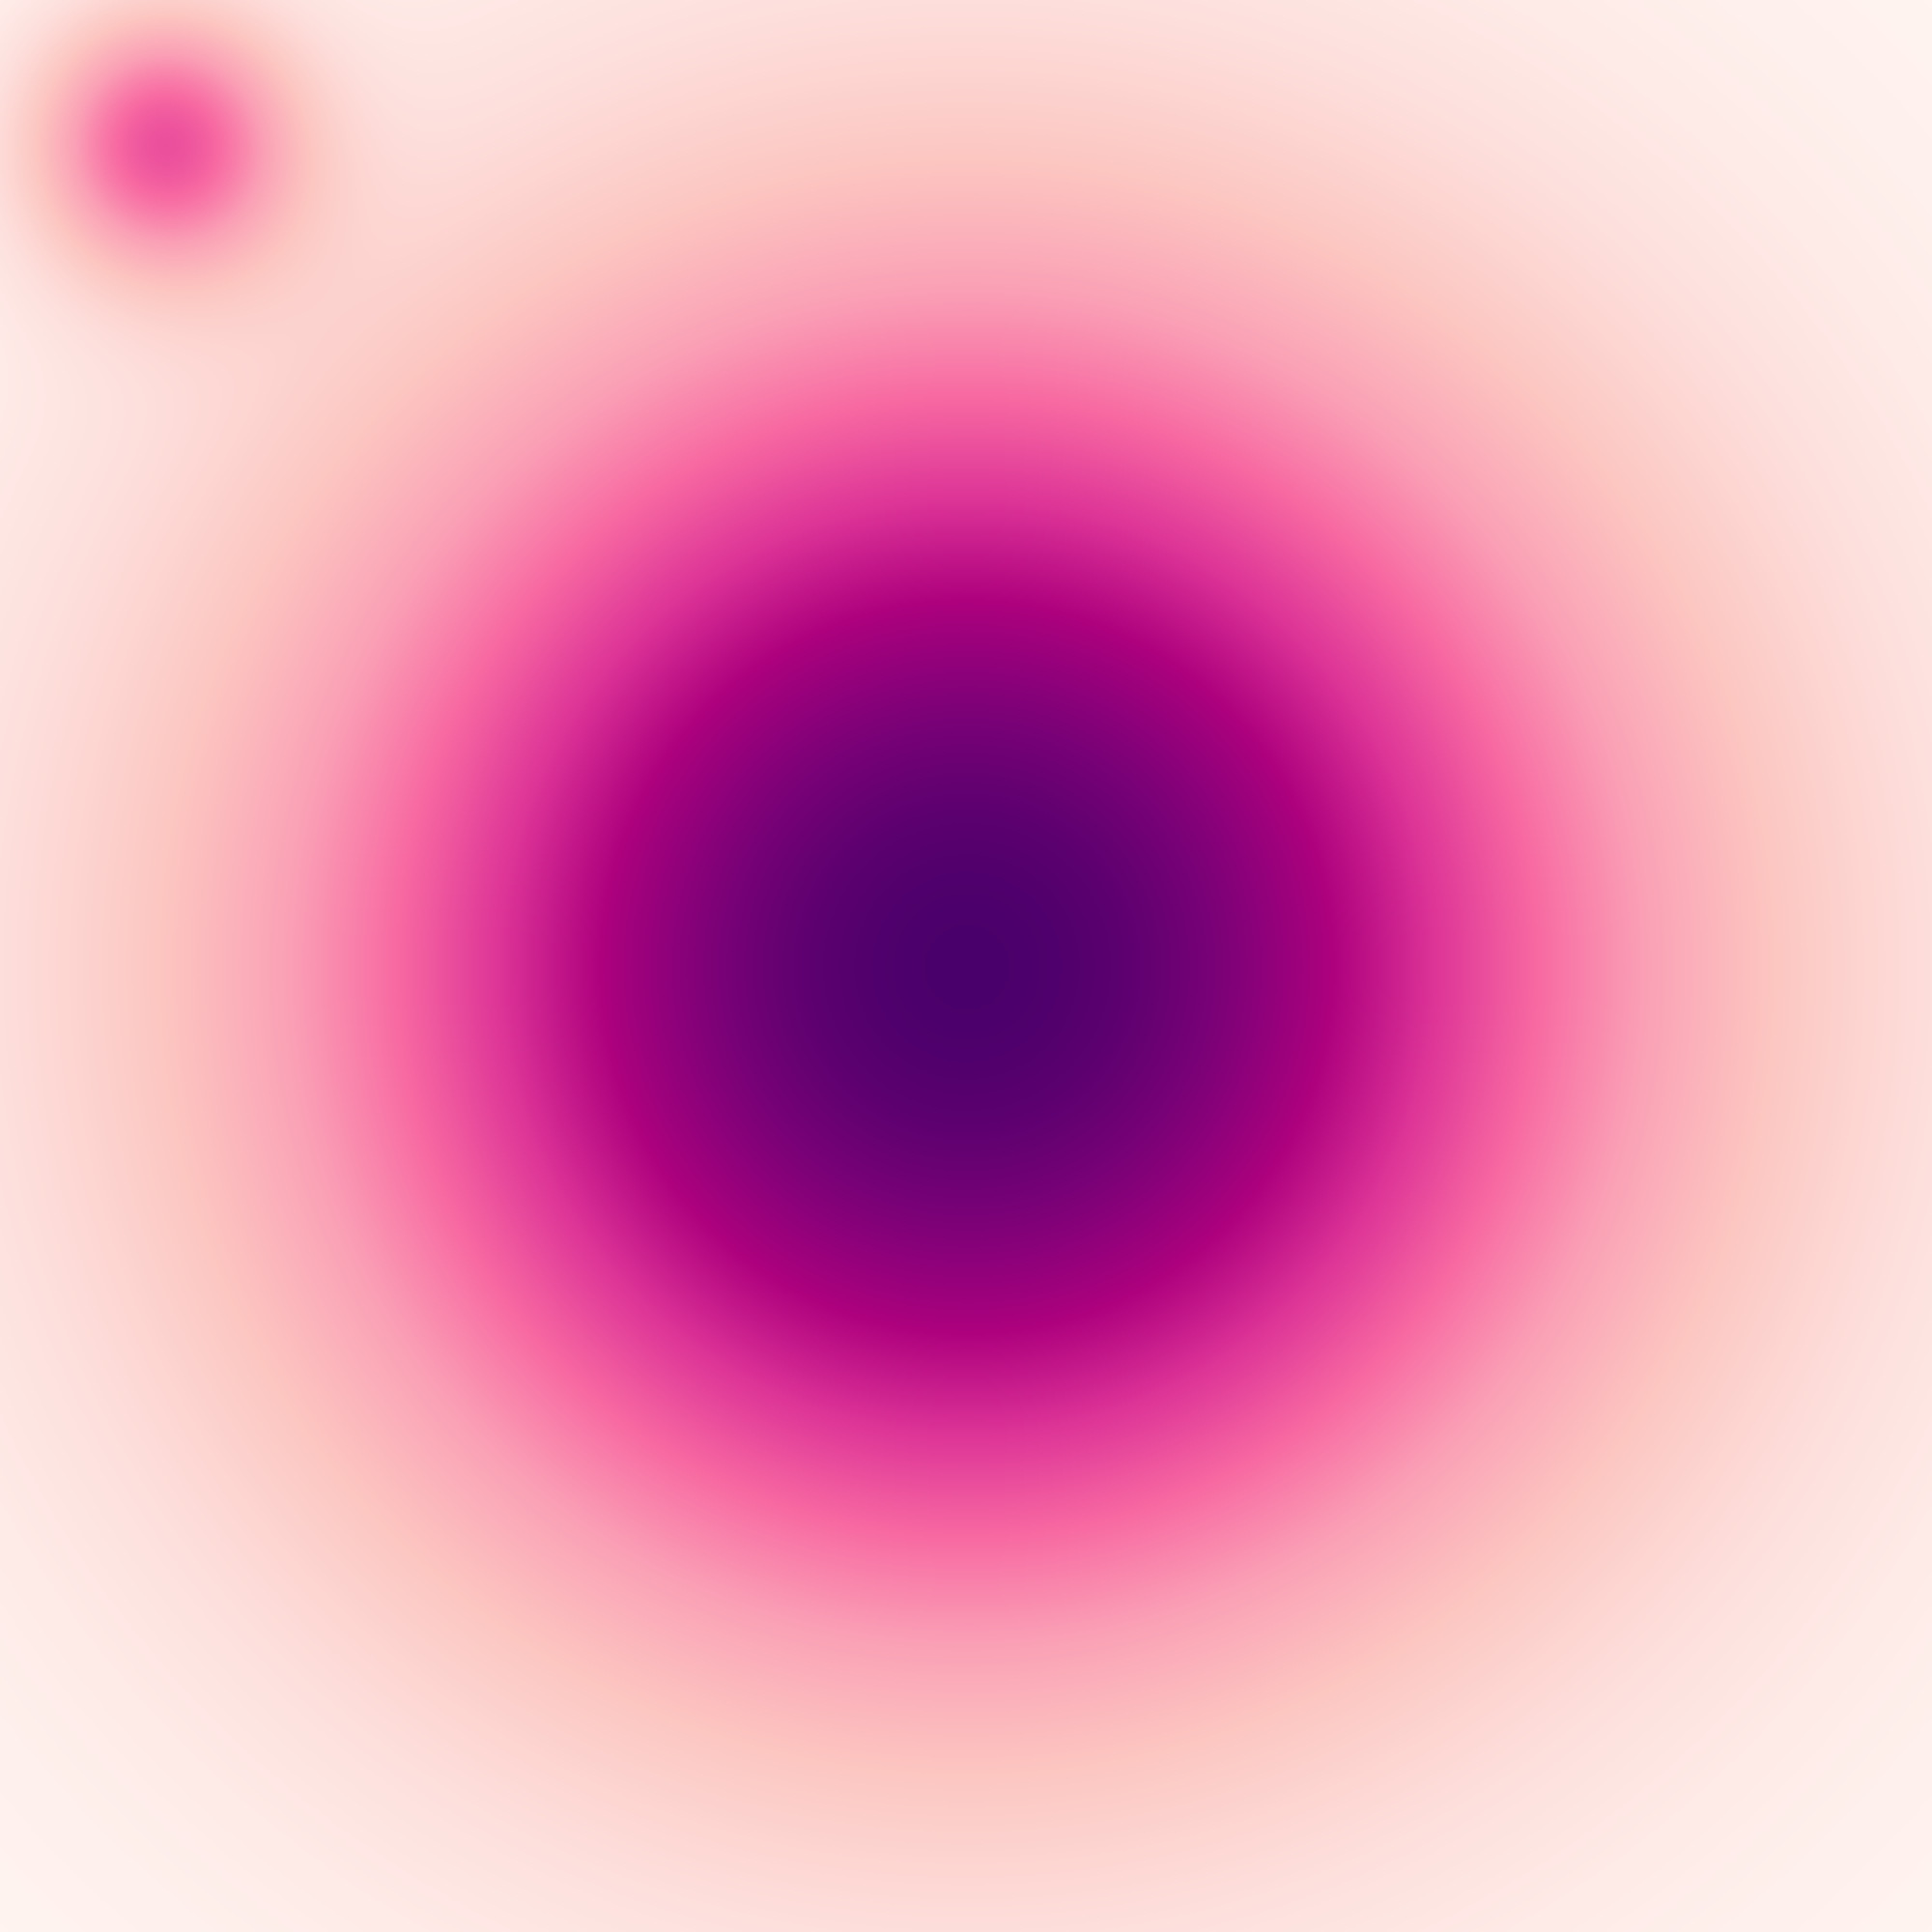
\includegraphics[width=\textwidth]{./figures/renorm-outlierc}
		\caption{Adding an outlier.}
		\label{fig:renorm3}
	\end{subfigure}
	\caption{
		Heatmaps illustrating renormalization bias. Incoming data may force renormalization. This readjustment step can be visually disruptive, even though the event itself may not be. (a) A KDE map of events that are normally distributed. (b) Adding events, represented by a Gaussian kernel, to the modal location causes a large visual change to the resulting density map (over 90\% of pixels have a different color value). (c) Adding outlier events to the upper left (arguably a more significant occurrence), only affects the pixels in the region of the outlier (6\% of pixels).
		%If color is continuously mapped to density, this issue is even more pronounced (99\% vs. 6\% of pixel values changed, depending on color gamut).
	}
	\label{fig:renorm}
\end{figure*}
}


\newcommand{\fireFig}{
	\begin{figure}
		\centering
		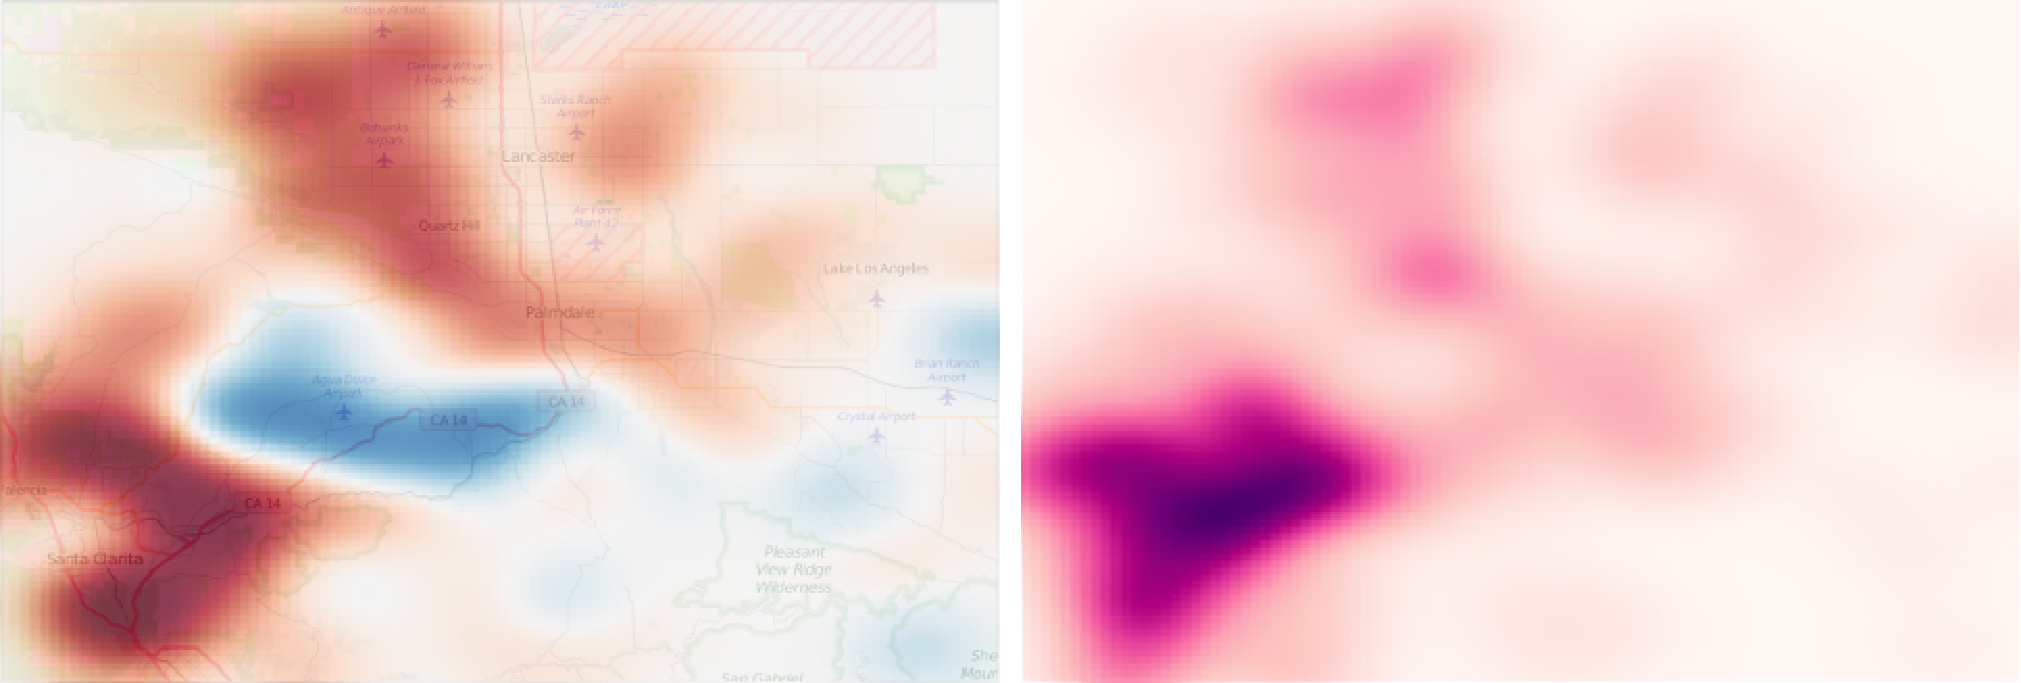
\includegraphics[width=.9\columnwidth]{figures/fire3-2}
		\caption{
			Signed Surprise Map (left) and KDE density map (right) of 313 fires in northern Los Angeles county, from the spacetime package for R \protect\cite{pebesma2012spacetime}. $\mathcal{M}$ consists of Gaussian, uniform, and sampled subset (first 25 fires) models. Signed surprise is on the interval $[-0.53,0.53]$. The sampled subset model quickly becomes the likeliest model (indicating that fires tend to reoccur in similar spatial regions). The first few fires occurred in the far southwest, with isolated fires in regions in the southeast. Over time, this original spatial mode extends slightly southwards. The Surprise Map highlights this new, dangerous region. The faint blue regions in the southeast show locations where fires occurred in the first 25 events, but not subsequently.
		}
		\label{fig:fire}
	\end{figure}
}


%This example is missing something. I've been playing around with having a bunch of bootstrapped models and then seeing what pops out, but the answer is still "not very much, over the 1000 quakes"

\newcommand{\quakeFig}{
	\begin{figure}
		\centering
		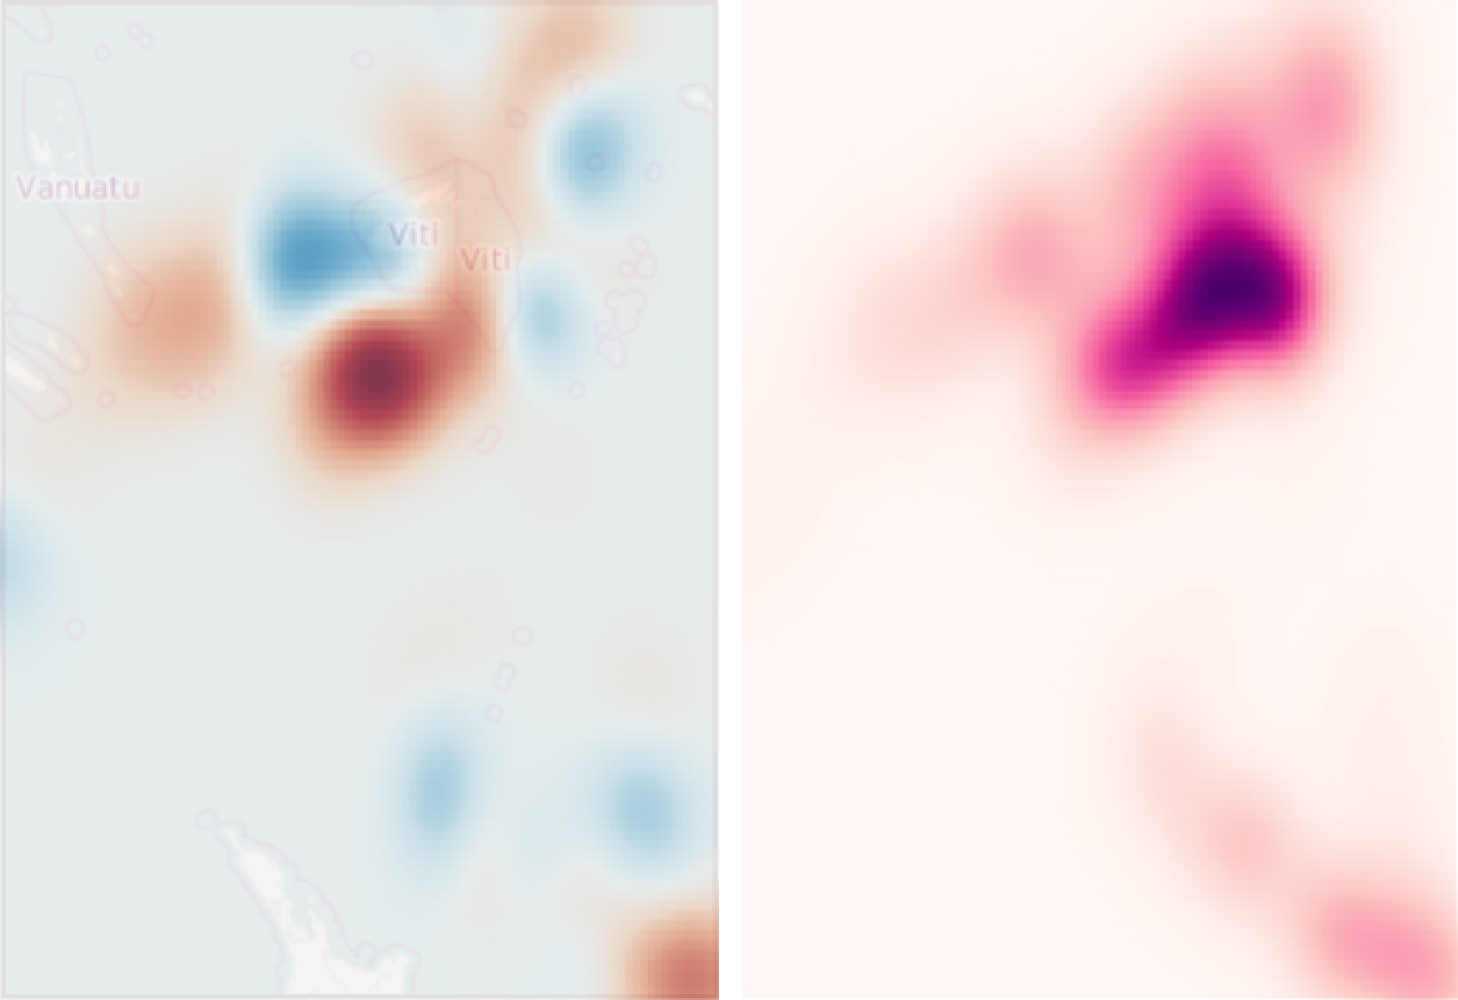
\includegraphics[width=.9\columnwidth]{figures/quake2-2}
		\caption{Signed Surprise Maps (left) and KDE density maps (right) of earthquakes in the South Pacific, near Fiji, from the R datasets package \cite{rdatasets}. $\mathcal{M}$ consists of Gaussian, uniform, and sampled subset (in this case a bootstrapped sample of 50 events) models. Signed surprise is from $[-0.53,0.53]$. The bootstrapped model eventually becomes the most likely, reflecting long-term homogeneity in quake location. However, small differences in density (such as the red region south of Fiji with higher than expected quake density), are highlighted in the Surprise maps, allowing more focused comparison across timepoints.
		}
		\label{fig:quake}
	\end{figure}
}

\newcommand{\quakeFigvTwo}{
	\begin{figure}[htb]
		\centering
		\begin{subfigure}[t]{.35\textwidth}
			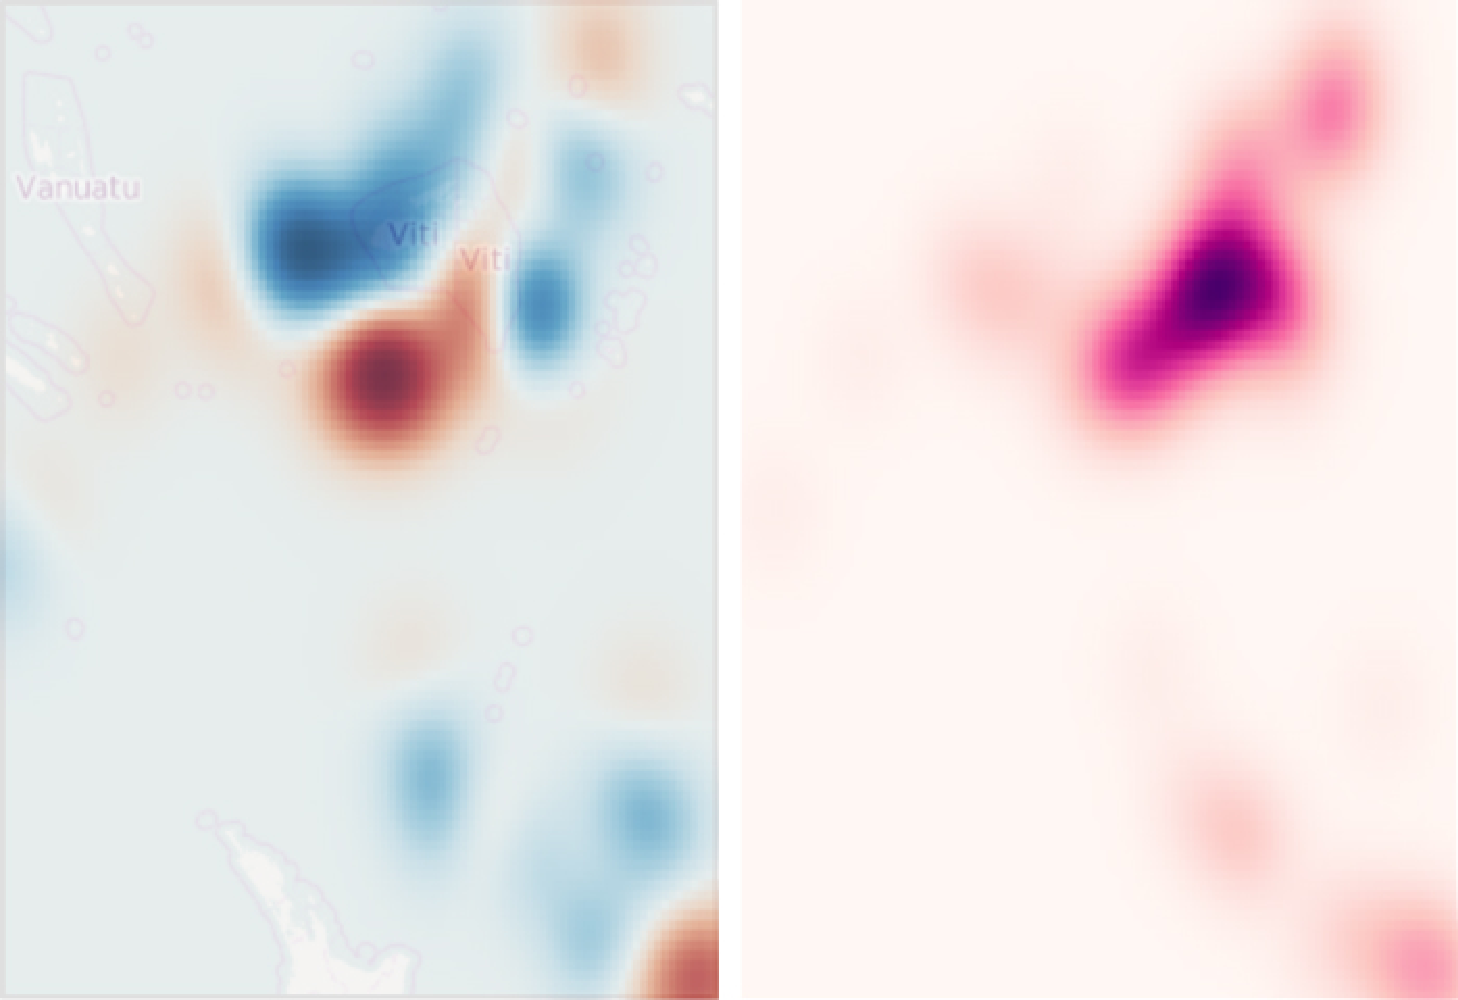
\includegraphics[width=\textwidth]{figures/quake1-2}
			\caption{Signed Surprise and KDE Density after 100 events. }
			\label{fig:quake2-1}
		\end{subfigure}

		\begin{subfigure}[t]{.35\textwidth}
			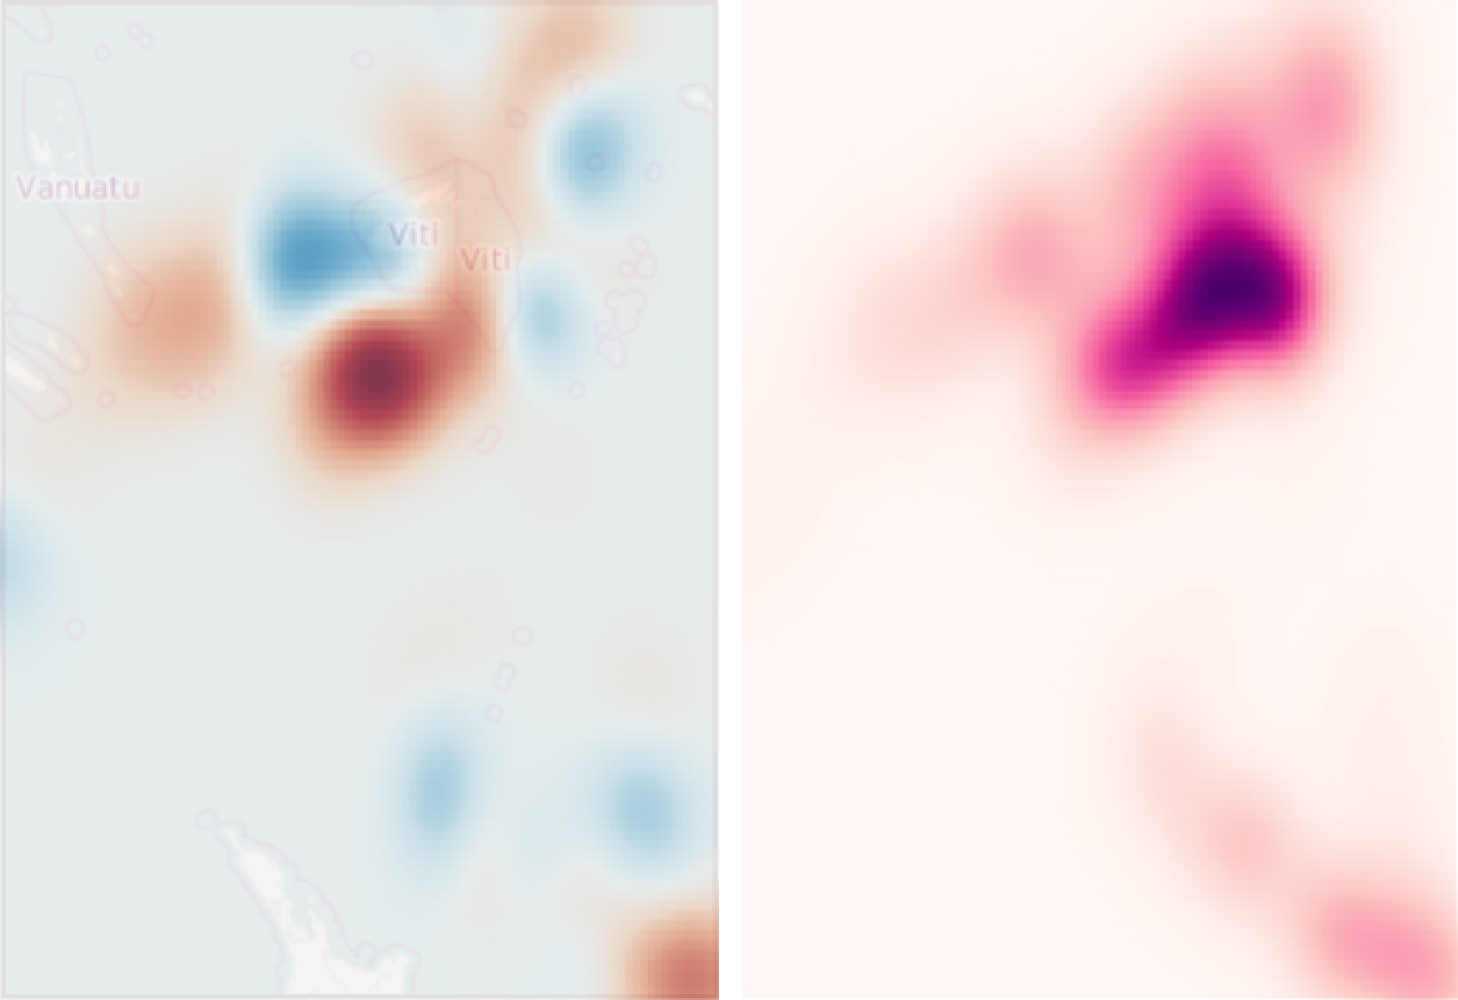
\includegraphics[width=\textwidth]{figures/quake2-2}
			\caption{Signed Surprise and KDE Density after 1,000 events.}
			\label{fig:quake2-2}
		\end{subfigure}

		\caption{Signed Surprise Maps (1st and 3rd from left) and KDE density maps (2nd and 4th from left) of earthquakes in the South Pacific, near Fiji, from the R datasets package \cite{rdatasets}, after 100 (Fig. \ref{fig:quake2-1}) and 1,000 (Fig. \ref{fig:quake2-2}) events. $\mathcal{M}$ consists of Gaussian, uniform, and sampled subset (in this case a bootstrapped sample of 50 events) models. Signed surprise is from $[-0.53,0.53]$. The bootstrapped model eventually becomes the most likely, reflecting long-term homogeneity in quake location. This homogeneity makes it difficult to compare densities using a traditional KDE map. Bootstrapped models afford comparison to a sampled representation of the whole, highlighting differences such as the underrepresentation of northern quakes after 100 events.
		}
		\label{fig:quake2}
	\end{figure}
}


\newcommand{\unemploymentFig}{
	\begin{figure}
		\centering
		\begin{subfigure}[t]{.9\columnwidth}
			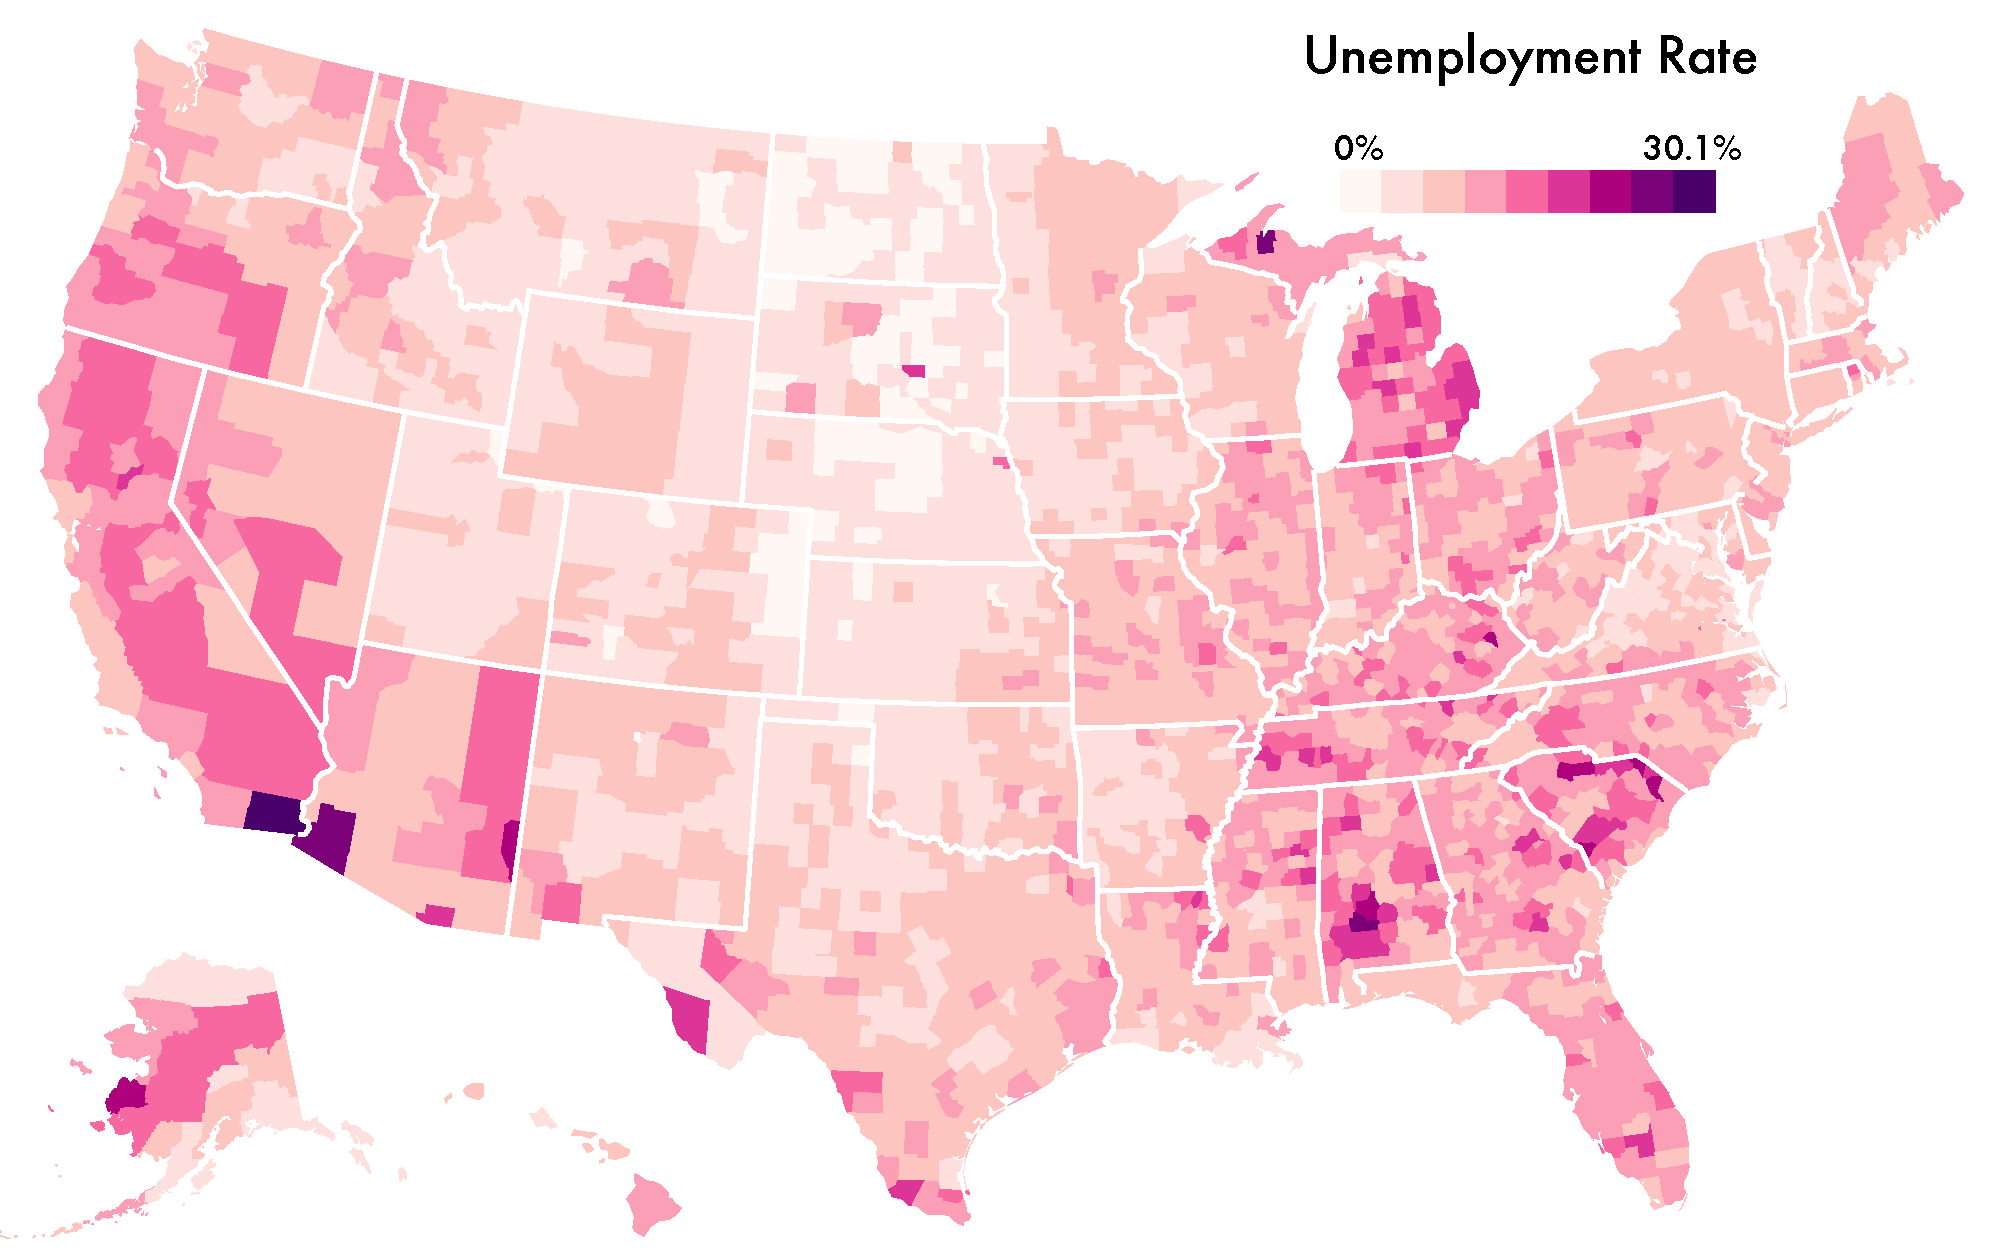
\includegraphics[width=\textwidth]{figures/unemployment2}
			\caption{Per capita event rate map. }
			\label{fig:unemployment1}
		\end{subfigure}

		\begin{subfigure}[t]{.9\columnwidth}
			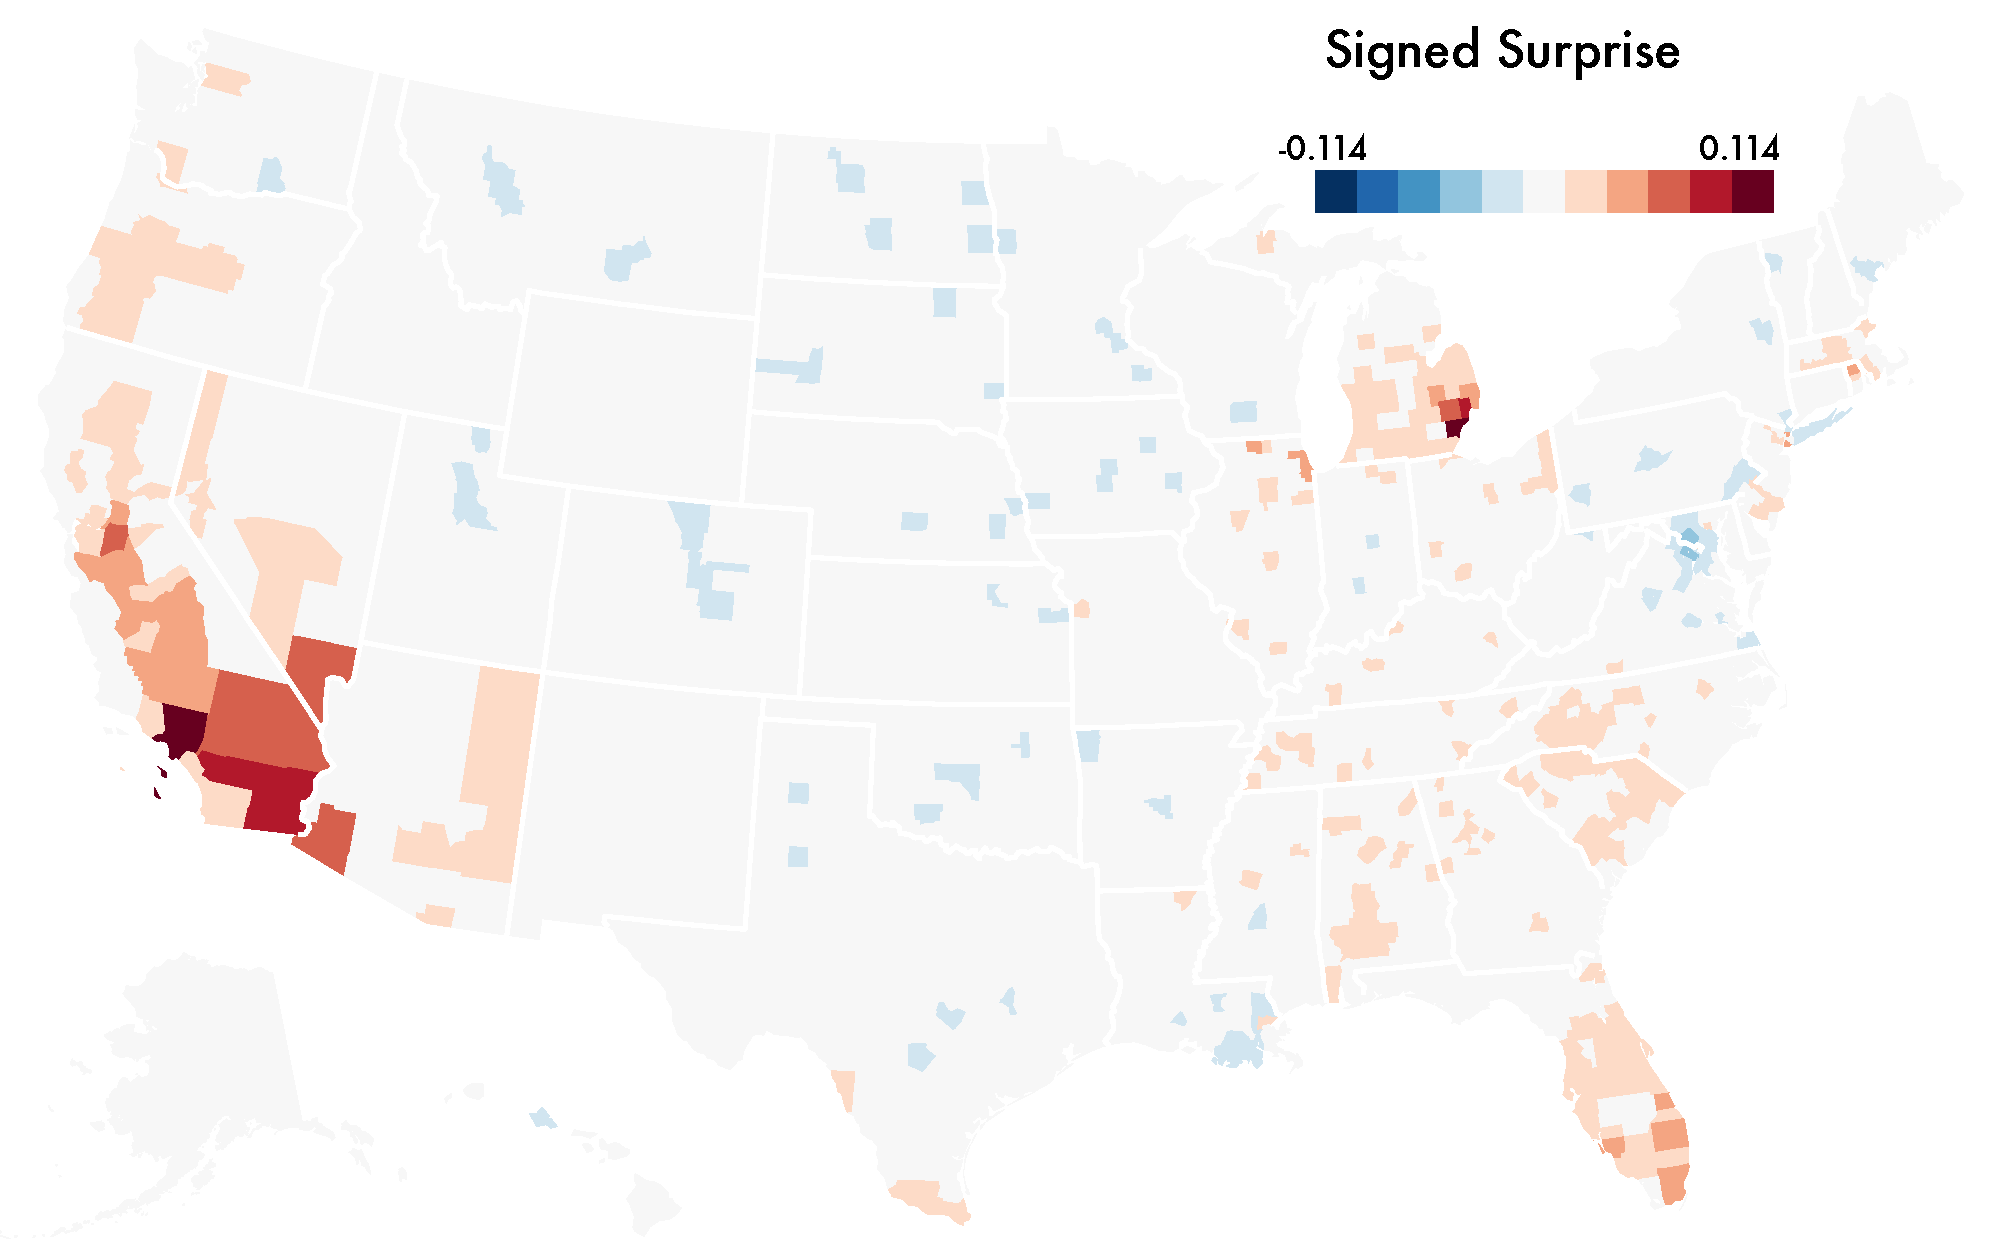
\includegraphics[width=\textwidth]{figures/unemployment-surprise}
			\caption{Signed Surprise Map. }
			\label{fig:unemployment2}
		\end{subfigure}
		\caption{Comparing a traditional map of the 2008 per-capita unemployment rate (Fig. \protect\ref{fig:unemployment1}) with a Surprise Map (Fig. \protect\ref{fig:unemployment2}). $\mathcal{M}$ is a population model and a de Moivre funnel (see Fig. \protect\ref{fig:funnel}) for details. The traditional map seems to show that the great plains region has particularly low unemployment, but the low populations in these regions make those data unreliable. Down-weighting sparse counties with high variance, the Surprise Map shows robustly high unemployment in the Los Angeles and the Detroit metro areas. The Washington D.C. metro area has surprisingly low unemployment, perhaps due to the many jobs provided by the Federal government and related agencies.
		}
		\label{fig:unemployment}
	\end{figure}
}

\newcommand{\coasstFig}{
	\begin{figure*}
		\centering
		\begin{subfigure}[t]{.3\textwidth}
			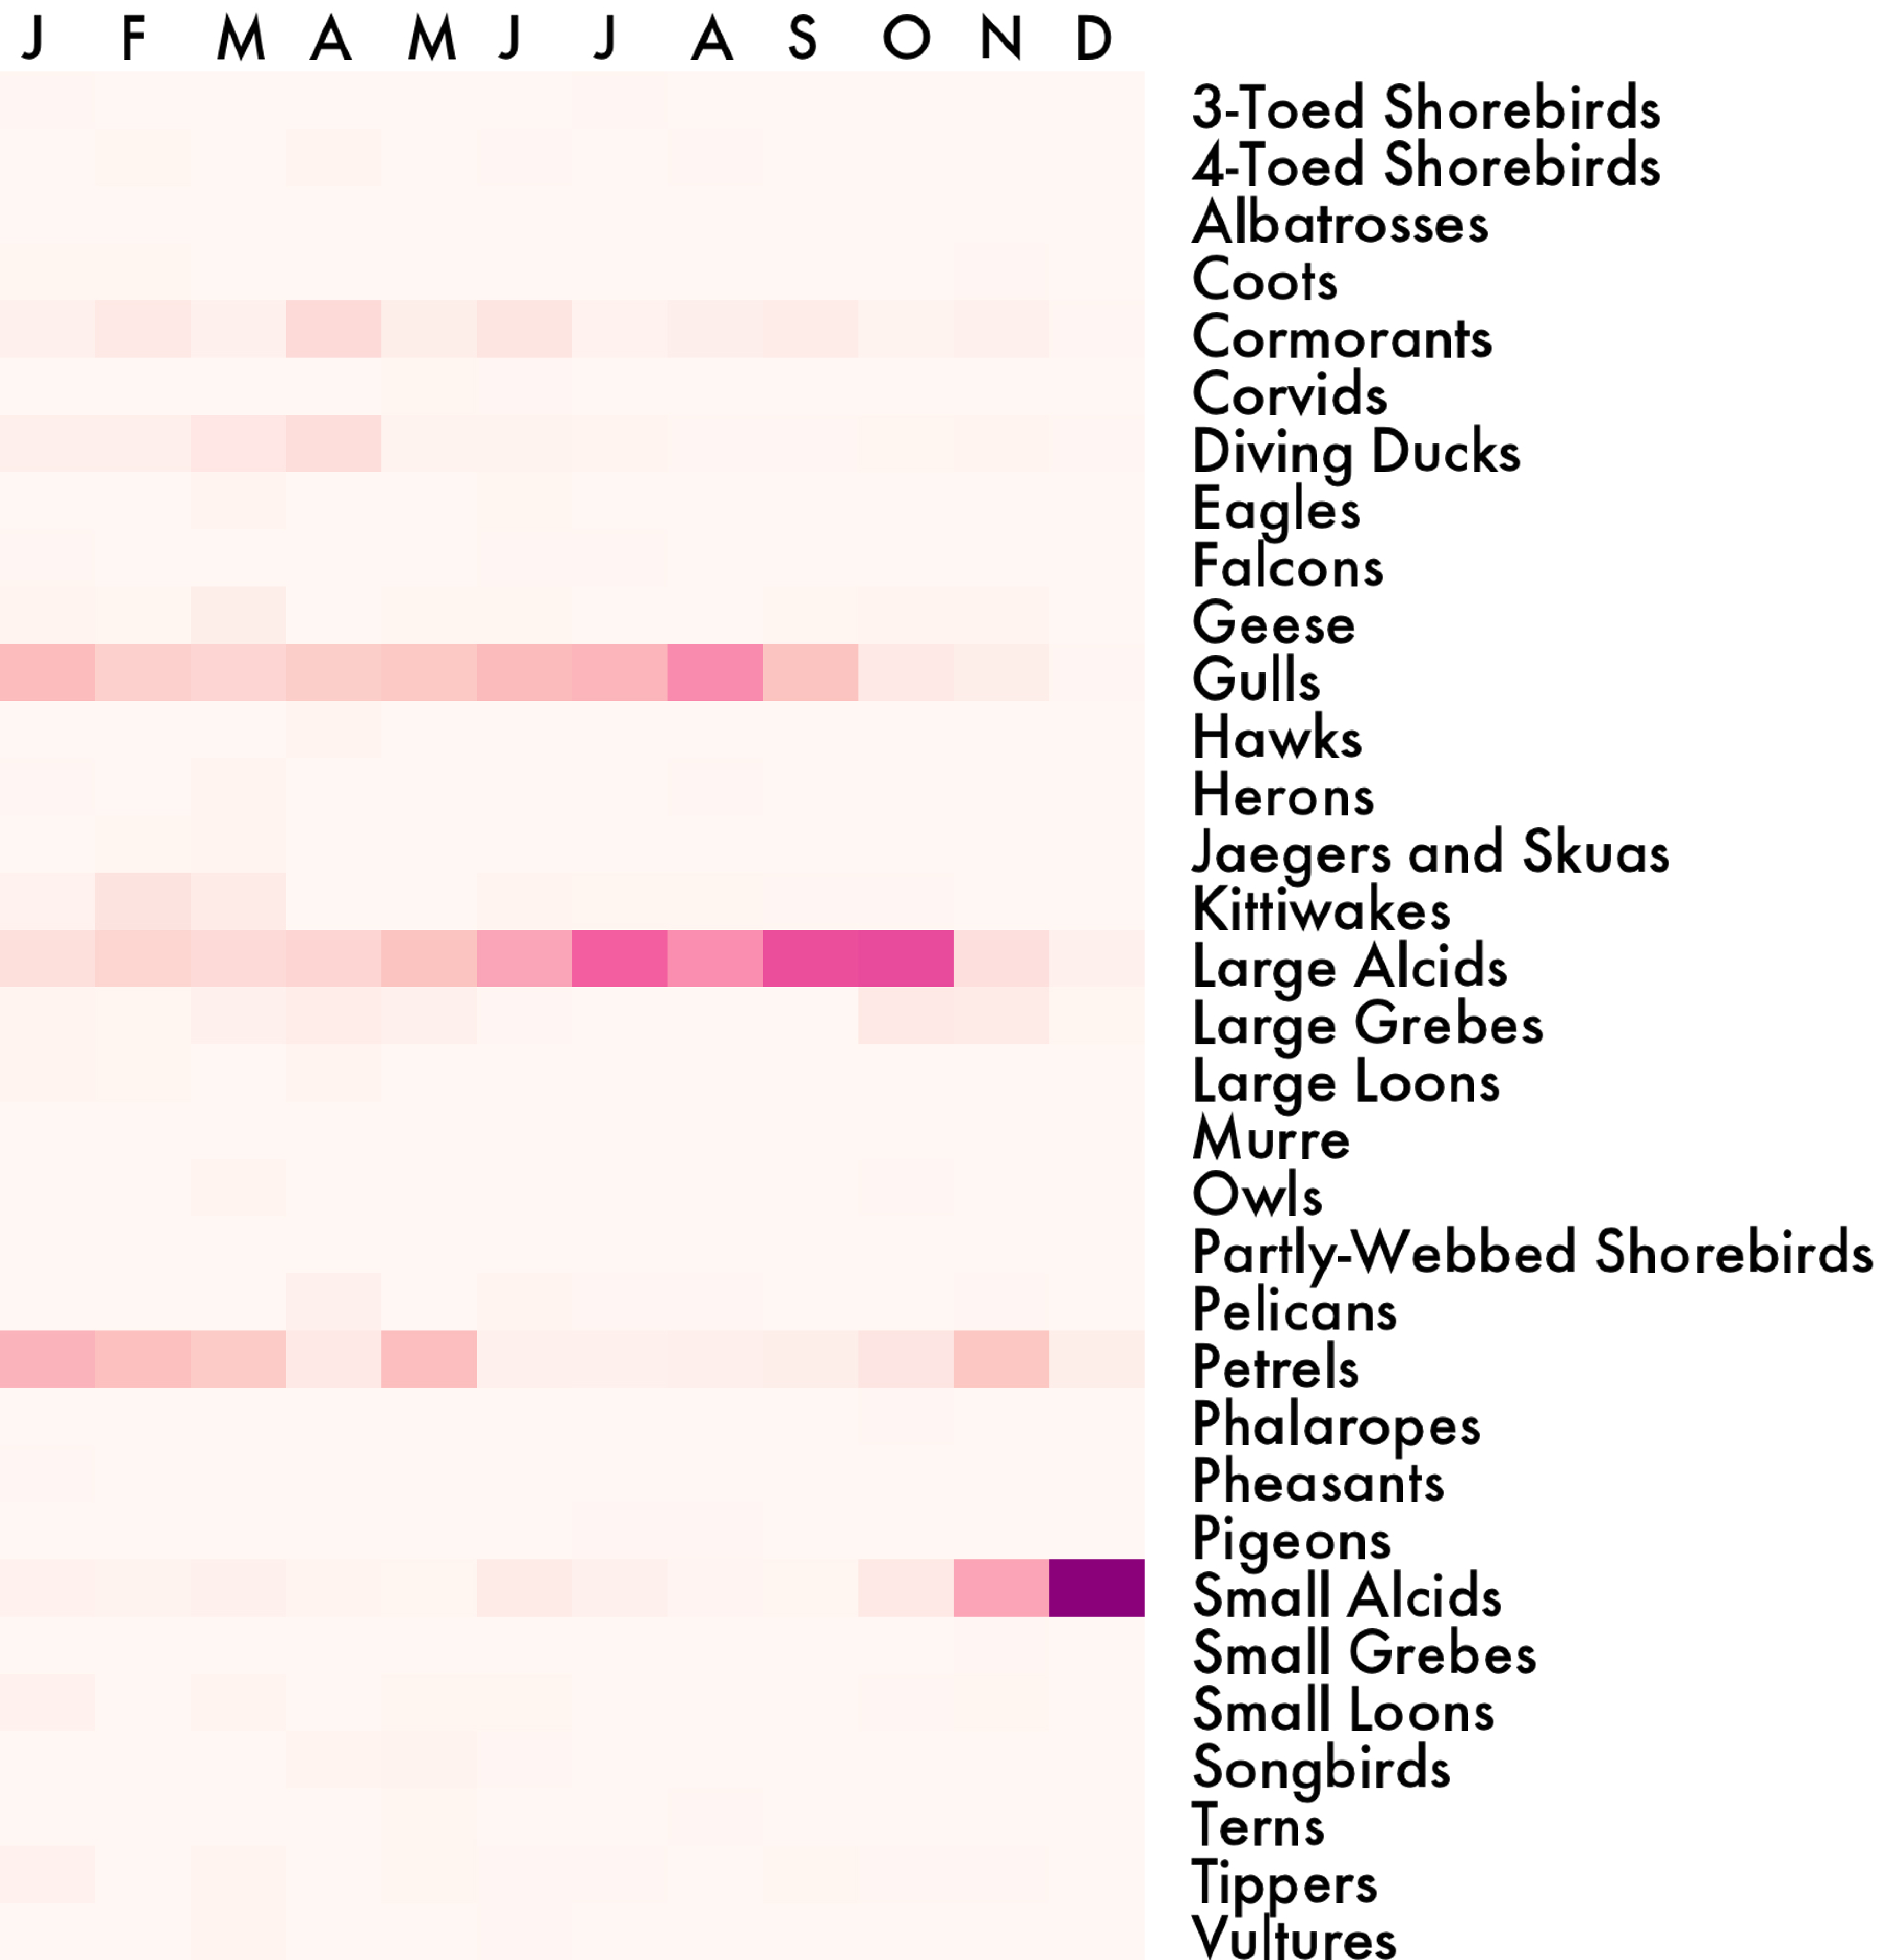
\includegraphics[width=\textwidth]{figures/coasst-observed}
			\caption{Bird death event rate map. }
			\label{fig:coasst1}
		\end{subfigure}
		~
		\begin{subfigure}[t]{.3\textwidth}
		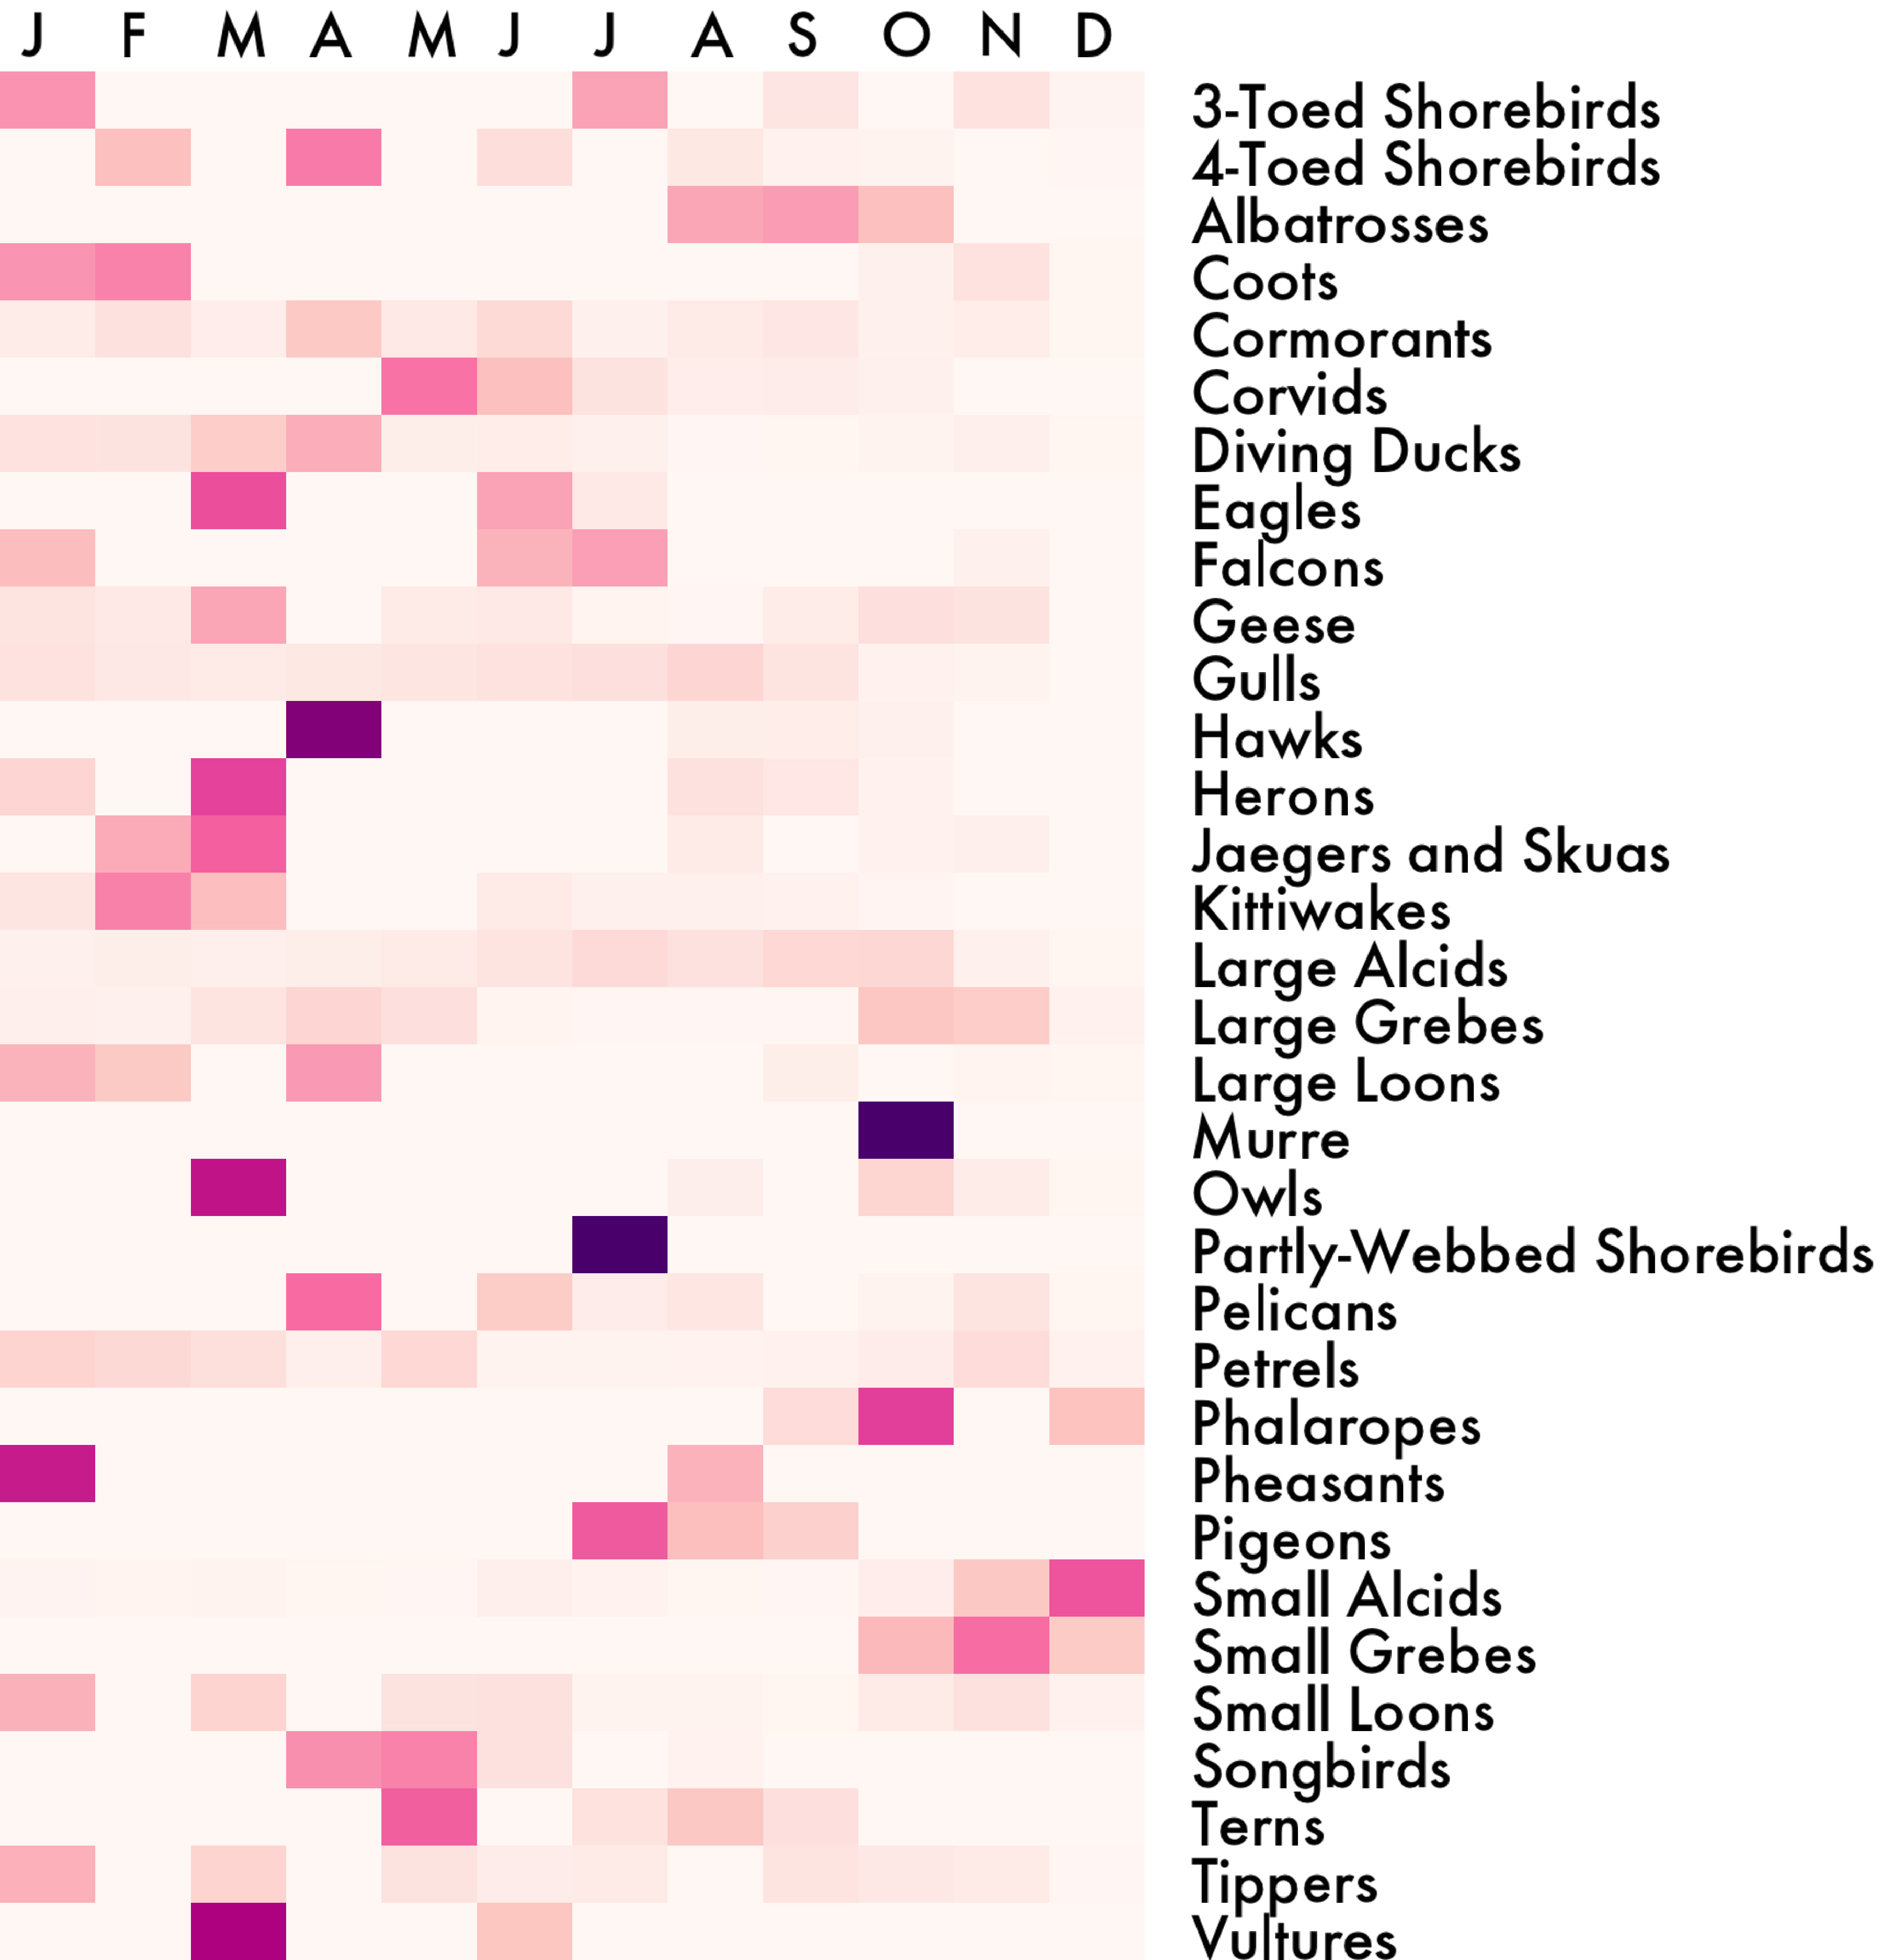
\includegraphics[width=\textwidth]{figures/coasst-normalized}
		\caption{Per species normalized bird death map. }
		\label{fig:coasstn}
		\end{subfigure}
		~
		\begin{subfigure}[t]{.3\textwidth}
			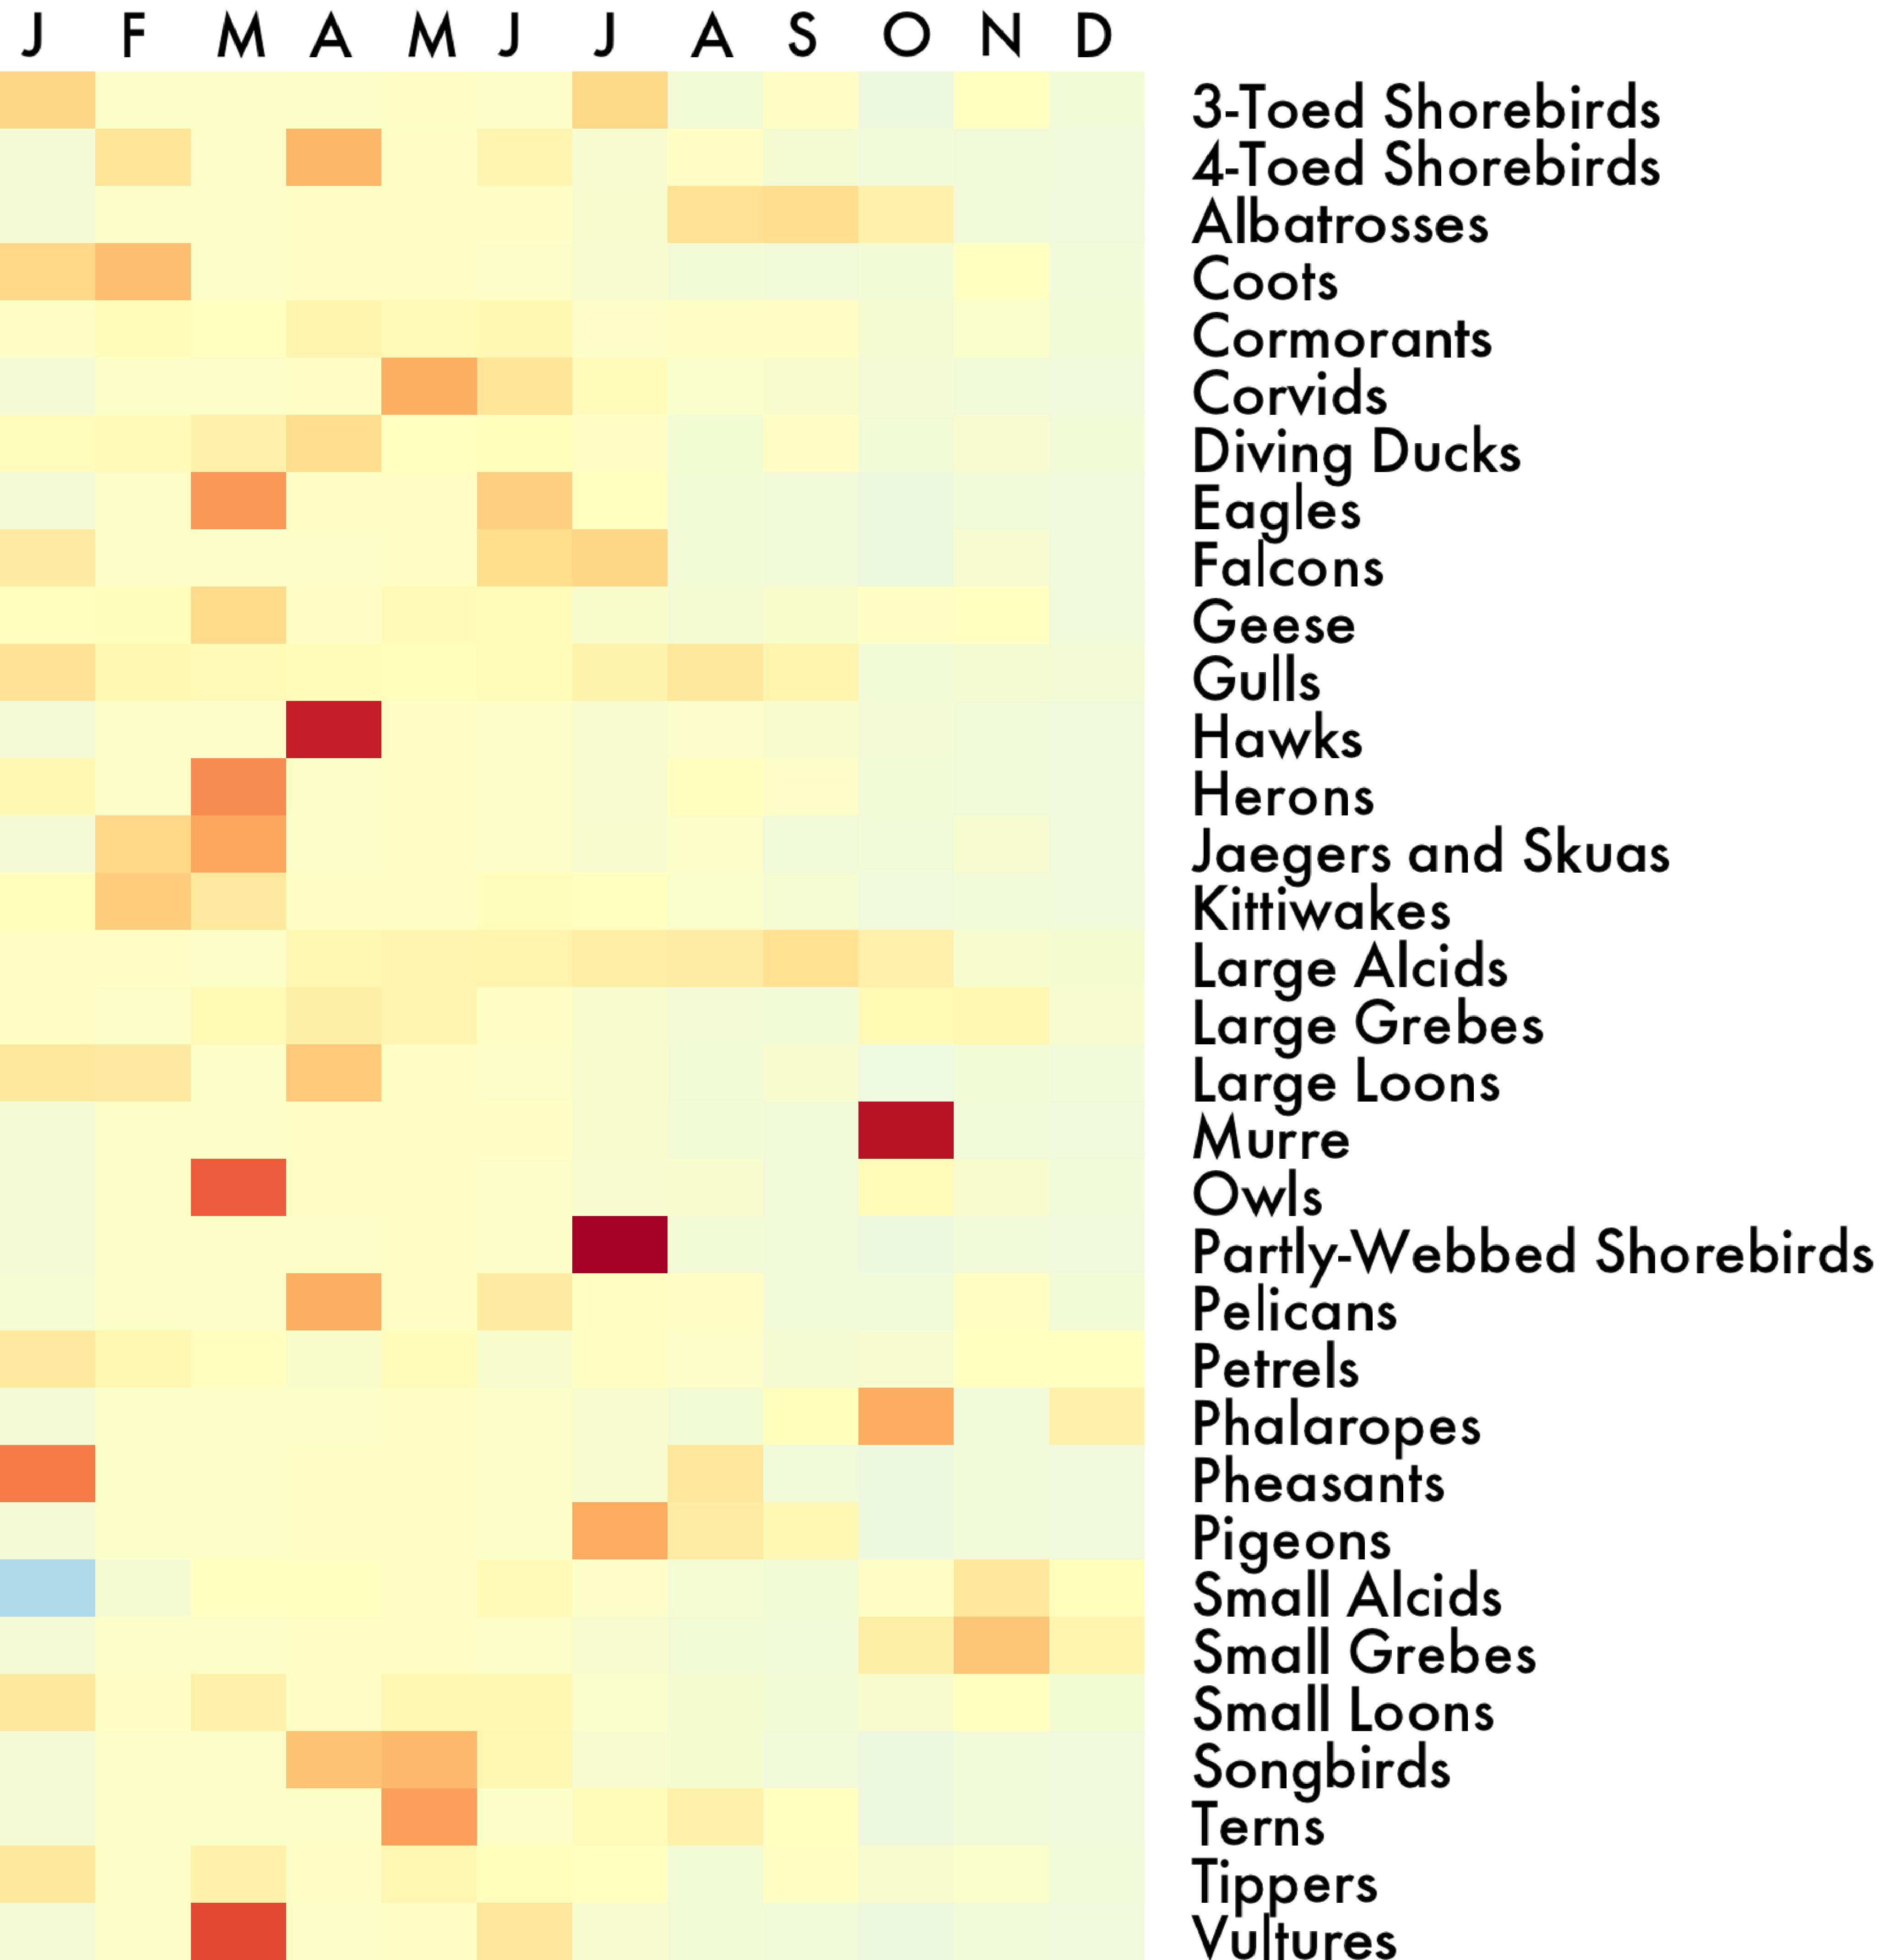
\includegraphics[width=\textwidth]{figures/coasst-surprise}
			\caption{Signed Surprise Map. }
			\label{fig:coasst2}
		\end{subfigure}
		\caption{Comparing event density (Fig. \protect\ref{fig:coasst1}) and event rate (Fig. \protect\ref{fig:coasstn}) maps of 2014 per-species surveyed bird deaths  with a Surprise Map (Fig. \protect\ref{fig:coasst2}). Data comes from the COASST beached bird dataset \protect\cite{coasst}. $\mathcal{M}$ is a population model based on data from 1999-2015, and a seasonal model based on per-month variation. Signed surprise is from $[-0.9,0.9]$. Common species families like gulls and alcids (puffins) dominate the density map, making it difficult to reason about non-modal species. The normalized rate map allows analysts to better distinguish intra-species patterns, but hides deviations from seasonal patterns, such as the uncommonly low death rate of Small Alcids in January (0.15\% of all 2014 Small Alcid deaths): normally, 40.56\% of Small Alcid deaths occur in January.
		}
		\label{fig:coasst}
	\end{figure*}
}
%% Uncomment below to include a teaser figure.
 \teaserFig


%% Uncomment below to disable the manuscript note
%\renewcommand{\manuscriptnotetxt}{}

%% Copyright space is enabled by default as required by guidelines.
%% It is disabled by the 'review' option or via the following command:
% \nocopyrightspace

%%%%%%%%%%%%%%%%%%%%%%%%%%%%%%%%%%%%%%%%%%%%%%%%%%%%%%%%%%%%%%%%
%%%%%%%%%%%%%%%%%%%%%% START OF THE PAPER %%%%%%%%%%%%%%%%%%%%%%
%%%%%%%%%%%%%%%%%%%%%%%%%%%%%%%%%%%%%%%%%%%%%%%%%%%%%%%%%%%%%%%%%

\begin{document}

%% The ``\maketitle'' command must be the first command after the
%% ``\begin{document}'' command. It prepares and prints the title block.

%% the only exception to this rule is the \firstsection command
\firstsection{Introduction}

\maketitle

%% \section{Introduction} %for journal use above \firstsection{..} instead


% Things to remember:
% This is a technique paper, not a system paper! We should maybe talk a little about computational complexity, but we should neither promise nor attempt to deliver anything more
% "engineered" than a software interface

There is only limited utility in seeing the expected. In the process of data analysis, one often seeks out outliers and oddities, places where the data do not match our expectations. Unexpected events or patterns of events can occur in time, space, or a combination of both. Spatial event data is often visualized using thematic maps. However, these maps are sensitive to both base rates and sampling error, but rarely explicitly encode information about either. As a result, such maps may \emph{obscure} unexpected but important patterns, or \emph{mislead} the viewer into thinking an important pattern exists, when noise or sampling error are likelier explanations.

In order to address the potential drawbacks of standard thematic maps, we adapt a saliency technique, \emph{Bayesian surprise} \cite{itti2005bayesian}. Bayesian surprise relies on viewing the data relative to a \emph{model space} of expected event distributions. As new data are observed, the plausibility of each of these models shifts. Formally, the most ``surprising'' events are those that induce large updates in beliefs about the model space. With even a relatively small model space (in terms of both the number of models and the number of free parameters), visualizing surprise, rather than just density, can make interesting spatial patterns more salient, and offset misleading patterns.

Consider Figure~\ref{fig:canada}, which shows three different visualizations of crime data for Canadian provinces. A standard choropleth map of event density (Fig.~\ref{fig:canada}a) largely reproduces the underlying population density. A map of event rates (Fig.~\ref{fig:canada}b) suffers from statistical noise due to unbalanced populations across regions. If we incorporate models of population density and expected variation, we can instead visualize a measure of \emph{surprise} (Fig.~\ref{fig:canada}c) that quantifies how much the actual data deviates from our expectations.

In this paper, we contribute Surprise Maps, a visualization technique for spatial event data that highlights unusual or informative spatial regions. By constructing a space of initially equi-plausible models, and performing Bayesian update steps to re-estimate their plausibility, Surprise Maps down-weight expected spatio-temporal events, and boost surprising events. We apply the technique to a number of datasets to demonstrate its utility both for correcting known deficiencies in traditional density maps, and for quickly summarizing important regions of spatial and temporal data.

\section{Event Visualization}

Surprise Maps leverage existing techniques for visualizing spatially-embedded event data, but incorporate Bayesian modeling to weight the importance of individual events. Here we survey the related work and outstanding issues for event data visualization. We review Bayesian statistics and surprise measures in the following section.

Andrienko et al. \cite{andrienko2003exploratory} present a thorough summary of analytical tasks involving event data (though see \cite{muller2003visualization} for another review of event visualization techniques). Analysis tasks can be characterized as some combination of \emph{what, when, and where}: \emph{e.g.,} ``where are most events located?'' (where) or ``when do events begin to occur in this region?'' (when/where) or ``when does this pattern of events, previously observed, re-occur in a new region?'' (what/when/where). To support these tasks, event visualizations must, at a minimum, illustrate spatial patterns, and, if a temporal axis is present, afford navigation or summarization through time. Traditional visualizations may support only a subset of these investigative tasks, requiring suites of related visualizations; in general, there are many unmet challenges in visualizing spatio-temporal data \cite{dykes2003seeking}.

One approach to event visualization is to visualize individual streams of event density~\cite{beard2008framework, krstajic2011cloudlines}. While streams of 1D event density data are useful, they require careful layout and sorting in order to illustrate spatial patterns. Where both the temporal and spatial components of the event data are important, other approaches seek to visualize the ``space-time cube'' \cite{bach2014review} directly, mapping events to points in 3D space~\cite{gatalsky2004interactive, tominski20053d}. For many cases, we find this approach unsatisfactory; projection and occlusion issues require interaction and 3D spatial reasoning in order to discover patterns of interest. A more common approach is to visualize spatial events using thematic maps (for instance, choropleth or heat maps), and use animation, juxtaposition, or explicit differencing to compare temporal patterns \cite{gatalsky2004interactive} (but, see Nowell et al.~\cite{nowell2001change} for examples where change blindness renders temporal patterns difficult to see).

It may be infeasible to assign a discrete glyph to each event, due to the number of events, lack of spatial resolution, or risk of overplotting. There are many techniques for visualizing dense spatial data: histograms using rectangular~\cite{fisher2007hotmap, liu2013immens} or hexagonal bins~\cite{carr2010hexbin}, kernel density estimation (KDE)~\cite{scott2008kernel}, and sub-sampling~\cite{chen2014visual} or contour-based techniques~\cite{mayorga2013splatterplots}. These maps explicitly encode spatial patterns at the expense of individual events. The visual contribution of a single event in a histogram or KDE map containing many prior events might be relatively minor. These maps are also sensitive to the binning or estimation techniques used. As we will discuss, these techniques can at times produce undesirable visual artifacts as a result.

\subsection{Biases in Thematic Maps}
\label{sec:biases}

There are many sorts of patterns that are relevant when analyzing event data in heatmaps or choropleth maps. These include identifying regions of high or low event occurrence, atypical regions, and spatial outliers. Unfortunately, standard thematic maps may not accurately convey those types of information. For example, there are cases where significant changes to the data do not create significant visual changes, and also the inverse problem, where insignificant data changes create large visual effects (Kindlmann and Scheidegger~\cite{kindlmann2014algebraic} refer to these modes of visualization failure as ``misleaders'' and ``jumblers''). In this section, we discuss three of these problematic cases.

\subsubsection{Base Rate Bias}
\label{sec:bias1}
\popFig

In many cases, there are latent variables that affect the density of events. These latent variables may confound the true variables of interest. If the base rate of event occurrence is non-uniform, it becomes difficult to compare event density maps. In heatmaps and choropleth maps specifically, variations in the base rate may dominate the variations in event density. Population is an example of one such base rate: many people-driven events (e.g., social media use, site traffic, disease incidence) are highly correlated with population density. Time is another factor: seasonal or cyclical changes in event density can drown out other interesting signals. Figure~\ref{fig:pop} shows an example where population is the dominant visual trend, making a potentially relevant pattern difficult to discover.

\subsubsection{Sampling Error Bias}
\label{sec:bias2}
\poissonFig

One solution to base rate bias is to transform event frequencies into rates (e.g., by population, by time intervals, etc.). However, consider the case of normalizing by the population density. We can expect sparse regions to exhibit high variability as a result of what Wainer~\cite{wainer2007most} calls ``the most dangerous equation'': $\sigma_{\bar{x}} = \sigma / \sqrt{n}$. That is, the standard error of the mean $\sigma_{\bar{x}}$ is a function not only of the sample standard deviation $\sigma$, but also of the sample size $n$. This means that na\"ive normalization schemes (such as percentages, per-capita rates, and z-scores) may create misleading spatial patterns: areas of significantly high or low event density that reflect the high variability of sparse regions, rather than a true underlying effect. Figure \ref{fig:poisson} presents an example.

\subsubsection{Renormalization Bias}
\label{sec:bias3}
\renormFig

Lastly, as spatio-temporal events already have defined mappings using vertical and horizontal position (the spatial location of the events), other visual variables must be employed to encode density. Color is the most common choice, resulting in choropleth maps and heatmaps. Therefore, there must be a mapping from density to color. Event occurrence is in principle unbounded (events could stack in the same location indefinitely). Therefore, dynamic visualizations of event density may need to periodically renormalize, redefining the scale domain as density increases. This step is visually disruptive, and can hide interesting events such as outliers and low-density spatial patterns. Figure \ref{fig:renorm} shows an example of this disruption.

\subsection{De-biasing Thematic Maps}

Other biases exist in thematic maps. For instance, the use of color can result in mis-estimation of area~\cite{cleveland1983color}, or create simultaneous-contrast effects that cause misreading of values~\cite{mittelstadt2014methods}. Choice of geographic projection, map orientation, and other unavoidable design decisions can also distort values in maps~\cite{monmonier2014lie}. Many of these biases have been identified and discussed in prior work; Zhang et al. \cite{zhang2015designing} describe research on how designers of information visualizations can remediate perceptual and cognitive biases as ``foreign and distant.''

De-biasing is an approach that seeks to change the representation of data in order to ameliorate the effects of a particular perceptual or cognitive bias. One approach to de-biasing is to leave the general design of the visualization unchanged, but to distort the presentation of values to counteract a known bias. That is, a \emph{substitutive} approach. For example, in Correll et al.\cite{correll2013quantity}, the visual area of glyphs is adjusted to counteract the confound between size and numerosity. These ``beneficial distortions'' can provide decision-support for tasks where correcting errors in judgment is more important than fidelity to data values~\cite{CG14a}.

Another approach to de-biasing is to change the design of the visualization in such a way that task-relevant but formerly implicit variables are explicitly visualized. That is, a \emph{supplemental} approach. Examples of visualizations of supplemental variables to counteract biases include expected value~\cite{inbar2007graphical} for lottery problems, inferential distribution~\cite{correll2014error} for sample comparison tasks, or set size~\cite{ottley2016improving} for Bayesian reasoning problems. Most relevant to Surprise Maps are supplemental variables used in set visualization systems, where the ``disproportionality''~\cite{alsallakh2013radial} or ```surprise''~\cite{lex2014upset} of particular set intersections is explicitly calculated and visualized, along with set cardinality. We rely on this notion of explicit calculation of deviance from expectation, and subsequent highlighting of regions where this deviance is high, to de-bias thematic maps.

\section{Bayesian Modeling}
\label{sec:surprise}

To counteract the biases of existing event visualization methods, we turn to Bayesian modeling as a means to specify prior expectations and then update those expectations in response to observed data. We now briefly review Bayesian methods and describe Bayesian surprise.

\subsection{Bayes' Rule}

In Bayesian statistics, a probability can be interpreted as a degree of belief, or plausibility, over a space of potential outcomes (or models). The probability distribution $P(M)$ models our expectation of random variable $M$ taking on specific values. Bayes' Rule provides a principled means to update these beliefs in the face of observed data, denoted as random variable $D$.
Given a \emph{prior} $P(M)$, and a conditional \emph{likelihood} $P(D|M)$, Bayes' Rule states that the \emph{posterior} $P(M|D)$\,---\,our updated belief in $M$ after observing $D$\,---\,is proportional to the product of the likelihood and prior:

$$ P(M|D) \propto P(D|M) P(M) $$

Application of Bayes' Rule given some observed data distribution $D$ is referred to as a \emph{Bayesian update}. After an update, the posterior probability $P(M|D)$ can serve as our new prior. Upon subsequent observation of new data, we can perform additional Bayesian updates to further revise our expectations. The precise mechanics of how these updates are calculated depend on the distributions of the random variables involved (e.g., multinomial, Gaussian, Poisson, etc.); we will describe the mechanisms we use for Surprise Maps later in the paper.

\subsection{Bayesian Surprise}

\emph{Bayesian surprise} measures changes in belief by comparing the prior and posterior probability distributions. It captures the notion that large changes in belief are salient, and may characterize the importance of the data that caused these changes. As an example, suppose a doctor is trying to diagnose a patient with either chicken pox or the common cold. If the doctor is already confident that the patient has chicken pox (perhaps the patient spent time playing with a contagious child), then finding chicken pox blisters is certainly \emph{new} information, but may not be \emph{surprising}. If, by contrast, the doctor was convinced that the patient had the common cold, but then finds a constellation of blisters, then this same new data would be surprising. The latter example represents a large change in the doctor's beliefs, entailing high Bayesian surprise.

Itti \& Baldi~\cite{itti2005bayesian} proposed Bayesian surprise as a technique to model human attention, primarily for computer vision and perceptual psychology applications. First, one selects a space of models $\mathcal{M}$ (e.g., from our previous examples, a ``has chicken pox'' classifier, and a ``has a cold'' classifier). Surprising data are those that cause the largest difference between our prior beliefs about the model space and our posterior beliefs. In visual processing examples, Itti \& Baldi found that surprising regions are also those that humans attend to at greater rates. Intuitively, these surprising locations are also the most informative: they assist us in disambiguating our model space. When used on spatial models, this technique can generate saliency maps that can drive image analysis, compression, or (in our case) normalization methods~\cite{gkioulekas2010spatial}. See Baldi \& Itti~\cite{baldi2010bits} for a more in-depth overview of using Bayesian surprise for spatial modeling.

At a high level, we (1) construct a model space $\mathcal{M}$, (2) generate an initial set of prior beliefs about models $P(M \in \mathcal{M})$, and (3) collect data $D$ and perform a Bayesian update step to generate $P(M|D)$ given $P(D|M)$. Bayesian surprise is then the measure of difference between the prior and posterior probabilities of each model for some distance function $\delta$: Surprise\,$=\delta(P(M|D), P(M))$. Itti \& Baldi use the Kullback-Leibler divergence (or relative entropy) as a distance function between two probability distributions, in units of Shannon bits. For a discrete set of models, the KL-divergence is:

$$ KL(P(\mathcal{M}|D)||P(\mathcal{M})) = \sum_{i=1}^{|\mathcal{M}|} P(M_i|D) \log\frac{P(M_i|D)}{P(M_i)} $$

%MC I really punt on the "what's a good scale for surprise at the end of this paragraph. Needs TLC.
KL-divergence is an unbounded quantity, sensitive to extremely large or small probabilities. However, in practice, neither $P(M)$ nor $P(M|D)$ are $1$ or $0$: we are never entirely certain in our beliefs about a model. For practical values $KL$ is small: $KL(0.98,.02)=5.75$, $KL(0.75,0.5)=0.45$. As we consider more models, we expect to see lower magnitudes of surprise. For example, the range of surprise in Fig.~\ref{fig:canada} is equivalent to $KL(0.25,0.04)$.

For data with a temporal component, another factor that impacts surprise is the frequency of Bayesian updates. More frequent updates tend to correspond to smaller changes in belief, and so less surprise. For example, Fig. \ref{fig:gauss} depicts updates every 5 events, and so the maximum surprise is very small (0.01). Fig. \ref{fig:gaussMap} shows the result of a single batch update involving 250 events, and the maximum surprise is much larger (0.53). Reasonable ranges of surprise for use in legends and color encoding should be chosen with respect to the stability and frequency of update steps. In general, we recommend using Bayesian surprise primarily as an \emph{ordering} principle (e.g., ``this region contains the most surprising information''), rather than seeking a standard scale of surprise applicable across all potential datasets.

The utility of Bayesian surprise depends on several factors: model selection, choosing priors, and performing Bayesian updates (for instance, how frequently we apply Bayes' rule). These factors occur in Bayesian modeling more generally, and so have been well-described by prior work \cite{box2011bayesian, hoeting1999bayesian}. We now describe how we have adapted Bayesian surprise to the domain of data visualization.

\section{Surprise Maps}
\label{sec:technique}

The ``misleaders'' and ``jumblers'' presented in section \S\ref{sec:biases} have a common cause: a na\"ive visual weighting of events. To dampen the signal of the base rate, one could normalize the density of events by the population. To deal with increased variance of low population areas, one could normalize not just by z-score, but also down-weight with respect to the square root of the population size. To deal with the renormalization bias, one could down-weight modes or up-weight outliers (for example, by using a thresholded color encoding~\cite{liu2013immens}). These normalization strategies have a common goal: to make the visual weight of spatial patterns align with their importance to the analyst.

% Examples of these potentially important events are exactly those cases we present above: event density significantly different from that predicted by underlying base rates, extreme values in areas with sufficient sample sizes, and outliers from observed modes or models.

In general, to overcome the biases in event density maps, we must be able to visually weight events with respect to a number of potentially conflicting factors. Some of these factors may not be available \emph{a priori}, and so will require reassessment as data are available.  Many of these factors are defined only with respect to a given model of event density. These concerns lead us to the following design requirements for de-biasing event density maps:

\begin{enumerate}
  \itemsep0em
	\item Visually weight event densities based on a given model.
	\item Support weightings based on multiple models.
	\item Dynamically update models based on observed data.
\end{enumerate}

Bayesian surprise supports each of these requirements. In particular, requirement 3 appears diagnostic of a Bayesian approach to the problem. While other techniques support reweighting and renormalization using one or more models (for instance, residual plots), they do not afford dynamic updates of model plausibility, and therefore new weightings based on streaming or online data. We therefore adapt Bayesian surprise to highlight salient regions of the event density map and to de-bias these event density maps for more accurate analysis.

\subsection{General Technique}

The general algorithm for Surprise Maps is as follows:

\begin{enumerate}
	\item \textbf{Select} relevant event models. There are many classes of models that can be spatial, temporal, or spatio-temporal in nature. In this paper, we focus primarily on spatial models of density.
	\item \textbf{Sediment} events into a map of event density. This map can be discrete, based on given spatial regions (as in a choropleth map) or binning (histograms), or use continuous estimates of density (e.g., KDE or Kriging~\cite{oliver1990kriging}).
	\item \textbf{Update} a Bayesian model based on the data and calculate surprise. This involves both creating difference maps of expected and actual event density, and calculating the posterior probability of each model in our model space.
  % The Bayesian surprise is proportional to the size of the model updates.
	\item \textbf{Visualize} the surprise values. For discrete spatial domains, this is merely a matter of encoding each surprise value. For continuous domains, binning or other sampling techniques must be used to determine which regions have the largest surprise. For single events, we can visualize the surprise on a per-event basis, rather than across the entire spatial domain.
  % Since there is a semantic difference between differences caused by unexpected \emph{presence} or \emph{absence} of events, this surprise can be either signed or unsigned surprise (over-expected: positive surprise, under-expected: negative surprise).
  % \jheer{This last sentence is useful, but might be too much detail here. Save for later...}
\end{enumerate}

For a set of models $\mathcal{M}$, and a set of data $D$, we define the \emph{surprise} of the data as the Kullback-Leibler divergence between the initial (prior) probability distribution of the models, and the new (posterior) probability distribution of the models, given the data.

In order to apply the formulae of \S\ref{sec:surprise}, we must first calculate the likelihood $P(D|M)$. Methods for Bayesian inference can either be computationally intensive, involving techniques such as Monte Carlo methods to estimate marginal likelihood, or can be restrictive, limited to only a few classes of models (for instance, those with conjugate priors) \cite{box2011bayesian}. Our approach can have an arbitrary, heterogeneous $\mathcal{M}$; likewise, streaming event data might require frequent, real-time update steps. Lastly, we want Surprise Maps to be interpretable by analysts. Therefore, we use a simpler approach, based on \emph{differencing}, to calculate operational estimates of $P(D|M)$.

We compute the likelihood through a comparison of the expected data density $E(x,y,t)$ and the posterior observed data density $O(x,y,t)$. If $O$ and $E$ are both probability distributions (that is, $\int O(s)ds=1$, and $\int E(s)ds=1$), then this is a simple differencing operation: $P(D|M)=1 $ if and only if our observed data exactly matches our expected distribution and $P(D|M)=0$ if and only if our distributions are entirely disjoint. Other choices of function $O(s)$ require different normalization schemes to calculate $P(D|M)$, detailed below.

After each update step, $P(M') = P(M|D) \propto P(D|M)P(M)$. As $P(M)$ is a \emph{belief} about the likelihood of a model, and our assumption is that $\mathcal{M}$ represents our universe of plausible models, we normalize such that $\sum_{i=1}^{|\mathcal{M}|} M_i =1$. After each update, we therefore have a new weighting of beliefs about events. When observed data closely matches the expectations of a model, the model is up-weighted. In cases where the data largely differs from expectation, the model is down-weighted.

%For a spatial prior, this is calculated as:
%$$P(D|M) \approx \max (\iint O(x,y)-E(x,y) \,dx\,dy , 0)$$

%$$\frac{1}{|D|}\sum_{i=1}^{|D|} | E(D_i) - O(D_i) |$$

\subsection{Model Selection}
\label{sec:models}

%Selecting the ``right'' model of temporal data is difficult, and will vary wildly on a per-domain and per-dataset basis.
Selecting appropriate model families requires domain knowledge and statistical expertise. While it would be \emph{useful} to have a model that is an accurate model of the data, for Surprise Maps this is not strictly \emph{necessary}. A Surprise Map may be useful even if models are relatively poor: in the worst case scenario, they will devolve into a ``mere'' normalization scheme. For example, the surprise originating from a uniform model is always a scalar multiple of the event density, resulting in a Surprise Map no better or worse than a standard heatmap. Having a variety of models, even relatively simple ones, can create results that are robust to variation and better communicate uncertainty \cite{hoeting1999bayesian}.

In this section, we detail several of the models we employ in our examples. These models were chosen to be applicable to a large class of spatial-temporal data, as well as specifically target the biases discussed in \S\ref{sec:biases}. They were also chosen to fail gracefully: to quickly approach small probabilities when evidence against them accumulates, and to be interpretable when they encounter significant divergence.

\subsubsection{Base Rate}

A \emph{base rate} model assumes that we have discrete regions of interest, and an assumed per-region rate. A common example is a population model: for instance, in our example in Fig. \ref{fig:canada}, Nunavut is 0.8\% of the population of Canada: as such, an expectation ($E(Nunavut)$) is that it would likewise have 0.8\% of the incidents of mischief in Canada. This 0.8\% is the base rate.

If we have a discrete spatial domain $S$ (say, states in the U.S.), and a probability distribution function $O$, where $\sum O(s)=1$ across all spatial locations $s\in S$, then:

$$P(D|Base Rate) = 1 - \frac{1}{2}\sum_{i}^{|S|} | O(i) - E(i) | $$

The normalizing term $\frac{1}{2}$ ensures that $P(D|M) \in [0,1]$. For instance, if we have two states with expected rates of $(0,1)$, and we observe the exact opposite distribution $(1,0)$, then $\sum |O(i)-E(i)| = 2$. Base rates can be defined across spatial regions (as with population models: what percentage of people live in a given region?), temporal regions (as with seasonal models: what percentage of events occur in May?), or combinations of spatial and temporal information. Models defined in this way can account for base rate bias (\S\ref{sec:bias1}).


\subsubsection{Uniform}

A \emph{uniform} model assumes that events are equiprobable, regardless of their spatial location or time. We can estimate $P(D|M)$ through adherence to this assumption. If we have $n$ events, and an observed event density rate $O(s)$ at spatial location $s$, then:

$$P(D|Uniform) =  1- \frac{1}{2}\sum_{i}^{|S|}| O(i) - \frac{1}{n} |$$

A benefit to this model is that the map of difference is a strict scalar multiple of a traditional density map. If we have no plausible models, a uniform model therefore acts as a reasonable default. Large updates to beliefs about uniform models correspond to spatial modes or particularly sparse regions.
% These observed spatial patterns can be used to inform the design and inclusion of additional spatial models.


\subsubsection{Gaussian}

A \emph{Gaussian} (or \emph{normal}) model assumes that the density of events is centered around a mean, and the expected event density is described by a Gaussian about this mean. If we have an \emph{a priori} assumption about this Gaussian $\phi(x|\sigma_{x},\mu_{x})$, and $n$ events with density rate $O(s)$ and spatial location $X_s$, then:

$$P(D|Gaussian) = 1-\frac{1}{2}\int | O(s) - \phi(X_s) |ds$$

We might believe that the events follow a Gaussian distribution, but have no knowledge of the distribution's parameters. In this case, we can fit a Gaussian \emph{a posteriori}, using observed data. Large updates to beliefs about dynamic Gaussian models can therefore have three potential causes: the presence of outliers, the presence of additional modes beyond the expected mode, and large changes to the mean and (co)variance. For event data with only a single mode, outliers and extreme events are highlighted, alleviating renormalization bias (\S\ref{sec:bias3}).

\subsubsection{Sampled Subset}

Frequently, an initial sample of events can provide good predictors of remaining events. Either way, deviations from past behavior can be useful to visualize. A \emph{sampled subset} model collects $n$ observed events and uses them to create a smooth density estimator $\hat{\theta}(x)$ (e.g., KDE or Kriging for spatial domains). For observed event density $O(s)$, then:

$$P(D|subsetN) = 1-\frac{1}{2}\int| O(s) - \hat{\theta}(s) |ds$$

Large updates to beliefs about subset models are caused by data that is dissimilar from the sampled data. As with the Gaussian model above, this results in down-weighting common patterns, fighting renormalization bias (\S\ref{sec:bias3}). These models have the added benefit of being non-parametric. If the N selected events are sufficiently representative, arbitrary modes can be down-weighted. There are two parameters to subset models: the sample size $n$, and the sampling method. Different sampling methods can produce different interpretations of the model. For instance, if we select the first $n$ events, then the model is expressing temporal divergence: are new events significantly different in location from older events? If we employ bootstrapping or other Monte Carlo sampling methods, then we can highlight events that are dissimilar from the sample.

\subsubsection{de Moivre Funnel}
\label{sec:demoivre}

\funnelFig

The standard deviation of a sampling distribution is estimated through standard error, $SE = \frac{\sigma}{\sqrt{n}}$. Wainer~\cite{wainer2007most} refers to this as ``de Moivre's equation.'' As discussed in \S\ref{sec:bias2}, the high variability in discrete regions with small sample size can mislead the viewer. As a trivial example, if a county had only one person living in it, then the rate of some disease would be either 100\% (if the person were infected), or 0\% (if the person were not); this would give this county either the highest or lowest rates in the entire country, without strong evidence that the geographic region was really safer or more dangerous.

The funnel plot, initially proposed for observing publication bias \cite{egger1997bias}, is a scatterplot where the effect size (in our case, the event rate) is plotted against the sample size (or some other statistic related to standard error). Unbiased data should form an approximate funnel shape, with a decreasing range of effect sizes as the population increases.
Figure \ref{fig:funnel} shows an example of a funnel, in this case unemployment rates across all counties of the U.S. As the funnel model assumes Gaussian error, we can estimate $P(D|M)$ in a procedure somewhat analogous to a t-test. For each region, we calculate a test statistic from an event rate $O(s)$ and standard error $SE_s$:

$$ Z_s = \frac{O(s)-\bar{x}}{SE_s} $$

The standard error $SE_s$ normalizes with respect to the square root of the population, as discussed above. The probability of a particular event $s \in D$ is then the likelihood that a point would be at least $Z_s$ distant from the center of the funnel, or (with $\phi$ being the pdf of the standard normal distribution):

$$P(s|de Moivre) = 1-(2\cdot\int_0^{|Z_s|} \phi(x)dx) $$

This procedure is roughly equivalent to a two-tailed z-test of means, and down-weights regions with large differences but small sample size. Note that unlike the previous examples, where our expectation functions were probability distributions, here, each event has an independent probability from $[0,1]$. For instance, if there are $n$ events, and each event has $0$ deviation from the mean, then $\sum_{i=1}^{n} O(i) = n$. Therefore we must choose a different normalization factor:

$$ P(D|de Moivre) = \frac{1}{|D|}\sum_{i=1}{|D|}P(D_i|de Moivre)$$

Large changes to the belief about this model (and so large surprises) occur where there are both differences from the mean, as well as large enough sample sizes to filter out locations well within the funnel. By including the sign of $Z_d$, we can weight event densities by the level of over- or under-representation. Figure \ref{fig:canada} shows how this model can be used to de-bias choropleth maps.

\section{Examples}
\label{sec:examples}

In this section, we present a series of Surprise Maps applied to both synthetic and real-world datasets. These examples show the flexibility of our approach in terms of supported model types and resulting visualizations schemes. They also present situations where traditional maps of event density fail to capture information that is relevant for analysts. Surprise maps, with the appropriate models, can highlight important regions that would otherwise be suppressed.

\subsection{Synthetic 2D Gaussian Data}
\label{sec:synthetic}
\gaussMaps
\gaussFig

To better understand surprise calculation, consider a simple example in which events are independently and pseudo-randomly drawn from a 2D Gaussian distribution:

\begin{enumerate}
  \item \textbf{Select:} We use two spatial models in this example. A \textbf{uniform} model assumes a uniform distribution of events. A \textbf{Gaussian} model assumes a Gaussian distribution, with fixed parameters supplied for illustrative purposes.
  \item \textbf{Sediment:} We use KDE with a static Gaussian kernel to create a smooth density estimator across the spatial domain.
  \item \textbf{Update:} As a simple prior, we start with both models equiprobable. On each update, we revise (1) the posterior $P(M|D)$ (which then becomes our new prior) and (2) the average surprise of all events. We calculate the likelihood $P(D|M)$ by gridding the KDE map into cells, and calculating the average difference between the expected and the observed spatial distributions.
  \item \textbf{Visualize:} The resulting map visualizes a \emph{signed} version of surprise: for each grid location, we determine how much surprise it contributes then multiply it by the sign of the difference between observed and expected density. Large positive signed surprise indicates unexpectedly high density, and large negative signed surprise is unexpectedly low density. Figure \ref{fig:gaussMap} an example of one such map, juxtaposed with a traditional density map.
\end{enumerate}

Figure \ref{fig:gauss} shows how the KDE density map changes over time. Initially, the sparseness of the data results in few spatial modes, providing little evidence for either model. As more events come in, one or more spatial modes in the vicinity of the true mode begin to arise. These modes are consonant with a Gaussian model, but are unlikely given a uniform model. After each Bayesian update, belief in the Gaussian model increases. This change in probabilities across the model space results in surprise. Once the Gaussian model dominates the uniform model, the most surprising events are outliers, and spatial modes occurring away from the true center. We encode surprise using color, with bright reds and blues for the extrema of the scales. This pixel boosting \cite{oelke2011visual} emphasizes the importance of these unexpected regions.

\fireFig
\unemploymentFig

\subsection{U.S. Unemployment}

Figure \ref{fig:unemployment} presents an example of a choropleth map of signed surprise, showing per-county unemployment data across the United States. As with Fig.~\ref{fig:canada}, $\mathcal{M}$ takes into account both the population of counties to determine deviation from the average per-capita rate, and normalized effect size under the assumption that smaller counties have higher variance in unemployment.

A choropleth map of density contains arguably misleading spatial patterns. Large portions of the Great Plains appear to have abnormally low unemployment (the sampling error bias mentioned in \S\ref{sec:bias2}). The map itself is visually quite complex, with large swings from county to county giving a checkerboard appearance to the data.

The Surprise Map, by contrast, is almost solid white. Most counties either have unemployment rates well in keeping with the national average, or are not populous enough for their high or low rates to be significantly interesting. Outliers, like the LA and Detroit metro areas, are highlighted, showing that these locations have \emph{significant} and \emph{robust} high unemployment. Filtering out potentially spurious spatial patterns makes spatial signals easier to identify.

\subsection{Northern L.A. County Fires}

Figure \ref{fig:fire} shows a signed Surprise Map of 313 fires in northern Los Angeles County, CA. Similar to the example presented in \S\ref{sec:synthetic}, these heatmaps are generated by spatially binning the region of interest, and then measuring observed versus expected event density in each bin.

An analyst might be interested in assessing risk: are there regions with more fires than expected? If so, do these regions change over time? A KDE map of fire density (Fig.~\ref{fig:fire}, right) primarily shows a spatial mode in the southwest. This map would be identical no matter when these modal fires occurred: the mode might have been generated in the first few timepoints, or across the entire temporal window. Juxtaposition of potentially large numbers of frames is required to examine temporal patterns. There are over 9,000 timepoints in this dataset; in most, no fires occur. Examining shifts in fires across multiple maps places a burden on temporal or spatial memory.

The Surprise Map (Fig.~\ref{fig:fire}, left), builds a \emph{post hoc} model based on the first 25 events, along with \emph{a priori} models with uniform and Gaussian densities. The first 25 fires are highly representative of the remaining fires: this model has the highest belief of the three spatial models after 35 fires, and asymptotically approaches $1.0$ thereafter. This indicates that there are not large spikes of fires: rather, fires tend to occur in regular patterns. However, the Surprise Map also highlights the differences between the observed and expected density, showing a shift in spatial mode. Initially, fires are centered slightly to the southwest of the center of the region. While fires still occur in this region throughout the dataset, by the end of the temporal region, this mode has shifted further south and west, creating a red region of positive surprise.

\subsection{Fiji Island Earthquakes}

\quakeFigvTwo

Figure \ref{fig:quake2} provides another example of a heatmap-style Surprise Map. The dataset contains 1,000 geo-tagged earthquakes occurring around Fiji in the South Pacific.

Analysts might be interested in emerging hot spots (new spatial modes) or shifts in event rate (quakes in formerly quiet regions). A traditional density map only partially supports identification of these regions. As earthquakes tend to occur in the same regions with similar frequencies, it can be difficult to identify regions of interest at different timepoints. Compare the KDE density maps in Figs.~\ref{fig:quake2-1} and \ref{fig:quake2-2}.

As in the previous example, our Surprise Map employs \emph{post hoc} model building, in this case via bootstrap sampling. Bootstrapping allows robust estimation of spatial parameters in situations where we have few priors, our priors are weak, or paramateric assumptions are violated~\cite{fasso2007general,pinkse1998contracting}. Our bootstrapped model serves as a useful proxy for the dataset as a whole. With such a proxy, we can compare time points with very similar spatial patterns. In this case, the region of deep blue negative surprise after 100 events shows a discrepancy from the sample. After 1,000 events, this discrepancy has weakened.

\subsection{Seabird Mortality}
\coasstFig

Figure \ref{fig:coasst} demonstrates how Surprise Maps can use both spatial and temporal models. The dataset consists of observed coastal bird deaths, identified by species, time, and location, from 1999-2015.

An analyst might be interested in abnormal patterns of mortality: species of birds, or times of the year, where more birds die than expected. Traditional density maps are not informative for this task, for several reasons. First, some species of birds are more common than others, and so can drown out variations in density among the other species. For instance, 43\% of all recorded deaths in 2014 were Small Alcids (a species group includings puffins). Because of this mode, many species appear to have flat death rates across the year, despite significant temporal variation, an example of a renormalization bias (compare to Fig.~\ref{fig:coasstn}). Another factor hidden by the density map is seasonal variation. Across the entire dataset, very few deaths are recorded in the spring (e.g., 3\% of deaths occur in May, but 14\% occur in October). This produces a base rate bias: for instance, a large number of Small Alcid deaths occured in December 2014, but, in general, 83\% of Small Alcid deaths occur in December or January; it is difficult to tell if this mode is an unexpected deviation, or an exemplar of the general trend.

The Surprise Map (Fig.~\ref{fig:coasst2}), using both a population model and a temporal model, re-weights the data to highlight potential regions of interest. The temporal model calculates what percentage of deaths, across species, are anticipated in each month. We see a region of large negative surprise in Small Alcid deaths in January: this derives from a large discrepancy from our population model. Only 0.15\% of Small Alcid deaths were reported in January 2015: normally, 40.56\% of Small Alcid deaths occur in January. While the normalized event density map has many patches with low density, the central, mostly yellow region of the Surprise Map shows that these low death rates are typical for the spring and summer. However, the mostly bluish columns later in the year indicate that, as winter sets in, the continued absence of bird deaths for many species is somewhat surprising.

\section{Discussion}

Surprise Maps serve two purposes: to de-bias perceptions of event density through renormalization based on multiple models, and to highlight anomalous spatial or temporal regions. Using Bayesian methods to both weight and update our model space affords data-driven adjustments that have a meaningful representation in the data domain: we are adjusting beliefs about our models, based on how closely our observed data matches what the models predict. We advocate that this combination of ``simple, but meaningful'' be carried over into the model selection process as well.

%To demonstrate the technique, we chose to present a set of models that are both applicable to a wide variety of data domains, but also relatively simple to describe. However, the models used can be arbitrarily sophisticated and incorporate domain knowledge. Wikle et al.~\cite{wikle2001spatiotemporal} present an overview of spatio-temporal modeling techniques, and how they can be adapted to a specific domain. We would advise caution when using overly complex models, despite their accuracy. This accuracy can come at the expense of comprehensibility. For many analytic tasks, marginally accurate but \emph{explainable} models may be more useful than more accurate black boxes~\cite{gleicher2013explainers}.

Model selection, and the best suite of models for a given dataset, remains an open question. We had three goals for model selection in this paper: (1) Models should be \textbf{comprehensible}. Less accurate, but more \emph{explainable} models, may be more useful for the intended audience, especially if they are not experts in spatial modeling \cite{Gle16}. (2) Models should \textbf{fail gracefully}: that is, models should have a meaningful interpretation even when they are poor fits for the data, or alternatively be down-weighted reliably if their expectations are a poor match for the data. (3) The model space should be \textbf{parsimonious}. Surprise, as a composite metric, can be difficult to interpret. With only a few models, it is possible to directly visualize maps of model expectation in concert with the Surprise Map (as in Fig. \ref{fig:gaussMap}), and so see exactly what ``causes'' surprise in particular regions. As the number of models increases, this provenance information becomes more difficult to interpret.

An advantage of the Surprise Map technique is that heterogeneous models can coexist in $\mathcal{M}$. All that is required is a technique to calculate $P(M|D)$. Spatial models and temporal models can contribute to a single scalar value, despite having different domains of interest. Analysts can consider large parameter spaces of a particular class of model (for instance, Gaussians with different $\sigma$s, or mixtures of multiple Gaussians)~\cite{baldi2010bits}. This conceptualization also affords use with a wide variety of data sources and outputs: both streaming and non-streaming data sources, and both continuous and discrete thematic maps.

\subsection{Implementation \& Complexity}
\label{sec:complexity}

The models we present require comparison of \emph{observed} vs. \emph{expected} events. Calculation of expectation may be simple (e.g., for the case of a uniform model, it is a $O(1)$ value lookup), but it also might be quite complex. For instance, a $k$-means model, where spatial expectation is measured by distance to the closest of $k$ clusters, is, if $k$ is allowed to vary, NP-hard \cite{mahajan2009planar}. Structuring the observations themselves has a lower bound of $O(n)$. For Fig.~\ref{fig:canada}, $n$ is 13; for Fig.~\ref{fig:quake2}, it is 1,000. This complexity can be reduced through approximation algorithms (e.g., Lang et al.~\cite{lang2005empirical} compare a number of fast approximation algorithms for KDE). However, this requires visualizing not just the uncertainty of models, but also the uncertainty in our approximation. Visual analytics systems that can handle such incremental and probabilistic queries on large data remain an open design challenge (cf. Fisher et al.~\cite{fisher2012trust}).

%MC yet another punt
Traditional event visualizations have the benefit of being \emph{local}. Aside from occasional renormalization steps (see \S\ref{sec:bias3}), updates to event density are constant time operations. Surprise Maps are to some extent \emph{global}: beliefs about models will change with each new data point, and so surprise must be recalculated at each spatial location. Depending on the spatial resolution of data, this may make Surprise maps infeasible for online visualization of streaming temporal events. Sub-sampling, sparse spatial estimation, and GPU acceleration (as in \cite{SG15}), can alleviate this issue.

\subsection{Limitations and Future Work}

This paper describes techniques for measuring surprise for a visualization application, and how surprise can be an important factor in analyzing event data. However, many visual aspects of the design have yet to be examined in detail. Surprise requires the communication of probabilities driven by Bayes' rule. Prior research~\cite{micallef2012assessing,ottley2016improving} has shown that caution must be taken in presenting these sort of conditional probabilities, due to the difficulty of interpretation. Future research remains to study how analysts reason about probability distributions, especially across spatial and temporal regions. We are conducting ongoing work to examine how analysts, especially those not well-versed in statistics, interpret patterns in Surprise Maps. In general, effective methods for presenting complex statistical concepts to viewers with variable numeracy or statistical expertise is an open challenge in visualization.

Surprise Maps make the informed choice to promote outliers and exceptions at the expense of means and modes. This is done under the assumptions that (1) analysts will also be looking at more traditional maps, and (2) frequently these surprising points are the ones most useful for analysis, and that base rates are less useful. For some analytic tasks, these assumptions are violated. For instance, in order for Surprise Maps to be directly comparable across datasets, the model spaces of the two Surprise Maps ought to be shared. Traditional density maps, by contrast, have no such restriction.

\subsection{Conclusion}

In this paper, we argue that traditional thematic maps of event density exhibit flaws. By failing to account for models of expectation, they may hide or obscure important spatio-temporal trends. Bayesian surprise, by providing a weighting scheme driven both by data and by models of expectation, circumvents these flaws. We apply Bayesian surprise to the information visualization domain to create Surprise Maps, visualizations that rely on models of event density to calculate and present surprise. We offer guidance on how to select meaningful models for these maps. Through analysis of both synthetic and real-world datasets, we show how Surprise maps can correct some shortcomings of thematic maps of event density.

%% if specified like this the section will be committed in review mode
\acknowledgments{
This work was supported by a Moore Foundation Data-Driven Discovery Investigator award. Code and demos are available at:\\ \url{https://github.com/uwdata/bayesian-surprise}.
}

\bibliographystyle{abbrv}
%%use following if all content of bibtex file should be shown
%\nocite{*}
\bibliography{template}
\end{document}
